%Template for Master students of the Holzinger Group, Approved: 02.04.2016 ah

\documentclass[oneside, 12pt]{book}

\usepackage[          % set page and margin sizes
  a4paper,
  top=30mm,
  bottom=30mm,
  inner=30mm,
  outer=30mm,
  % head=10mm,
  % foot=10mm,
  % headsep=15mm,
  % footskip=15mm,
%  includeheadfoot,
]{geometry}

% \usepackage[          % set page and margin sizes
%   a4paper,
%   top=10mm,
%   bottom=10mm,
%   inner=20mm,
%   outer=20mm,
%   bindingoffset=10mm,
%   head=10mm,
%   foot=10mm,
%   headsep=15mm,
%   footskip=15mm,
%   includeheadfoot,
% ]{geometry}

\usepackage{times}                   % use PostScript fonts
\usepackage{relsize}                 % relative font sizes \smaller \larger

%\usepackage[iso-8859-1]{inputenx}    % so can use Umlaut chars  ä, ü
\usepackage[T1]{fontenc}

% UTF8 instead of UTF8x
\usepackage[utf8]{inputenc}
\usepackage{lmodern}


\usepackage{textcomp}                % symbols such as \texttimes and \texteuro

\usepackage{titlesec}								 % fontsize and section style

\usepackage{amssymb} %maths
\usepackage{amsmath} %maths

\usepackage{csvsimple,longtable,booktabs}

\usepackage[
  position=bottom,
  margin=1cm,
  font=small,
  labelfont={bf,sf},
  format=hang,
  indention=0mm,
]{caption,subfig}

\captionsetup[subfigure]{
  margin=0pt,
  parskip=0pt,
  hangindent=0pt,
  indention=0pt,
  singlelinecheck=true,
}

% fancyhdr to make nice headers and footers
% and deal with long names

\usepackage{fancyhdr}         % headers and footers
\pagestyle{fancy}             % must call to set defaults before redefining

\renewcommand{\chaptermark}[1]{%
  \markboth{\thechapter.\ #1}{}
}
\renewcommand{\sectionmark}[1]{%
  \markright{\thesection.\ #1}
}
\renewcommand{\headrulewidth}{0mm}
\renewcommand{\footrulewidth}{0mm}
\newcommand{\headlook}{\sffamily}
\fancyhf{}
\fancyhead[LE,RO]{\thepage}
\fancyhead[LO]{
  \parbox[t]{0.8\textwidth}{\headlook\nouppercase{\rightmark}}
}
\fancyhead[RE]{
  \parbox[t]{0.8\textwidth}{\raggedleft\headlook\nouppercase{\leftmark}}
}


\fancypagestyle{plain}{%   redefine plain style, but does not work
  \fancyhf{}    % clear all header and footer fields
  \fancyfoot[C]{\headlook\thepage} % except the center
  \renewcommand{\headrulewidth}{0pt}
  \renewcommand{\footrulewidth}{0pt}
}


\usepackage{tabularx}                 % for better tables

\usepackage{listings}                 % for listings of source code

% Include pdfs in landscape mode
\usepackage{pdflscape}
\usepackage[final]{pdfpages}



\usepackage[austrian,english]{babel}  % load babel *before* natbib or jurabib
\addto{\captionsenglish}{%
	\renewcommand{\bibname}{References}
	\renewcommand\contentsname{Table of Contents}
}

%\usepackage[round, authoryear]{natbib}
%\bibpunct{(}{)}{;}{a}{,}{,}

%% BIBLIOGRAPH RELEVANT PACKAGES
\usepackage[style=authoryear,backend=bibtex,natbib=true,dashed=false]{biblatex}
\usepackage[plainpages=false, pdfpagelabels]{hyperref}
\usepackage{xcolor}
\hypersetup{
	colorlinks,
	linkcolor={blue!50!black},
	citecolor={blue!50!black},
	urlcolor={blue!80!black}
}
\usepackage{color}
\definecolor{lightgray}{rgb}{.9,.9,.9}
\definecolor{darkgray}{rgb}{.4,.4,.4}
\definecolor{purple}{rgb}{0.65, 0.12, 0.82}

\lstdefinelanguage{JavaScript}{
	keywords={typeof, new, true, false, catch, function, return, null, catch, switch, var, if, in, while, do, else, case, break},
	keywordstyle=\color{blue}\bfseries,
	ndkeywords={class, export, boolean, throw, implements, import, this},
	ndkeywordstyle=\color{darkgray}\bfseries,
	identifierstyle=\color{black},
	sensitive=false,
	comment=[l]{//},
	morecomment=[s]{/*}{*/},
	commentstyle=\color{purple}\ttfamily,
	stringstyle=\color{red}\ttfamily,
	morestring=[b]',
	morestring=[b]"
}

\lstset{
	language=JavaScript,
	backgroundcolor=\color{lightgray},
	extendedchars=true,
	basicstyle=\footnotesize\ttfamily,
	showstringspaces=false,
	showspaces=false,
	numbers=left,
	numberstyle=\footnotesize,
	numbersep=9pt,
	tabsize=2,
	breaklines=true,
	showtabs=false,
	captionpos=b
}


\definecolor{editorGray}{rgb}{0.95, 0.95, 0.95}
\definecolor{editorOcher}{rgb}{1, 0.5, 0} % #FF7F00 -> rgb(239, 169, 0)
\definecolor{editorGreen}{rgb}{0, 0.5, 0} % #007C00 -> rgb(0, 124, 0)
\lstdefinelanguage{HTML5}{
	language=html,
	sensitive=true, 
	alsoletter={<>=-},
	otherkeywords={
		% HTML tags
		<html>, <head>, <title>, </title>, <meta, />, </head>, <body>,
		<canvas, \/canvas>, <script>, </script>, </body>, </html>, <!, html>, <style>, </style>, ><
	},  
	ndkeywords={
		% General
		=,
		% HTML attributes
		charset=, id=, width=, height=,
		% CSS properties
		border:, transform:, -moz-transform:, transition-duration:, transition-property:, transition-timing-function:
	},  
	morecomment=[s]{<!--}{-->},
	tag=[s]
}

\lstset{%
	% Basic design
	backgroundcolor=\color{editorGray},
	basicstyle={\small\ttfamily},   
	frame=l,
	% Line numbers
	xleftmargin={0.75cm},
	numbers=left,
	stepnumber=1,
	firstnumber=1,
	numberfirstline=true,
	% Code design   
	keywordstyle=\color{blue}\bfseries,
	commentstyle=\color{darkgray}\ttfamily,
	ndkeywordstyle=\color{editorGreen}\bfseries,
	stringstyle=\color{editorOcher},
	% Code
	language=HTML5,
	alsolanguage=JavaScript,
	alsodigit={.:;},
	tabsize=2,
	showtabs=false,
	showspaces=false,
	showstringspaces=false,
	extendedchars=true,
	breaklines=true,        
	% Support for German umlauts
	literate=%
	{Ö}{{\"O}}1
	{Ä}{{\"A}}1
	{Ü}{{\"U}}1
	{ß}{{\ss}}1
	{ü}{{\"u}}1
	{ä}{{\"a}}1
	{ö}{{\"o}}1
}

\lstdefinelanguage{CSS}{
	morekeywords={accelerator,azimuth,background,background-attachment,
		background-color,background-image,background-position,
		background-position-x,background-position-y,background-repeat,
		behavior,border,border-bottom,border-bottom-color,
		border-bottom-style,border-bottom-width,border-collapse,
		border-color,border-left,border-left-color,border-left-style,
		border-left-width,border-right,border-right-color,
		border-right-style,border-right-width,border-spacing,
		border-style,border-top,border-top-color,border-top-style,
		border-top-width,border-width,bottom,caption-side,clear,
		clip,color,content,counter-increment,counter-reset,cue,
		cue-after,cue-before,cursor,direction,display,elevation,
		empty-cells,filter,float,font,font-family,font-size,
		font-size-adjust,font-stretch,font-style,font-variant,
		font-weight,height,ime-mode,include-source,
		layer-background-color,layer-background-image,layout-flow,
		layout-grid,layout-grid-char,layout-grid-char-spacing,
		layout-grid-line,layout-grid-mode,layout-grid-type,left,
		letter-spacing,line-break,line-height,list-style,
		list-style-image,list-style-position,list-style-type,margin,
		margin-bottom,margin-left,margin-right,margin-top,
		marker-offset,marks,max-height,max-width,min-height,
		min-width,-moz-binding,-moz-border-radius,
		-moz-border-radius-topleft,-moz-border-radius-topright,
		-moz-border-radius-bottomright,-moz-border-radius-bottomleft,
		-moz-border-top-colors,-moz-border-right-colors,
		-moz-border-bottom-colors,-moz-border-left-colors,-moz-opacity,
		-moz-outline,-moz-outline-color,-moz-outline-style,
		-moz-outline-width,-moz-user-focus,-moz-user-input,
		-moz-user-modify,-moz-user-select,orphans,outline,
		outline-color,outline-style,outline-width,overflow,
		overflow-X,overflow-Y,padding,padding-bottom,padding-left,
		padding-right,padding-top,page,page-break-after,
		page-break-before,page-break-inside,pause,pause-after,
		pause-before,pitch,pitch-range,play-during,position,quotes,
		-replace,richness,right,ruby-align,ruby-overhang,
		ruby-position,-set-link-source,size,speak,speak-header,
		speak-numeral,speak-punctuation,speech-rate,stress,
		scrollbar-arrow-color,scrollbar-base-color,
		scrollbar-dark-shadow-color,scrollbar-face-color,
		scrollbar-highlight-color,scrollbar-shadow-color,
		scrollbar-3d-light-color,scrollbar-track-color,table-layout,
		text-align,text-align-last,text-decoration,text-indent,
		text-justify,text-overflow,text-shadow,text-transform,
		text-autospace,text-kashida-space,text-underline-position,top,
		unicode-bidi,-use-link-source,vertical-align,visibility,
		voice-family,volume,white-space,widows,width,word-break,
		word-spacing,word-wrap,writing-mode,z-index,zoom},
	morestring=[s]{:}{;},
	sensitive=false, 
	morecomment=[l]{//}, 
	morecomment=[s]{/*}{*/}, 
	morestring=[b]"
}


\usepackage{url}
\usepackage{doi}
\addbibresource{thesis-references.bib}

\renewcommand{\baselinestretch}{1.50}\normalsize

\usepackage{latexsym}

\usepackage{color}
\definecolor{darkgreen}{rgb}{0,0.2,0}
\definecolor{darkblue}{rgb}{0,0,0.2}
\definecolor{darkred}{rgb}{0.2,0,0}
\definecolor{lightgrey}{rgb}{0.8,0.8,0.8}

\usepackage{setspace}
\setstretch{1,4} % CHG was 1,3

\usepackage{ifpdf}
\usepackage{glossary}
% add to your build script! makeindex.exe thesis.glo -s thesis.ist -o thesis.gls

\usepackage{algorithm}
\usepackage{algorithmic}
% \newcommand{\theHalgorithm}{\arabic{algorithm}} % fix "undefined control sequence" error when using hyperref and referencing an algorithm
\algsetup{
  linenosize=\small,
  linenodelimiter=,
}

\newcommand{\halfh}{9.5cm}        % height of figures for 2 per page
\newcommand{\thirdh}{6cm}         % height of figures for 3 per page


\setlength{\parskip}{3pt plus 1pt minus 0pt}  % vert. space before a paragraph


% \tolerance is set by LaTeX to 200
% \sloppy sets \tolerance = 9999
% which allows LaTeX more tolerance in adding word spacing

% \sloppy
 %\fussy
 %\tolerance = 1000


\setcounter{tocdepth}{3}        % lowest section level entered in ToC
\setcounter{secnumdepth}{3}     % lowest section level still numbered

\begin{document}

\titleformat{\chapter}[hang]
{\fontsize{16pt}{18pt}\bfseries}{\thechapter.}{18pt}{}
\titlespacing*{\chapter} {0pt}{20pt}{20pt} % abstand links, oben, unten

\lstset{               % set parameters for listings
  language=,
  basicstyle=\small\ttfamily,
  tabsize=4,
  % frame=shadowbox,
  frame=lines,
  %frame=tb,
  xleftmargin=15pt,
  framexleftmargin=20pt,
  %xrightmargin=2mm,
  float=tbp,
  rulesepcolor=\color{lightgrey},
  numbers=left,
  numberstyle=\small,
  numbersep=5pt,
  breaklines=true,
  breakautoindent=true,
  showtabs=false,
  showspaces=false,
  showstringspaces=false,
  keywordstyle=\bfseries,
  identifierstyle=,
  commentstyle=\itshape\color{lightgrey},
  stringstyle=\itshape,
  captionpos=b,
  extendedchars=true,
  mathescape=false,
  abovecaptionskip=\abovecaptionskip,
  belowcaptionskip=\belowcaptionskip,
  aboveskip=\floatsep,
}
\lstloadlanguages{
 C,
 C++,
 XML,
 HTML,
}

%------------------------------------------------------
\frontmatter
\normalsize
\pagestyle{empty}            % for title pages


%------------------
%\cleardoublepage

\begin{center}

{\large Bernd MALLE, BSc.} \\
{\large Mat.Nr. 0130547} \\
\vspace{1cm}
{\LARGE \textbf
{
GRAPHINIUS\\ A Web based graph exploration and analysis platform\\
}
}
\vspace{2cm}

{\larger
Master's Thesis \\[1ex]
to achieve the university degree of

Master of Science (MSc)

Master's degree programme:\\ 
Software Development and Business Management

}

\end{center}

\vspace{1cm}

\begin{center}

\includegraphics[height=2.5cm]{figures/tuglogo}

\vspace{2cm} % original 3.5

{
% \begin{tabular}{ll}
%\small
Supervisor:\\
Assoc. Prof. Dr. Andreas HOLZINGER\\

Institute for Information Systems and Computer Media\\
Graz University of Technology


% \end{tabular}
}
\vspace{1cm}

{
Graz, May 2, 2016 %\today \\
}

\end{center}




% --- German Title Page is no longer necessary ------------------------------------------------

%\clearpage
%\begin{center}
%This page intentionally left blank
%\end{center}
%\clearpage
% \cleardoublepage
%
%\selectlanguage{austrian}
%
%\begin{center}
%{\larger
%Masterarbeit  \\[1ex]
%}
%
%{\small
%(Diese Arbeit ist in englischer Sprache verfasst) \\
%}
%\vspace{2cm}
%
%
%{\LARGE \textbf
%{
%YOUR GERMAN TITLE \\
%}}
%
%\vspace{2cm}
%{\large YOUR NAME} \\
%\vspace{1cm}
%  , \\
%UNIVERSITY GERMAN \\
%\end{center}
%\vspace{2cm}
%
%\begin{center}
%\includegraphics[height=1.5cm]{diagrams/tug}
%
%
%\vspace{2cm}
{
% \begin{tabular}{ll}
% \small
%  Supervisor: Univ.-Doz.Ing.Mag.rer.nat.Mag.phil.Dr.phil. Andreas HOLZINGER
% \end{tabular}
%}
%\vspace{1cm}
%
%{
%Graz, DATE \\[2cm]
%}
%\end{center}
%
%
\clearpage
\begin{center}
This page intentionally left blank
%This is to ensure smooth page breaks, i.e. that this starts on uneven pages for nicer appearance
\end{center}
\clearpage
% \cleardoublepage

\selectlanguage{english}


\pagestyle{plain}
\pagenumbering{arabic}
\setcounter{page}{3}
%\pagenumbering{Alph}      % for pdf labels

% --- Statutory declaration
% ----------------------------------------------------

\begin{center}
\textbf{STATUTORY DECLARATION}
\end{center}

\noindent
I declare that I have authored this thesis independently, that I have
not used other than the declared sources / resources, and that I have
explicitly marked all material which has been quoted either literally
or by content from the used sources.

\vspace{1cm}
\begin{flushleft}
\begin{tabular}{lclc}
Graz, DATE & {\hspace*{3cm}} & ~\hfill &  \underline{\hspace*{5cm}} \\
~\hfill & {\hspace*{3cm}} & ~\hfill &  YOUR NAME   \\
\end{tabular}
\end{flushleft}
\vspace{2cm}
\clearpage

\clearpage
\begin{center}
This page intentionally left blank
%This is to ensure smooth page breaks, i.e. that this starts on uneven pages for nicer appearance
\end{center}
\clearpage

\section*{Acknowledgements}
% \section*{Danksagung}

First and foremost, I would like to thank my family, friends and colleagues for their enduring mental and emotional support over the past several years while pursuing my studies.

A special thank you also goes to my supervisor Prof. Andreas Holzinger, who has not flinched when I changed the subject of my Master Thesis three times over the past two and a half years.

Finally, I need to thank many students and professors I met while studying economics at KF Uni Graz during the early 2000s. Without their continuous deterrent this Master thesis in Software Development could never have come into existence.


\clearpage
\begin{center}
This page intentionally left blank
\end{center}
\clearpage

% --- English Abstract ----------------------------------------------------
\section*{Abstract}

Graphs are a fundamental tool of mathematics and can be applied to a very diverse field of modern scientific areas: network routing, social network \& community analysis, image processing, even Anonymization of patient data or fraud detection via belief propagation networks.

A relatively novel addition to that spectrum is the emerging field of computational biology, in which we can find protein-protein interaction networks, metabolics, or connectome graphs. Since Biologists, Medical professionals or Privacy researchers are usually no tech experts, an intuitive, GUI-based research platform could facilitate rapid experimental iterations. Graphinius aims to be such a Web-based, graph theoretical platform offering real-time in-browser computations as well as tightly integrated visualization, interaction, and manipulation of graphs.

In this thesis I will mainly introduce GraphiniusJS and its underlying design principles; however, I am in the lucky position of already having guided the development of a graph visualization library called GraphiniusVIS in the context of a colleague's Master's Project.

Aside from presenting some real-world use cases I will also provide an outlook on the whole, emerging Graphinius platform and its exciting capabilities for research and education.


% --- English Keywords ----------------------------------------------------

% \vspace*{5cm}
\vfill
\noindent
\textbf{Keywords}\\
Web based research platform, graph theory, graph visualization, graph mining, machine learning, data engineering, ML metrics, ML heuristics, algorithmic pipelines, WebGL, interactive Machine Learning \\
\\
\textbf{ÖSTAT classification}\\
1140 Software-Engineering\\
\\
\textbf{ACM classification}\\
Software infrastructure

\clearpage
\begin{center}
This page intentionally left blank
\end{center}
\clearpage
% \cleardoublepage

% --- German Abstract ----------------------------------------------------

\selectlanguage{austrian}

\section*{Kurzfassung}

Graphen sind ein fundamentales, mathematisches Werkzeug und können in vielen wissenschaftlichen Bereichen eingesetzt werden: Netzwerk routing, Soziale Netzwerke, Bildverarbeitung sowie Anonymisierung von Patientendaten oder Betrugsanalyse sind nur einige Beispiele.

Ein relativ neues Betätigungsfeld ist jenes der mathematischen Biologie, in welcher wir Protein-Protein Interaktions-Netzwerke oder metabolische bzw. neuronale Graphen vorfinden. Da Biologen, Ärzte und Datenschützer für gewöhnlich keine Experten in Programmierung sind, würde diesen eine GUI basierte Platform zur intuitiven Berechnung von Graphen entgegenkommen. Dieses Ziel verfolgt Graphinius, indem es eine Browser basierte Graphberechnungs, -interaktions sowie -visualisierungs Plattform bereitstellt.

In dieser Diplomarbeit lege ich hauptsächlich die Kernbibliothek GraphiniusJS und deren Designprinzipien dar; darüberhinaus hatte ich bereits die Ehre, ein Masterprojekt zur Entwicklung einer integrierten Visualisierungsbibliothek names GraphiniusVIS mitzubetreuen.

Nach der Präsentation dreier realistischer Anwendungsfälle und deren Ergebnisse, bildet ein Ausblick auf zukünftige Technologien und Potentiale für die weitere Entwicklung von Graphinius den Abschluss dieser Arbeit.


% --- German Schlüsselwörter ----------------------------------------------------

% \vspace*{5cm}
\vfill
\noindent
\textbf{Schlüsselwörter}\\
Webbasierte Forschungsplattform, Graphentheorie, Graphenvisualisierung, Graph-Auswertung, Maschinelles Lernen, Dateninfrastrukturen, ML Metriken, ML Heuristiken, Algorithmische Sequenzen, WebGL, interaktives Machinelles Lernen\\
\\
\textbf{ÖSTAT Klassifikation}\\
1140 Software-Engineering\\
\\
\textbf{ACM Klassifikation}\\
Software infrastructure

\clearpage
\begin{center}
This page intentionally left blank
\end{center}
\clearpage
% \cleardoublepage

\selectlanguage{english}

% \begin{center}
% \textbf{EIDESSTATTLICHE ERKL\"ARUNG}
% \end{center}
%
% \noindent
% Ich erkl\"are an Eides statt, dass ich die vorliegende Arbeit selbstst\"andig verfasst, andere als die angegebenen Quellen/Hilfsmittel nicht benutzt, und die den benutzten Quellen w\"ortlich und inhaltlich entnommene Stellen als solche kenntlich gemacht habe.
%
%
% \vspace{1cm}
%
% \begin{flushleft}
% \begin{tabular}{lclc}
% Graz, DATE & {\hspace*{3cm}} & ~\hfill &  \underline{\hspace*{5cm}} \\
% ~\hfill & {\hspace*{3cm}} & ~\hfill &  YOUR NAME   \\
% \end{tabular}
% \end{flushleft}
%
%
% \vspace{2cm}

% \cleardoublepage

% \textbf{Abbreviations}
%
% \clearpage
       % Title Pages, Abstracts, Keywords, Pledge, %Abbreviations


%------------------------------------------------------

\tableofcontents
\newpage
%------------------------------------------------------

\mainmatter

\pagestyle{headings}         % for main pages
\pagestyle{fancy}            % for main pages
\pagenumbering{arabic}       % for main pages
\setcounter{page}{15} % adjust this number if introduction becomes shorter or longer



\chapter{Motivation}
\label{ch:motivation}

Choosing a suitable topic for a Master's Thesis is not a readily decided matter. On one hand a student desires to show some insight into contemporary and maybe even complex problems, but on the other hand the task has to be achievable within a certain timeframe. The project should be theoretical enough to be of interest even for professors while at the same time (at least in Software Development) be practical enough to remaining motivating to the student. In the case of this Thesis I tried to combine scientific and engineering aspects into a project which could be expanded in future endeavors while keeping it sufficiently self contained to represent a work of its own.


\section{Scientific motivation}
\label{sect:scientific_motivation}

Having been a member of the HCI-KDD.org group for over 2 years now, I have developed a genuine interested in graph theory, machine learning, HCI as well as their applications in modern information systems - not least in the context of biomedical applications. Although finalizing my Master's study at a relatively advanced age, I am still open to pursuing a PhD in those areas. Therefore, it seemed logical to tackle some problems related to those fields; however significant progress in such matters are not easily achieved even by professional scientists, leave alone a single MSc student on a deadline...

For this reason I intended to contribute to the future work of Professor Holzingers Team by concerning myself with scientific matters without the pretension of being capable of improving on complex research efforts. As a result, I built on work already conducted in my Master's project by underpinning it with a more general and expandable Software architecture. Assisting (data) scientists by providing a better underlying infrastructure to accelerate their experimental iterations and making demanding processing steps available to researchers outside the field of computer science or software development, has been dubbed 'data engineering' over the recent years [article citations]. 

Popular projects like Apache Hadoop or Spark, Google's recently released TensorFlow and many other, more specialized clowd-based research platforms, fall under this category - albeit they boast very different properties and advantages and are therefore suitable for different, although overlapping, use cases. The Graphinius library (and future platform) presented in this thesis is unique in the sense that it allows computations directly on the client, but without requiring any installation, by utilizing a piece of software contained in any browser - the JavaScript virtual machine (JSVM). 


\section{Technological / engineering motivation}
\label{sect:technological_motivation}

As a student of Software Development and Business Management the two aspects of modern architectures and their repercussions on the next generation of business models are fascinating and of great importance to me. Especially the emergence of powerful JavaScript virtual machines in modern browsers as well as access to the GPU from inside a browser sandbox open up new opportunities for startup companies in many fields that were hitherto restricted to conservative Software Development paradigms. Physics simulations, machine learning tasks, the visualization and manipulation of complex data structures as well as console games can now be implemented on a general, ubiquitous platform without much loss of performance or usability. In the field of traditional Web applications, servers can act more and more as simple database-abstracting backends with near-zero computational and scalability requirements - especially if combined with cheap, global content delivery networks. On the other hand, handing much of the business logic over to the client side, an ever increasing complexity in cooperation between backend services, as well as emerging standards like websockets enabling realtime communication paradigms as publish/subscribe over traditional networking architecture also put challenges to a guild of developers used to write mainly server-side code such as Java, PHP or Ruby on Rails.

As a consequence, the following thesis is an attempt at merging my scientific curiosity with my drive towards new, exciting Software Development methodologies into a working, expandable prototype of a future Web based research platform. I am glad if I was partially able to live up to that goal.


\chapter{Introduction}
\label{ch:introduction}

The following sections shall give a brief introduction into how and why project Graphinius came into existence, what challenges we want to tackle building it, as well as the general objectives and potential new applications it might enable or make feasible in the future.


\section{What is Graphinius?}
\label{sect:intro_whats_graphinius}

Graphs are a fundamental tool of mathematics and can be applied to a very diverse field of modern scientific areas: network routing (information, traffic, logistics), social network / community analysis, image processing, NLP operating on graphs of document spaces and topic clusters as well as fraud detection via belief propagation networks (all of the mentioned and a few others will be described in Chapter 4).

A relatively novel addition to that spectrum is the emerging field of computational biology, in which we can find PPI, metabolics, or connectome graphs. Since BioMed Researchers are usually no tech experts, an intuitive, UI-based research platform could facilitate rapid experimental iterations. Graphinius aims to be such a Web-based, graph theoretical research platform offering real-time in-browser computations as well as tightly integrated visualization, interaction, and manipulation of graph structures. 

In this thesis I will mainly introduce GraphiniusJS and its underlying design principles; however, I am in the lucky position of already having supported the development of a graph visualization library in the context of a colleague's Master's Project. This WebGL / Three.js based library called GraphiniusVis uses low-level datastructures and concepts, enabling it to visualize up to 20k nodes / 60k edges inside a browser fluently even on middle-class laptops. I will also provide an outlook on the whole, emerging Graphinius platform and its exciting capabilities for researchers and students.


\section{The history of Graphinius}
\label{sect:ogma_history}
When I met Andreas Holzinger in November 2013 he presented me with a `crazy' idea, as he put it: To analyze dermatological images not by traditional image processing methods, but by first transforming them into a graph structure and subsequently apply graph mining algorithms with the goal of obtaining results at least comparable to the quality achievable as of date. My first experiments in what I quickly termed ``graph extraction'' from images' were conducted in Matlab and progressed rather modestly; being a developer used to employ C-style programing languages and Object oriented paradigms, Matlab seemed a peculiar (and very costly) way to perform specific, handwritten algorithms which did not lend themselves especially well to matrix representations and calculations. Moreover I was concerned with the fact that even if I succeeded in doing a great job in extracting usable graphs (what that meant was not clear to me at that time) I would not easily be able to share my work with colleagues outside the research community. Providing C++ / Java Code on Github for developers having working installations of those environments is certainly standard by today, but installations of Matlab (or Octave with specific add-on packages installed) are not widespread. Furthermore, in case my results would be interesting to the public as well, a live demonstration of the software at work might be desirable.

\par

After years of having utilizing Web based technologies and continuously researching new frameworks and improvements in that area, it seemed to me that if a whole document suite could be implemented in JavaScript (and even more demanding projects like an entire virtual machine inside the browser [CITE WEBSITE]), the time might be ripe to apply modern JavaScript Engines to the task of image as well as graph processing. Against my expectations Professor Holzinger did not have any objections and I was given green light to develop a simple prototype together with a colleague. This early work was focused purely on extracting graphs out of images without additional image preprocessing steps or subsequent graph analysis. As we would implement mathematical algorithms, we decided on TypeScript as a typed superset of JavaScript for our development process; no frameworks or numerical libraries were used. Within a little more than a month, we had an example website up and running which could load images into a canvas, segment them by either a Watershed or a Kruskal-based region merging algorithm and extract a graph from the label image; the results are available at http://berndmalle.com/imgextract and have been published in \cite{GraphExtractPaper}. As far as execution time was concerned, our crude and non-optimized JavaScript implementation fell just a little short of a comparable algorithm implemented in Matlab, with great upward potential for using in-browser optimizations or even GPU-accelerated processing.

\par

Of course there were downsides too - JavaScript engines are naturally single-threaded even in 2015, so long-running intense computing tasks tend to block other functions. This is even true for other Browser-intern modules like the rendering engine or input event handling, so that the whole user experience is severely diminished when computing demanding operations. However, a possibility to avert this behavior is the usage of WebWorkers which have been introduced as a working draft as early as 2009, but until recently haven't been widely supported. Also, possible downsides to their usage in situations where large datastructures need to be copied from the main thread to a worker (and back) have to be considered. More interestingly though, it became clear early on that implementing our suite of algorithms as a Web based platform would bring with it several major advantages over traditional software approaches amongst which are easy reproducability, effortless scalability and online meta machine learning opportunities; all of those advantages will be discussed in detail in subsequent chapters.

\par

Building upon those insights Professor Holzinger and I came up with a project called iKnodis.net - Interactive Knowledge Discovery in Networks) - which was designed to cover the whole processing pipeline from image preprocessing over graph extraction to graph analysis and result visualization. In the process of defining those modules it became clear that single components of the processing pipeline would have to be interchangable so that other students be able to contribute new algorithms from future student and research projects to the different stages of operations. This generated the challenge of coming up with a flexible pipelining architecture that would itself be aware of the pre/postconditions in each stage of computation and upon satisfaction of all the constraints be able to connect the different parts together as well as executing them utilizing Webworkers in the background. On this basis I realized another potential advantage of a Web based research platform: by affording users the opportunity to contribute their own algorithms for certain parts of the pipeline via file upload, it would be possible to gather a large collection of algorithms in a much shorter period of time as compared to researchers working in isolated teams.

\par

\begin{figure}[ht]
	\label{fig_iKNOdis_structure}
	% \centering
	% \hspace*{-0.5cm}
	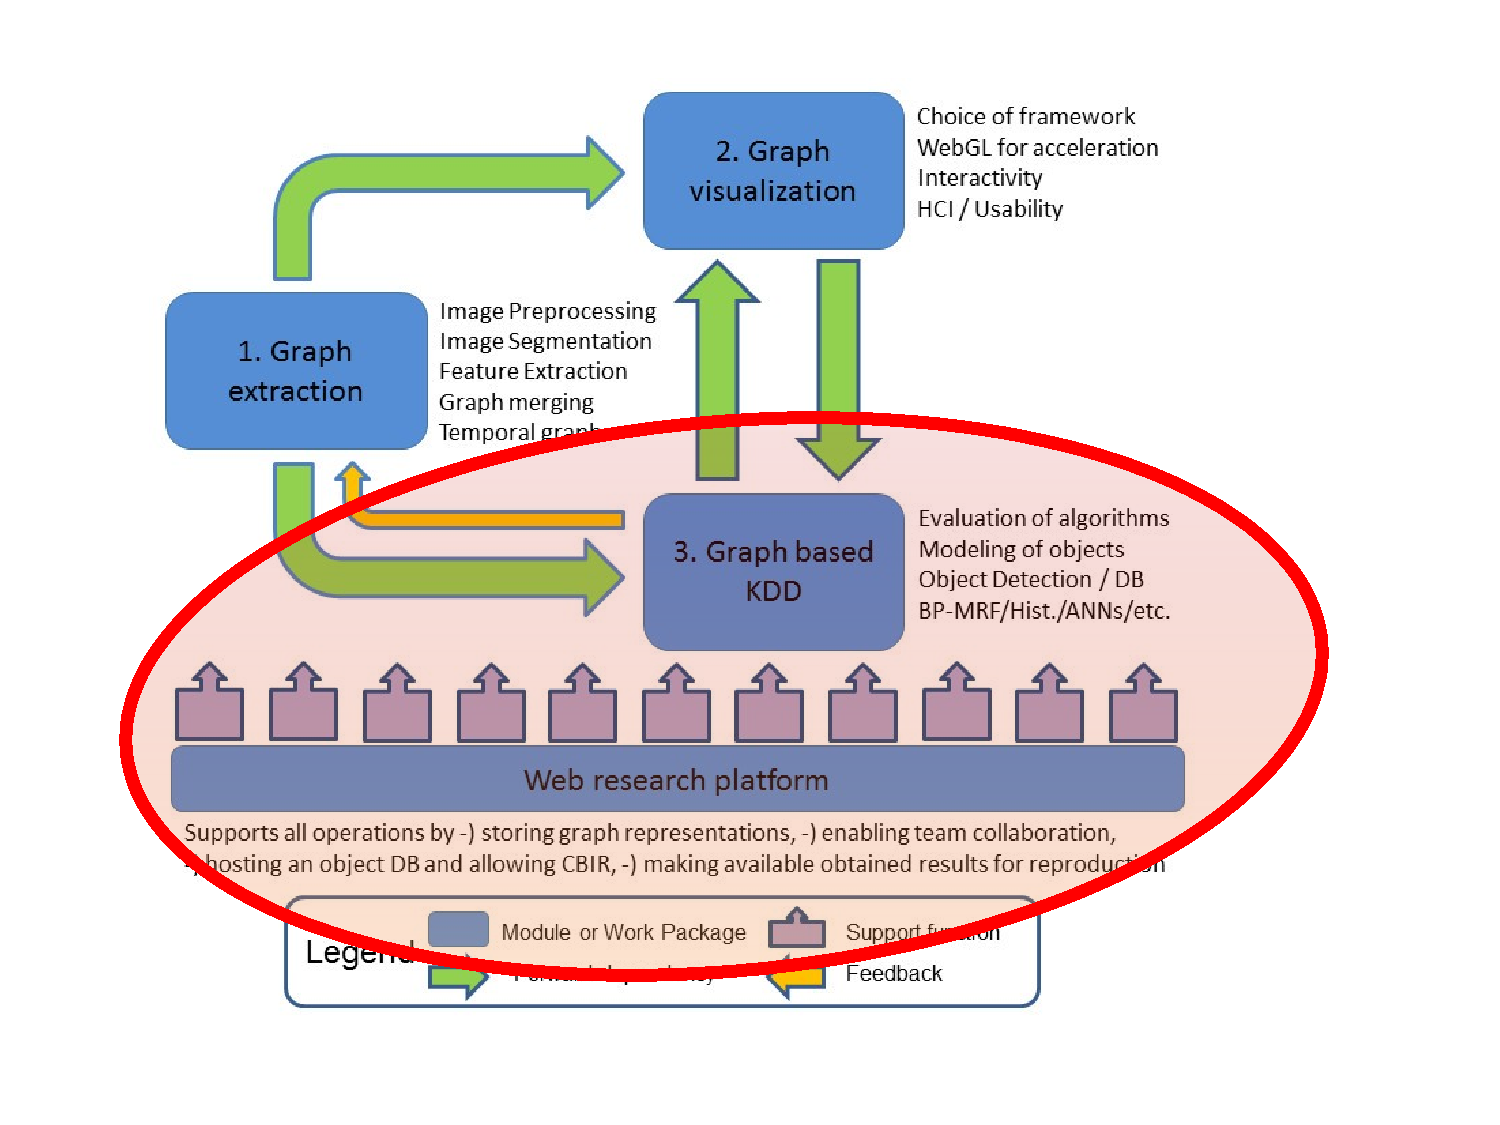
\includegraphics[width=1.1\textwidth]{figures/iKNOdis_OGMA_structure}
	\caption{Former project iKNOdis architecture overview}
\end{figure}


In the process of creating an FWF proposal out of iKnodis, the project was split into two separate projects in order to make them amenable to independent smaller funding efforts as well as different groups of developers working on their respective areas of interest yet maintaining their focus towards achieving the common goal. This resulted into iKNOdis now spanning graph extraction out of images as well as 3-dimensional visualization of the resulting graph structures via a Browser based method. 

The remaining modules of building a Web Based research platform as well as establishing graph mining algorithms able to tackle object recognition / image classification tasks usually covered by traditional image processing techniques, have been outsourced to project OGMA, the Open Graph Mining Architecture. Although it will be in the context of OGMA that this Master Thesis will play out, the resulting smart computational pipeline will also encompass the algorithms of iKNOdis. Indeed, a graph extraction algorithm already implemented during my Master's Project \cite{GraphExtractPaper} will be part of the test cases for the practical implementation found in later chapters of this work. 

\section{How this thesis is structured}
\label{section:thesis_structure}

The rest of this chapter is composed of a short description of how composite machine learning tasks are handled today followed by the question if a transition towards Web based technologies is feasible given the narrow implementation choices in that field. We will then explore in detail what benefits researchers as well as the whole research community could derive from conducting experiments on such a platform; therefore we have to outline potential properties and focal points of such a technology. Upon a short discussion of how the gathering of metadata about diverse ML/KDDM experiments as well as their results could open up new opportunities, we will envision a future recommender system for composing machine learning pipelines based on a heuristic approach. This chapter will close with a brief overview of the general properties of the smart computational pipeline (henceforth called ``SCP'') under development.

\par

Chapter 3, ``Related work'', will consider past and present approaches to recognizing objects in images as well as conduct image classification utilizing graph based approaches and will therefore show the validity of OGMA's objectives. Furthermore, contemporary efforts of building machine learning pipelines as well as the data and insights they are based on will be investigated. An overview of existing software solution will conclude chapter 2.

\par

In Chapter 4, ``SCP General Design'', we will lay the technical and scientific foundation for the design of a smart computational pipeline for OGMA. Building upon a high level overview of machine learning pipelines and their different stages in theory, we will be able to derive general requirements that any piece of software handling those processes will have to fulfill. Further, the question will arise as to how to represent algorithmic ``packages'' for the sake of this undertaking and how dependencies in the I/O of each pipelining stage should be resolved automatically. Following an analysis of how to use existing package manager algorithms to fulfill those requirements, the question of executing a valid processing pipeline within a browser environment considering modern users' expectations of fluidity and asynchronicity will be dealt with. At the end of this chapter, we will propose a data model for storing the experiment metadata for further analysis and find a description of the algorithms used for testing the pipeline later on.

\par

The next chapter 5, ``SCP Software Design'', will elaborate on the actual software implementation as well as the software development process followed in this project. First a set of requirements for modern Web based software will be compiled; based on this checklist an exploration of possible suitable technologies for both server and client will be conducted and their respective strenghts and weaknesses revealed. After a detailed comparison I will argue for the particular combination of choices I made and will subsequently describe the development process used to implement the pipeline. An illustration of how Webworkers were used to execute the pipeline as well as how results were visualized will finalize this chapter.

\par

The 6th chapter on ``Results and Discussion'' will wrap up the efforts undertaken in this project. I will first go into details about the project implementation and the difficulties and / or caveats that arose during my work. A detailed experimental setup will be described and the expected behavior of the SCP defined, while the ensuing section should verify those expectations and therefore validate the approach taken. A discussion of open and interesting challenges as well as  an outlook on future possibilities to enhance and expand on this work will top of this chapter.

\par 

Eventually the 7th and last chapter, ``Conclusion'', will give a short recap on the motivation, goals, and main issues of this project and thus bring the thesis to its completion.



\section{How Machine Learning / KDDM are approached today}
\label{sect:ml_kddm_today}

When taking the famous Machine Learning MOOC tought by Prof. Andrew Ng from Stanford University on Coursera in 2013, one story he was conveying during a section on optimizing Machine Learning Pipelines had especially caught my attention. As a specialist in high demand Prof. Ng is frequently consulting for Silicon Valley companies in matters of Machine Learning and Artificial Intelligence. On one of these occasions, the client company had been trying to optimize their ML pipeline for the better parts of 2 years without any significant improvements in their results. After looking at the different stages of their pipeline and conducting a so-called ceiling analysis, Prof. Ng concluded that two developers had spent 18 months on optimizing their background separation algorithm while the most significant potential for improvement really lay in a latter stage of the process. Based on this analysis the company was able to remedy the shortcomings in a relatively short amount of time.

\par

This incident shows how much effort is potentially squandered by trying to implement sophisticated processing pipelines within isolated teams in a non-standardized fashion: Proprietary approaches - both in technology as in methodology - hinder the exchange of information with other members of the research community, thus opening up vulnerabilities to making mistakes which could have easily been avoided by considering the experience of other professionals. The following properties of data analysis / ML projects seem to give rise to such vulnerabilities:

\begin{itemize}
	\item \textbf{Isolation.} Working on common machine learning problems in isolated teams without communication makes comparison of approaches as well as results unnecessarily hard. Dealing with errors at any stage of the pipeline takes more effort than necessary due to a lack of reference values, while achieving superb results has little to no effect on the potential of other experts.
	\item \textbf{Proprietary Software.} Countless professionals prefer developing data analysis pipelines in highly proprietary software environments like Matlab or Mathematica. This prevents an influx of solid, community-tested algorithms while preventing others from gaining knowledge acquired in such organizations (if they are unwilling to pay for the software).
	\item \textbf{Irreproducibility.} As unpublished code cannot be perfectly reverse engineered, experiments conducted in isolation can't be easily corroborated. This might be advantageous with respect to product development and patent procedures, but is usually detrimental to the efforts of researchers trying to get published and spreading their insights.
	\item \textbf{Lack of scalability.} Last but not least, heterogeneous and highly customized data processing pipelines might not lend themselves well to parallelization, which might prevent the use of such algorithms on quickly expanding datasets.
\end{itemize}


Papers to cite in this context: \\
\cite{LargeScaleMLPipelines}
\cite{MLPipelineMLlib}
\cite{DataAnalysisDSWorkflow}
\cite{StanfordNLP}
\cite{MLPipelines}
\cite{Make2013}
\cite{AnalLifecycle}
\cite{DataScienceTools2013}
\cite{AnalOneComponent2013}


\section{A Web based approach - why?}
\label{sect:web_transition}

\section{How a Web based approach could benefit users, researchers and society}
\label{sect:web_benefits}

\begin{itemize}
	\item \textbf{Ease of access.}
	\item \textbf{Effortless scalability.}
	\item \textbf{Built-in potential analysis.}
	\item \textbf{Server Side Meta Machine Learning.} As researchers start using our platform, their pipeline configurations, input descriptions, task specifiers (classification, text analysis etc.) as well as results will be stored on the server. Enough data provided, such a database might be amenable to the development of heuristics on the expected success of a particular algorithm invoked at a specific stage of the pipeline.
	\item \textbf{Heuristics-based recommendations.} Based on the last section, an optimal pipeline configuration might be computed provided only the input data (image, text, point cloud etc.) as well as the desired result. The Smart Computational Pipeline would then self assemble (given the user has no objections) and immediately commence the experiment.
\end{itemize}



\section{General applications}
\label{sect:ogma_focal_points}

\subsection{education}
\label{ssect:education}

\subsection{algorithm prototyping}
\label{ssect:algo_proto}

\subsection{research platform}
\label{ssect:research}



\chapter{Theoretical background / applications}
\label{ch:applications}


\section{Graph Theory}
\label{sect:graph_theory}


\section{Areas of application}
\label{sect:app_areas}

	\subsection{Social networks}
	\label{ssect:social_networks}
	
	Social networks are today's natural candidates for graph based algorithms, as they have been rising to power and fame over the previous decade and a half. Of course most social graphs in use today are far too big for any client or server side application to handle, and are therefore only interesting to programmers and architects of database clusters, high performance grid-computing developers and data-center engineers. Because of this, I am going to confine myself to the topic of local sphere recommenders, where I believe small graph computing to be able to have some real world influence. In order to get to this point, we will first need to take a look at the shape and size of typical recommendation processes (themselves forming subgraphs of larger networks), which in the following section will be termed 'cascades'.
	
	
	\subsubsection{Network recommendation analysis}
	\label{sssect:net_rec_anal}
	
	\citet{RecCascades} have examined recommendation networks crystallizing from purchases based upon previously received product recommendations. In order to do this, they employed an online shopping system observing the product categories of DVDs, Music, Books and Videos (VHS). Users of that system were modelled as nodes in a graph, with the graph initially being completely unconnected. In this system people who bought a product (and only actual purchasers) were able to recommend the bought product to as many people  as they wanted via email; this resulted in a \textit{temporary} recommendation edge added between the two (user) nodes. This edge was then handled according to the following two criteria:
	
	\begin{enumerate}
		\item Recommendations received after a product was already bought by the receiving person were immediately deleted.
		\item Recommendations received which did not result in the product being bought (during the observational period) were also deleted.
	\end{enumerate}
	
	This procedure resulted not in a graph comprising all of the users and products bought throughout the system, but only a collection of - fragmented - subgraphs representing the recommendation cascades. The main question of the study then was to the size distribution of those cascades w.r.t. their count, and if properties of the original social network (e.g. density, degree distribution) had any influence on that distribution. 
	
	A second point of interest concerned the isomorphism classes of cascades, meaning their shape and size similarity. Therefore, a similarity measure had to be established, as the graph isomorphism problem is NP-hard and therefore impractical to use on a real-world study. This is why exact isomorphism matching was only used on cascades up to a graph size of 9 nodes; above that a graph \textit{signature} was computed including singular values (via SVD) of the graph adjacency matrix up to a size of 500 nodes. Above that, the signature only consisted of the number of nodes and edges as well as a histogram of in- and out-edges per node (degree distribution). The relation between cascade amount and size can be seen in Figure~\ref{fig:cascade_size_count} on page \pageref{fig:cascade_size_count}.

	The results of this study after a two-year period can be summarized as follows:
	
	\begin{itemize}
		\item The largest cascade (which also form connected components) accounted for less than 2.5\% of all nodes.
		\item Cascades did not only come in the form of trees (snowball effect) but form arbitrary graphs with splits, collisions as well as cycles.
		\item Splits are more common than collisions, however (as one would expect).
		\item The frequency of a cascade type (as computed by graph isomorphism) is not a strict monotonic function of cascade size, which points to the recommendation propagation process to be influenced by more subtle factors of the underlying social graph than just the network structure alone.
		\item Most cascades observed exhibited fewer than 9 nodes (with the exception of DVD recommendation cascades) and were of very small degree (just a little over 1 according to the visual representation found in the paper
	\end{itemize}
	
	\begin{figure}[ht]
		\begin{center}
			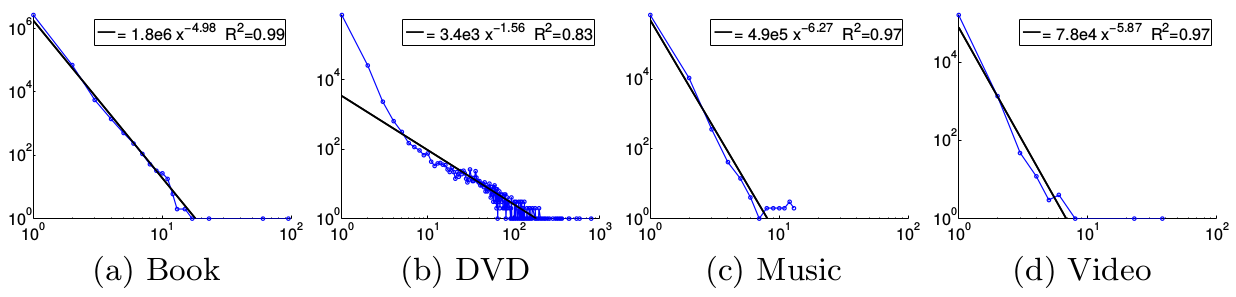
\includegraphics[width=1\textwidth]{figures/rec_cascades_size_count}
			\caption{Size distribution of recommendation cascades for four product categories}
			\small
			This diagram was taken from \citep{RecCascades}, page 7.
			\label{fig:cascade_size_count}
		\end{center}
	\end{figure}
	
	The above analysis holds several insights which in combination lead to a remarkable conclusion:
	
	\begin{enumerate}
		\item The cascades presented in the paper represent only 'successful' recommendations, i.e. the ones which receivers perceived as valuable enough to actually buy the product.
		\item The goal of any recommender algorithm (regardless on which item space it operates) is to produce exactly such valuable recommendations.
		\item Because most cascade sub-graphs were of very small size and degree, 'successful' recommendations can be assumed to originate from places in the direct neighborhood of a node.
	\end{enumerate}
	
	
	\subsubsection{The local sphere}
	\label{sssect:the_local_sphere}
	
	The concept of a local sphere and computations applied to it comes from the author's (possibly incorrect, but natural) insight that the relevance of recommendations behaves as a function of node vicinity:
	
	\begin{itemize}
		\item Lets call the whole social graph and all interactions in it the 'global sphere'.
		\item Recommendations to users are then computed over the global sphere, which takes an amount of resources exponential to the size of the underlying graph.
		\item Let's further assume that 95\% of all relevant (accepted) recommendations in a social network like facebook are those that are derived from the immediate local neighborhood of a node (less than 2 degrees, see section above..)
		\item This assumption is corroborated by the fact that two degrees are also what Facebook allows programmers (as of 2013) to query via their graph API from any authenticated user, apparently in an effort to prevent automatic traversal / exploration of their most valuable business asset.
		\item Let's call this immediate local neighborhood the 'local sphere'
	\end{itemize}
		
	Now let's also consider how modern publish/subscribe based frameworks (like Sails, Meteor, Hapi or Derby, only to mention some JavaScript libraries) handle data communication between server and client:
	
	\begin{itemize}
		\item The server offers some subscriptions on it's data, usually limiting access to items based on identity, authorization or user role provided by the client.
		\item The client defines some subscriptions on server-side data collections (tables), representing the client's wish for information regardless of it's status or authority.
		\item Publication as well as subscription can be seen as a mathematical subset of all the data in the database.
		\item An algorithm inside the respective framework resolves those (potentially conflicting) interests by computing the intersection set of the data provided / requested.
		\item The intersection data set is then pushed to the client (in our case the browser) as soon as it becomes available or is updated, which makes this model ideal for real-time interaction and communication between clients.
		\item The sum total of all the data pushed to the client is equivalent to the 'local sphere' we described earlier - HOWEVER - their inherent graph structure is lost during the transmission, so that the client can only see them as isolated fragments without context.
	\end{itemize}
	
	The combination of those two ideas now enables us to envision the following scenario:
	
	\begin{itemize}
		\item Instead of interpreting all data items in the local sphere as isolated entities, we retain their graph structure enabling the client to gain hitherto unachieved knowledge and insights into its already available data.
		\item We therefore need a graph library in the browser, not only to represent the local sphere graph, but also to analyze it in order to take intelligent actions that were previously reserved for the server-side (data center) infrastructure.
		\item No complex graph partitioning algorithm on the server is necessary, as we can use the natural set contraints inherent in any web application:
		\begin{itemize}
			\item e.g. in a social network, the client will have access to all its immediate friends, social activities and interest groups
			\item in a project management tool, the client naturally has access to the data of all team members, to-do lists, milestones, resources etc.
		\end{itemize}
		If our 95\%-relevance assumption mentioned earlier holds, we can achieve great scaling efficiency by introducing the local sphere concept:
		\begin{itemize}
			\item the client can immediately perform computations like recommendations on the subgraph of the local sphere.
			\item only recommendations accepted will have to be stored on the server (that is, cause additional network traffic).
			\item the client is easily able to recompute the relatively small local graphs in real-time, offering responsiveness far beyond today's best (server-side) infrastructures.
			\item as modern web frameworks transport all of the required data into the client store anyways, we do not add extra complexity to our servers and databases.
		\end{itemize}
		\item On the other hand, questions of data security / privacy will have to be dealt with, as we are talking about preemptively filling the client memory with possibly otherwise unnecessary or superfluous data.
	\end{itemize}
	
	
	\begin{figure}[ht]
		\label{fig_local_sphere}
		\begin{center}
			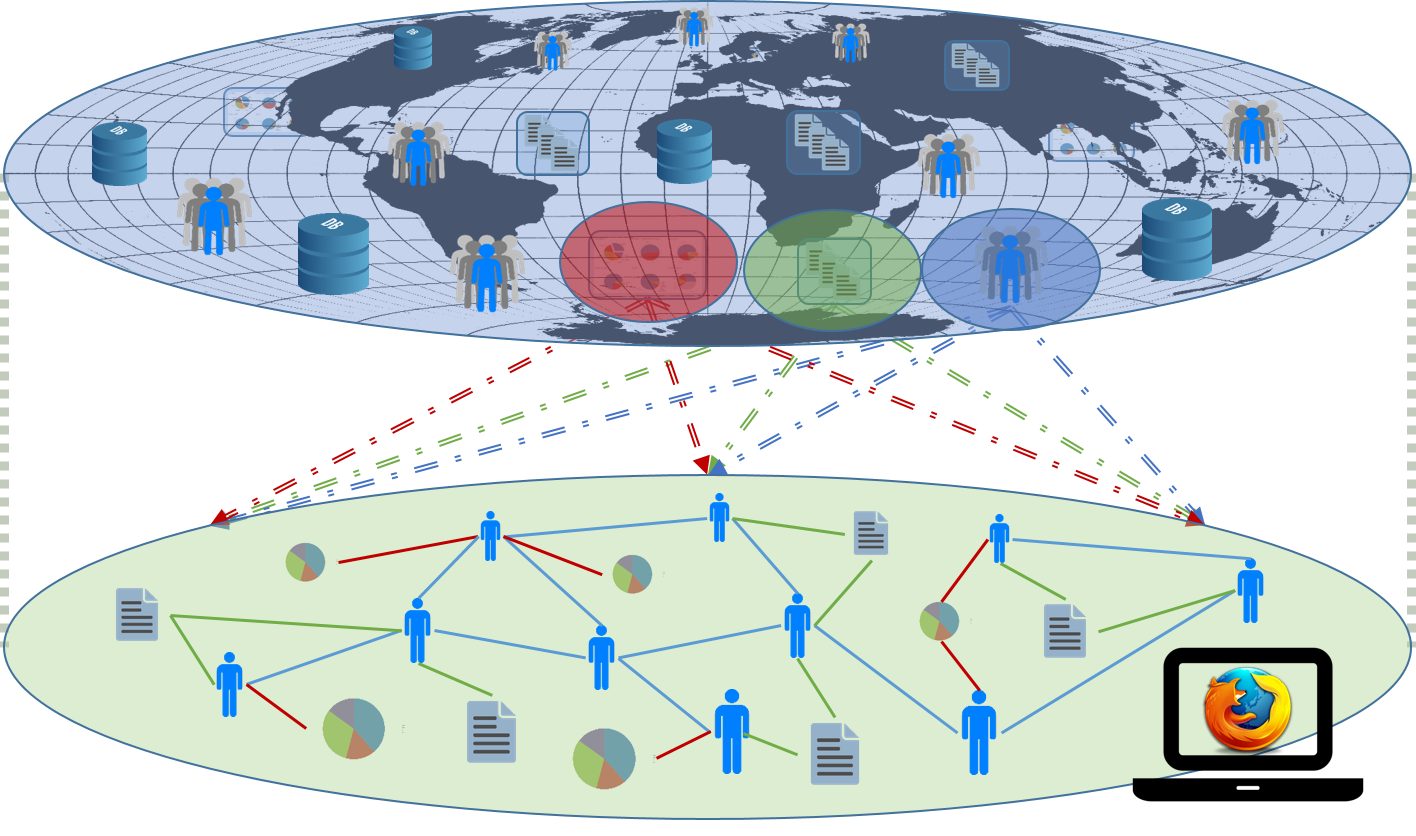
\includegraphics[width=1\textwidth]{figures/local_sphere}
			\caption{Local sphere projected from global sphere}
		\end{center}
		\small
		Only a very small portion of the global graph is actually visible from any connected client. The sum of all viewable items however, if properly conveyed to the client (i.e. with their connection information preserved), could form a subgraph of the whole network called the 'local sphere', which would allow the browser to utilize the underlying graph structure to extract hidden knowledge and perform graph computations on its own.
	\end{figure}
	
	
	Needless to say, GraphiniusJS would be an ideal candidate to explore this concept further and could, if used appropriately on carefully modeled local spheres, enable start-ups to compete with much larger companies employing complex and very expensive machine learning infrastructures.
	
	
	% \subsection{Communication networks}
	% \label{ssect:app_communication_networks}
	
	% \subsection{Transportation networks (Logistics)}
	% \label{ssect:app_transportation_networks}
	
	
	\subsection{Graph based image processing}
	\label{ssect:app_graph_img_proc}
	
	\begin{figure}[ht]
		\label{fig_graph_based_img_classification}
		\begin{center}
			
\includegraphics[width=1\textwidth]{figures/graph_img_class}
			\caption{Graph based image classification example}
		\end{center}
		\small
		1) a laser scan image of a nevus is oversegmented and 2) a graph extracted by interpreting region centroids as nodes and region adjacency as edges. 3) A belief propagation algorithm is applied to the resulting graph yielding 2) a converged state representing the nevus classification as benign or malignant.
	\end{figure}
	
	\subsection{Graph based NLP}
	\label{ssect:app_graph_nlp}
	
	\subsection{Biomedical applications (protein networks etc.)}
	\label{ssect:app_biomed}
	
	\subsection{Anonymization}
	\label{ssect:app_snonymization}
	
	\begin{figure}[ht]
		\label{fig_graph_based_img_classification}
		\begin{center}
			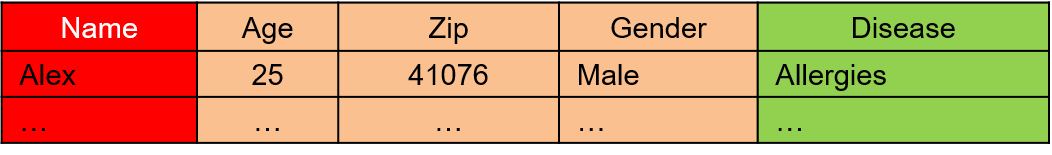
\includegraphics[width=0.9\textwidth]{figures/anonym/3typesofdata}
			\caption{The three types of data considered in (k-)anonymization}
		\end{center}
	\end{figure}
	
	
	\begin{figure}[H]
		\centering
		\begin{minipage}[b]{0.5\textwidth}
			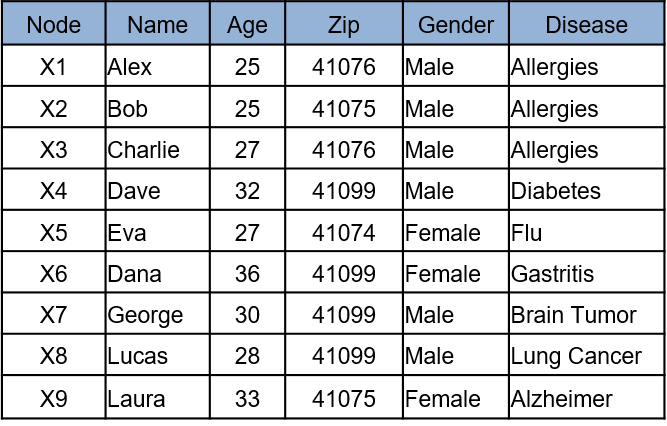
\includegraphics[width=\textwidth]{figures/anonym/k_anon_input}
		\end{minipage}
		\hfill
		\begin{minipage}[b]{0.418\textwidth}
			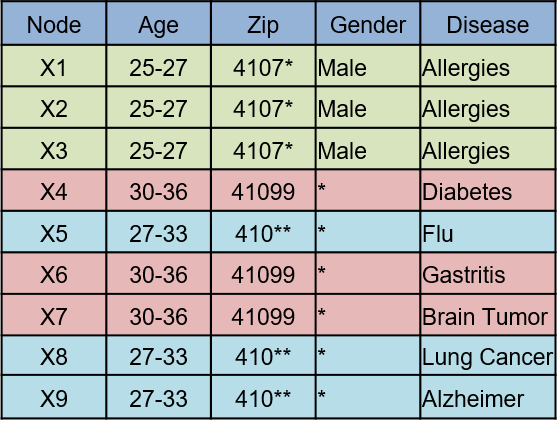
\includegraphics[width=\textwidth]{figures/anonym/k_anon_output}
		\end{minipage}
		\caption{Tabular anonymization: input table and anonymization result}
	\end{figure}	
	
	
	\subsection{Fraud detection}
	\label{ssect:fraud_detection}

	Polo chau's BP in MRF for spam classification work...

\section{Application specific requirements}
\label{section:app_requirements}

	\subsection{Data Structures}
	\label{ssect:data_gathering}
	
	\subsection{Data Cleaning}
	\label{ssect:data_cleaning}
	
	\subsection{Preprocessing}
	\label{ssect:preprocessing}
	
	Graph generation (ER model...)
	
	\subsection{Feature Selection}
	\label{ssect:feature_selection}
	
	\subsection{Data Mining}
	\label{ssect:data_mining}
	
	\subsection{Postprocessing}
	\label{ssect:postprocessing}
	
	\subsection{Visualization}
	\label{ssect:visualization}
	
	\subsection{Interaction / user feedback (iML)}
	\label{ssect:interaction}
	

\chapter{GRAPHINIUS as a platform}
\label{ch:graphinius_platform}


\section{General Properties}
\label{sect:general_properties}
	
	\subsection{Automatic real-time visualization (switchable)}
	\label{ssect:realtime_vis}
	
	\subsection{Online documentation}
	\label{ssect:online_doc}
	
	\subsection{Example graph datastructures}
	\label{ssect:pre_settings}
	
	\subsection{User profiles}
	\label{ssect:user_profiles}
	
	\subsection{Save and fork experiments}
	\label{ssect:save_fork}
	
	\subsection{Distributable via URL (like e.g. Codepen)}
	\label{ssect:distribute_url}
	
	\subsection{Can write own algorithm and use on given graphs}
	\label{ssect:define_algos}



\section{Graph Properties}
\label{sect:graph_properties}

	\subsection{Mixed mode graph}
	\label{ssect:mixedmode}
	A mixed mode graph - at least in Gephi vocabulary - is a graph that may contain directed as well as undirected edges at the same time. While many algorithms are defined on just undirected (e.g. Minimum spanning tree) or directed (e.g. percolation) edges exclusively, for many real world applications it is required to consider a combination of both - imagine traffic simulations with one-way streets or social networks in which people can be friends (undirected) and / or follow each other (directed). As Graphinius should be able to cover such applications, its core needs to be designed as a mixed-mode graph; the problem with this is that many algorithms have no standard implementation for a mix of both edge types, and so here and there it was necessary to come up with a logical and pragmatic solution, even if it could not be verified by any textbook.
	
	\subsection{Node and edge types (filters)}
	\label{ssect:node_types}	
	A mixed-mode graph alone however, is not enough for more complex scenarios, even in every day's situations. Assuming a social network again, we would first think of humans as participating entities. Depending on the particular use case of the network however, other nodes might be resources such as books (author network), movies (Netflix), or any type of commodity (online shopping). Moreover, edges in such a network cannot only differ in mode of direction, but might represent a specific type as well (following someone vs. movie recommendation). From this emerges the need for graph filtering - or graph views - which expose only a specified subgraph to an executing algorithm, suitable to the particular situation. To stay with our example, if we need to find all users within three hops of friendship connections, we do not want to traverse all the edges representing recommendations (or messages, as there might be orders of magnitudes more of those present). In this case, we would execute a Breath-first-search against a view of the graph, which would present the BFS's logic with only the connections it is required to 'see'.
	
	% TODO INSERT GRAPHIC
	
	\subsection{Object oriented}
	\label{ssect:oo}
	One design decision in writing any new (graph) library - as far as the author can judge from his personal research - lies in speed and memory vs usability. This concerns not so much the handling of nodes and edges themselves (many libraries have very good wrapper functions for dealing with basic primitives), but requirements like additional payload - e.g. the k-gram vector of a node representing a text document - or node \& edge types themselves. In order to speed up execution of graph algorithms, advanced libraries use specialized data types like sparse matrices or fixed-length arrays; this on the other hand forces a programmer to hold additional data structures at hand for whenever more complex computations are needed. A good example for this would be computing the 'distance' of two nodes when defined not as the length of the shortest path between them, but as the cosine distance between their feature vectors. \\
	
	Taking into account the special language properties of Javascript, with its great emphasis on first-order functions and closures which makes for a natural callback-driven algorithmic approach (see fig. [insert figure]), the author believes that an object oriented approach is the suitable one for Graphinius, which is backed by 3 different properties of the language:
	
	\begin{itemize}
		\item Despite not being 'traditionally' object oriented like Java or C++ for its absence of constructs like classes etc., Javascript is firmly OO - in fact, everything except primitives is always an object, including and especially functions.
		\item Accessing objects instead of flat memory should not incur too much runtime overhead anymore, since modern JSVMs have abandoned the flat model in favor of an object memory model themselves.
		\item As Graphinius is intended to be part of a learning, teaching and research platform, and not designed to handle large graphs of millions of nodes and upwards, the OO approach seems a natural fit since it allows implementing algorithms in a very intuitive way [comparison].
	\end{itemize}



\section{Online Editor}
\label{sect:online_editor}

	\subsection{Build \& mutate}
	\label{ssect: build_edit}
	
	\subsection{fork \& extend}
	\label{ssect: fork_extend}
	
	\subsection{publish via simple URL}
	\label{ssect: publish_url}



\section{Real world suitability}
\label{sect:realworld_suitability}

	\subsection{Collaborative platform (research teams)}
	\label{ssect:collaborative_platform}

	\subsection{Reproducibility / Corroboration of results}
	\label{ssect:reproducibility}
		
	\subsection{Prototyping}
	\label{ssect: prototyping}



\section{Algorithm Marketplace}
\label{sect:algo_marketplace}

\subsection{personal algorithms}
\label{ssect:algo_personal}

\subsection{community algorithm database}
\label{ssect:community_algo_db}


	

% \chapter{Related Work - Survey of graph libraries}
\label{ch:related_work}



\section{C++}
\label{sect:cpp}

	\subsection{Boost Graph Library (BGL)}
	\label{ssect:bgl}
	
	\subsection{Lemon (C++)}
	\label{ssect:lemon}
	
	\subsection{igraph (c, python, R)}
	\label{ssect:igraph}
	
	\subsection{GraphTool}
	\label{ssect:graphtool}



\section{Java}
\label{sect:java}

	\subsection{GraphStream}
	\label{ssect:graphStream}
	
	\subsection{JUNG}
	\label{ssect:jung}
	
	\subsection{JGraphT}
	\label{ssect:jgrapht}
	
	\subsection{Grph}
	\label{ssect:grph}



\section{Python}
\label{sect:python}

	\subsection{Networkx}
	\label{ssect:networkx}



\section{Ruby}
\label{sect:ruby}

	\subsection{graphy}
	\label{ssect:graphyphStream}
	
	\subsection{RGL}
	\label{ssect:rgl}



\section{Other (Matlab, R, whatever)}
\label{sect:other}

	\subsection{The R graph package (discontinued, just mention)}
	\label{ssect:rgraph}
	
	\subsection{Matlab BGL}
	\label{ssect:matlab_bgl}
	
	\subsection{Graphs.jl (Julia)}
	\label{ssect:graphjl}
	
	\subsection{scala-graph}
	\label{ssect:scala_graph}
	
	\subsection{Cassovary (JVM, written in Scala)}
	\label{ssect:cassovary}
	
	\subsection{loom (Clojure)}
	\label{ssect:loom}
	


\section{Graph visualization tools}
\label{sect:graph_visualization}

	\subsection{Gephi}
	\label{ssect:gephi}
	
	\subsection{GraphViz}
	\label{ssect:graphviz}
	
	\subsection{Infovis}
	\label{ssect:infovis}
	
	\subsection{D3.js, plotly(js), Sigma, Cytoscape, vis.js (JS), Vivagraph}
	\label{ssect:js_based_vis}



\section{Why YAGL (Yet another graph library) in JS?}
\label{sect:why_yagl}

	\subsection{runs in the browser as well as on the server via node.js}
	\label{ssect:browser}
	
	\subsection{browser makes integration with visualization libraries a breeze}
	\label{ssect:vis_integrate}
	
	\subsection{no installation necessary}
	\label{ssect:no_inst}
	
	\subsection{could run via dnd ui interface (no programming needed)}
	\label{ssect:no_prog}
	
	\subsection{extendable via server-side snippets of source code (algo database)}
	\label{ssect:extendable}



% \chapter{Architecture of GRAPHINIUS}
\label{ch:graphinius_architecture}

\begin{figure}[ht]
	% \centering
	\hspace*{-0.5cm}
	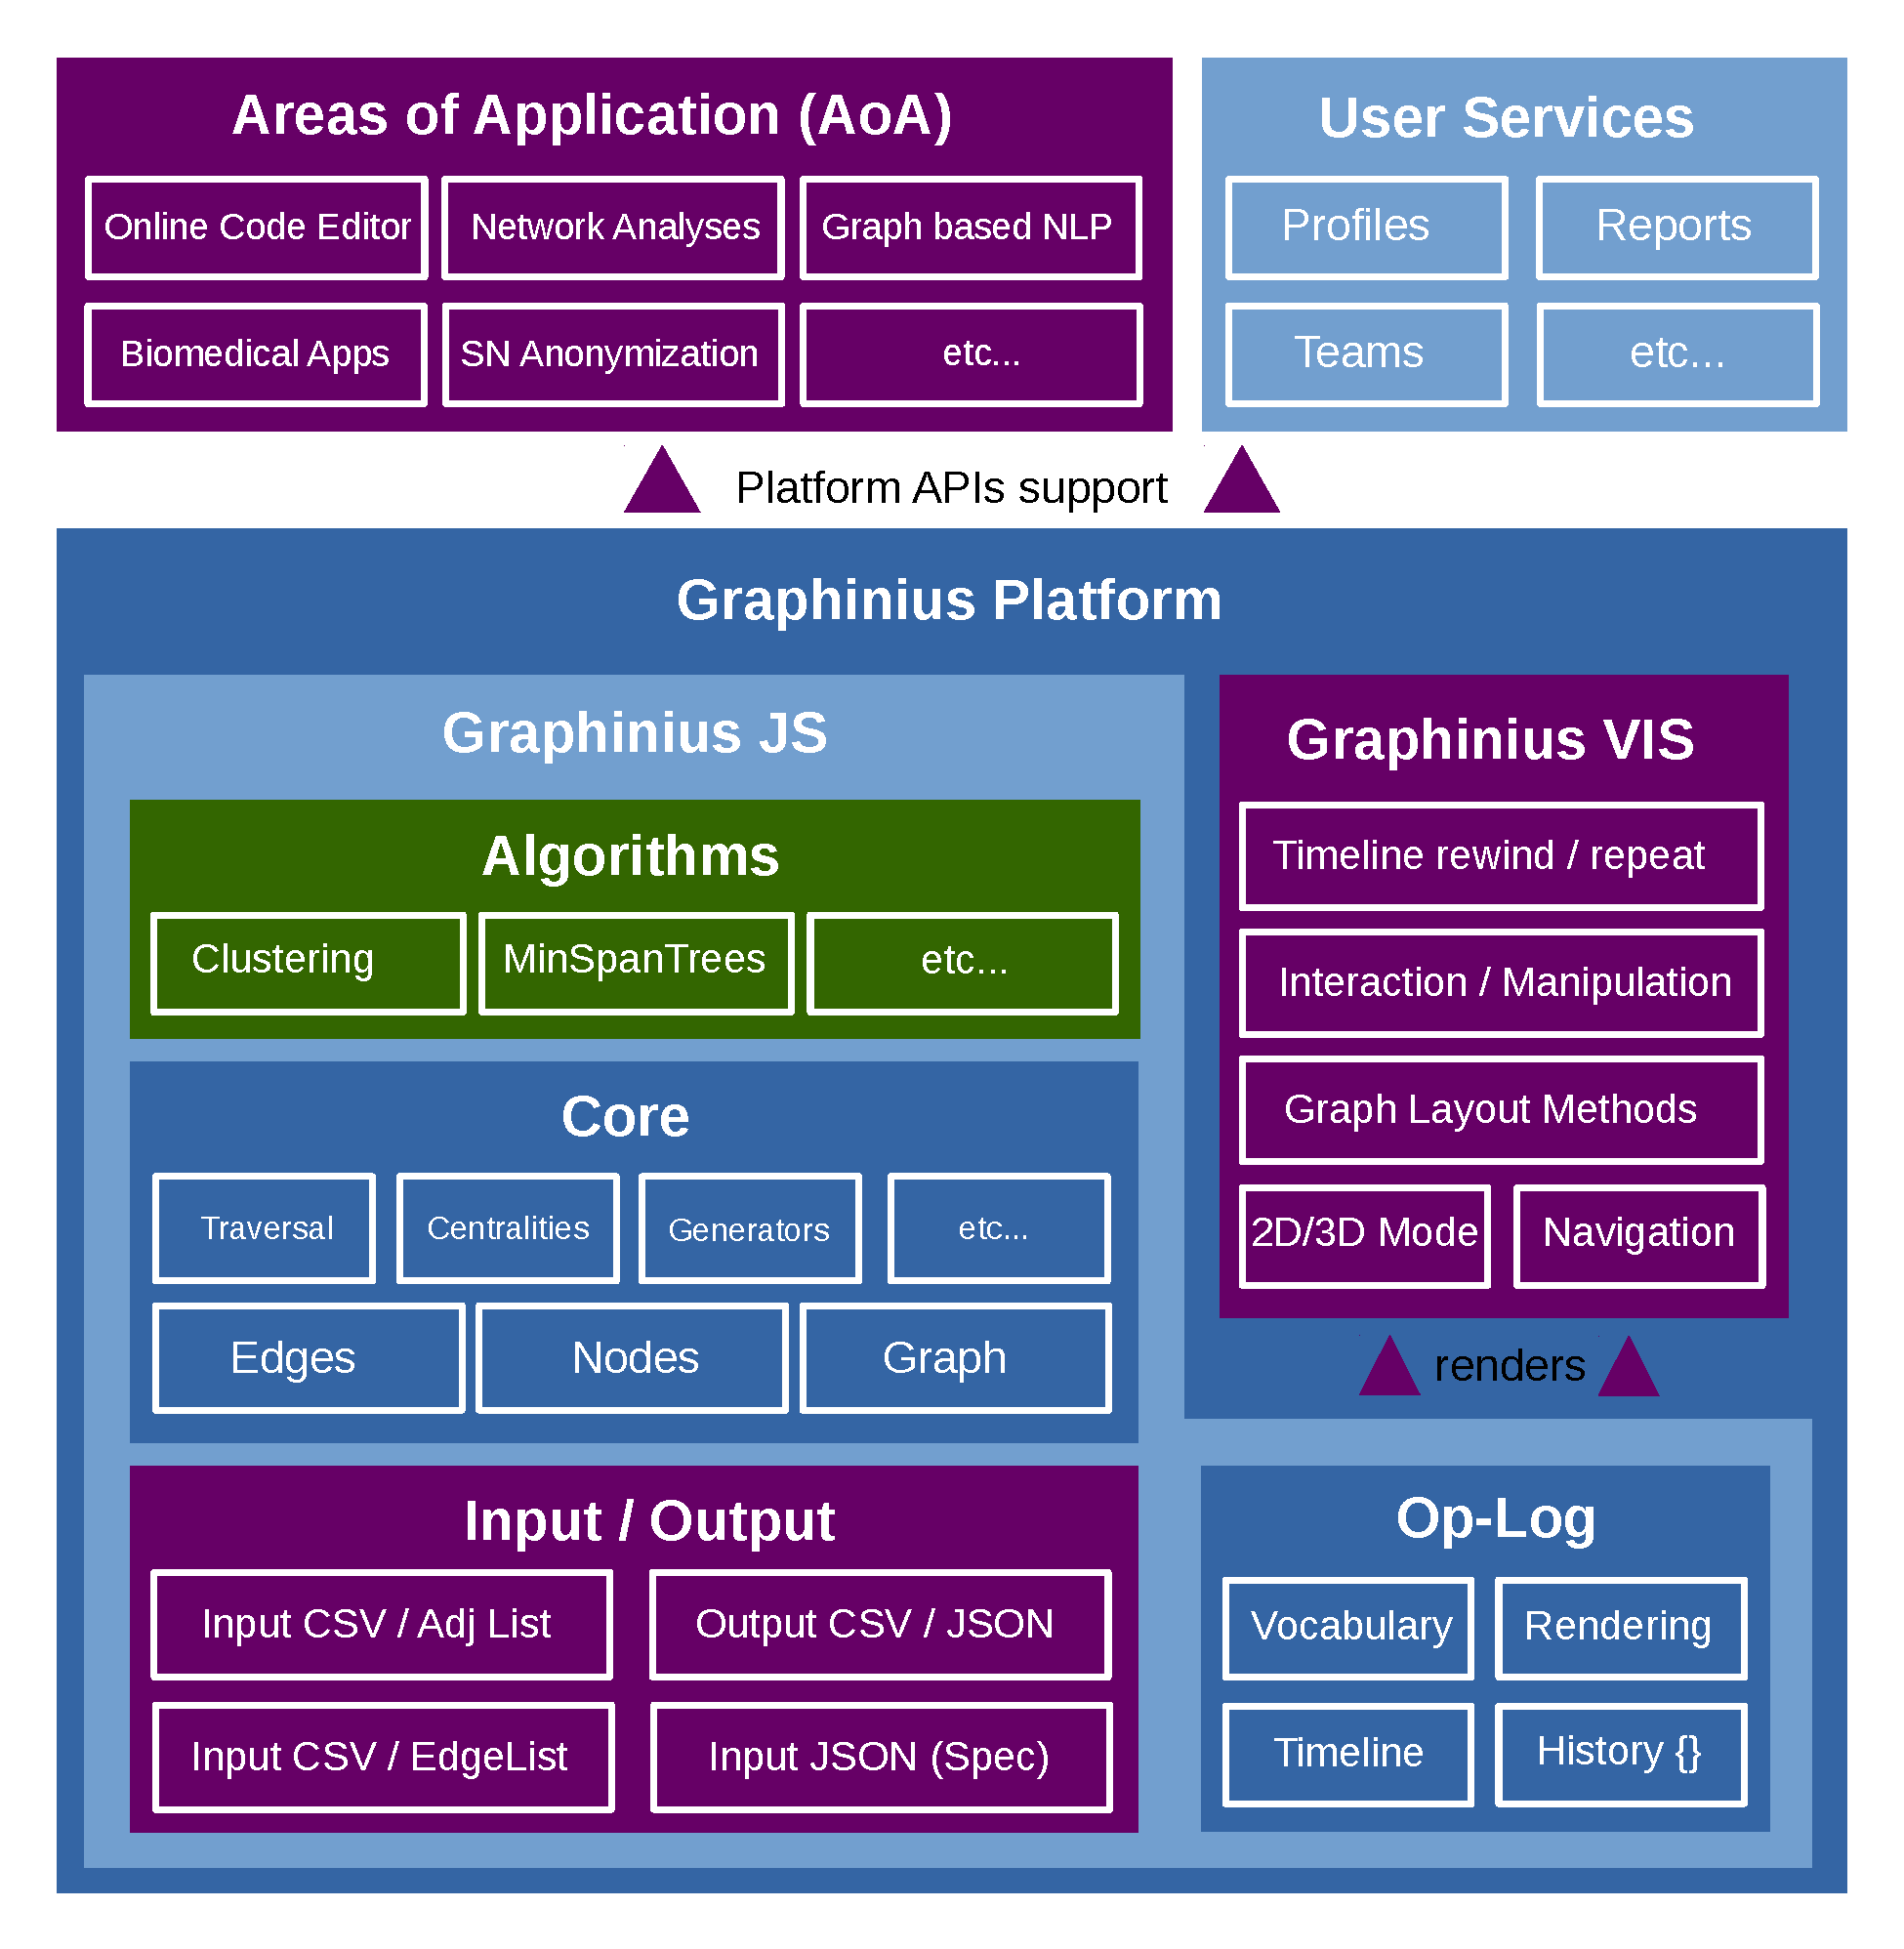
\includegraphics[width=1.1\textwidth]{figures/Graphinius_Architecture_pdf}
	\caption{Graphinius platform architecture overview}
	\label{fig_graphinius_architecture}
\end{figure}



\section{Graphinius Base}
\label{sect:graphinius_base}

As the name suggests, the Base offers all the functionality necessary to develop graph-based applications on top of it, including basic graph-computations and algorithms as well as visualization. It is therefore logically composed of those two modules, Graphinius JS and Graphinius VIS as well as a mechanism of communication between those two.
	

\section{Graphinius JS}
\label{sect:graphinius_js}

	\subsection{Graph input readers}
	\label{ssect:input_output}
	
		\subsubsection{CSV}
		\label{sssection: io_csv}
		
		
		\begin{figure}[ht]
			\begin{lstlisting}
				A, B, u, C, u, A, d, B, d, D, d
				B, A, u
				C, A, u, A, d
				D, A, d
			\end{lstlisting}
			\caption{Adjacency list including edge direction}
			\label{fig:adj_list_direction}
		\end{figure}
		
		CSV Edge Lists use the simple format of [StartNode, EndNode [,directed]].		
			
		
		\subsubsection{JSON}
		\label{sssection: io_json}
		
		\begin{figure}[ht]
			\centering
 			\hspace*{-1.5cm}
			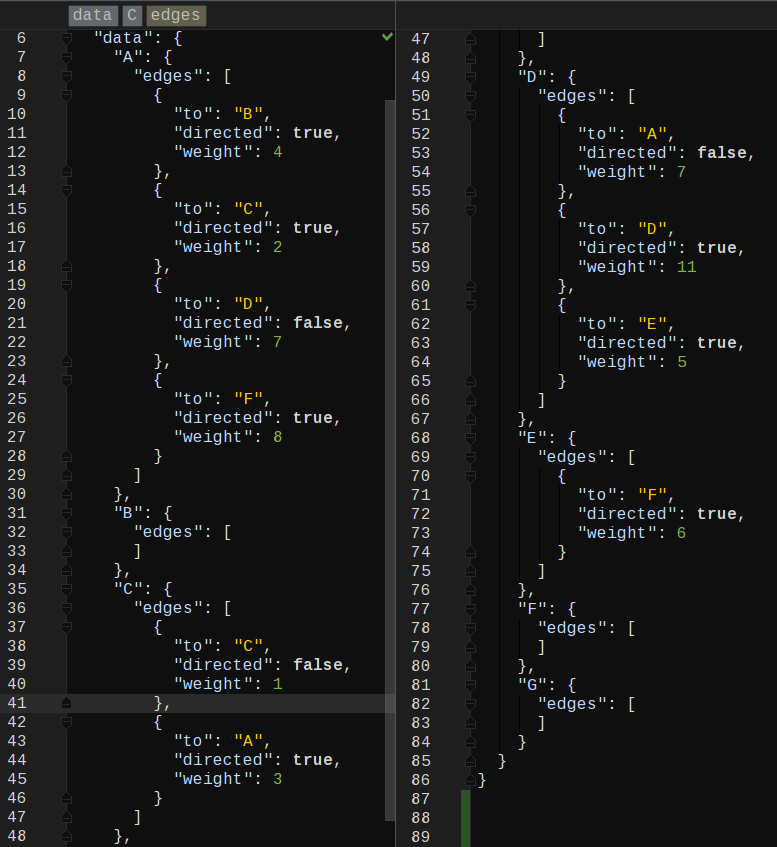
\includegraphics[width=1.2\textwidth]{figures/search_graph_json}
			\caption{Sample graph in the Graphinius JSON format}
			\label{fig:json_input_graph}
			\small Apart from the 'to' node, direction and weight, any node can exhibit an arbitrarily large feature vector containing any type of information (like patient data, word vectors, etc.). Another special sub-object which the input reader is looking for is the 'coords' object, which specifies the coordinates used in the constant layout renderer of the GraphiniusVIS library.
		\end{figure}
		
	
	\subsection{Graph Core}
	\label{ssect:graph_core}
	
		\subsubsection{Edges}
		\label{sssection: core_edges}
		
		\subsubsection{Nodes}
		\label{sssection: core_nodes}
		
		\subsubsection{Graph}
		\label{sssection: core_graph}
		
		\subsubsection{Traversal}
		\label{sssection: core_traveral}
		
		BFS / DFS implementations... [figure: callback-based DFS]
		
		\subsubsection{Degrees}
		\label{sssection: core_degrees}
		
		\subsubsection{Centralities}
		\label{sssection: core_centralities}
		
		\subsubsection{Generators}
		\label{sssection: core_}
		
	
	\subsection{Algorithms}
	\label{ssect:algorithms}
	
		\subsubsection{Clustering}
		\label{sssection: algo_clustering}
		
		\subsubsection{MinSpanTrees}
		\label{sssection: algo_minspan}
		
		\subsubsection{Shortest Paths}
		\label{sssection: algo_shorest_paths}


\section{The Op-Log}
\label{sect:op_log}

	\subsection{Timeline}
	\label{ssect:timeline}
	
	\subsection{History Object}
	\label{ssect:history_object}

	\subsection{Vocabulary}
	\label{ssect:vocabulary}	

	\subsection{Rendering Mechanism}
	\label{ssect:rendering}


\section{Graphinius VIS}
\label{sect:graphinius_vis}

	\subsection{2D/3D Mode}
	\label{ssect:vis_2d3d}
	
	\subsection{Navigation}
	\label{ssect:vis_navigation}
	
	\subsection{Graph Layouts}
	\label{ssect:vis_layouts}	
	
	\subsection{Interaction / Manipulation}
	\label{ssect:vis_interact_manipulate}
	
	\subsection{Timeline rewind / repeat}
	\label{ssect:vis_timeline}


\begin{landscape}
\begin{figure}[ht]
	\label{fig_history_workflow}
	\centering
	\vspace{-2.0cm}
%	\hspace*{0cm}
	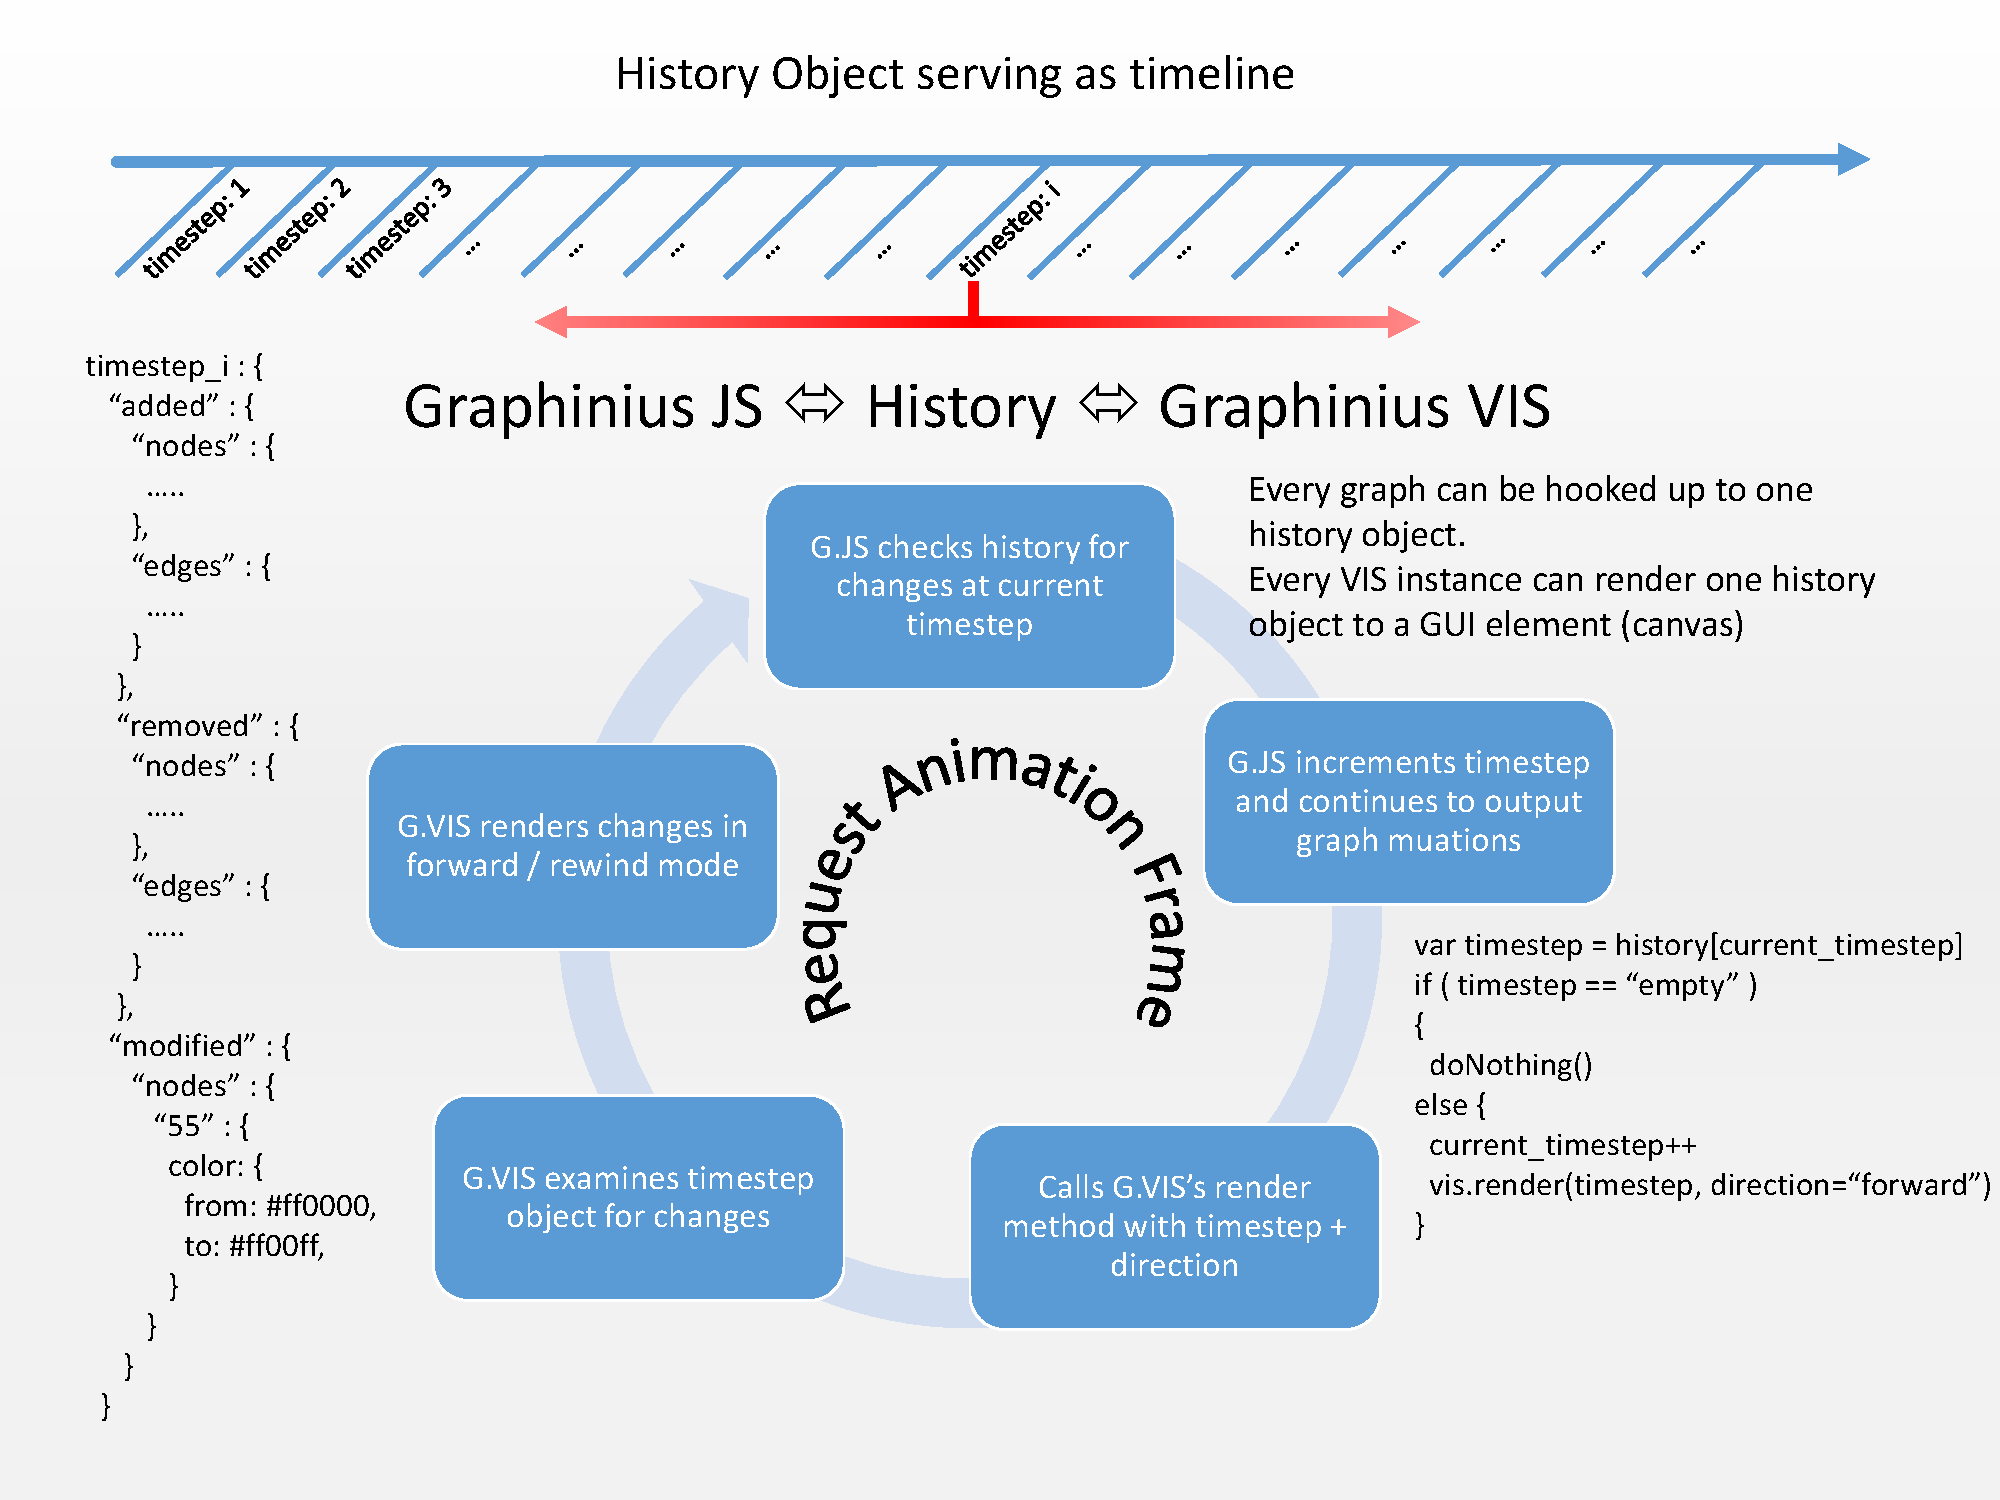
\includegraphics[width=1.6\textwidth]{figures/History_Workflow_pdf}
	\caption{Graphinius JS <-> VIS communication via Op-Log}
\end{figure}
\end{landscape}


\section{Areas of Applications (AoA)}
\label{sect:areas_of_applications}

	\subsection{Online Editor}
	\label{ssect:aoa_editor}
	
	\subsection{Biomedical Applications}
	\label{ssect:aoa_bioapps}
	
	\subsection{SN Anonymization}
	\label{ssect:aoa_anonym}


\section{Platform Services}
\label{sect:platform_services}

	\subsection{Personal Profile}
	\label{ssect:service_profile}
	
	\subsection{Teams}
	\label{ssect:service_teams}
	
	\subsection{Output / Reports}
	\label{ssect:service_output}

\chapter{Software Requirements \& Survey}
\label{ch:software_requirements}

In order to assess which technologies to use for a new project, one first has to take into account the kind of software product to build, the sector of the economy it will be used in as well as the specifics and constraints of the environment it's going to operate and interconnect in. Let us first take a closer look at those points:

\begin{itemize}
	\item \textbf{The kind of product} to construct will often determine some core technologies: Building a messenger app requires real-time behavior some statistical product suite would never make use of. Likewise, an autonomous control system of a space probe will also depend on time-critical components, but in a different way than a messenger app, relying strongly on a constant rate of throughput, whereas a message flow will not be critically disturbed by a lag or latency disruption every now and then.
	\item \textbf{The industry sector} largely determines requirements in the form of compliance or industry certification. For instance, whereas the security concerns in a normal end-user centered application might be dealt with with relatively moderate levels of effort, applications employed in the financial or even medical sectors will in all probability have to satisfy additional security demands such as audit trail systems or compliance to specific data formats and standards.
	\item \textbf{The technical environment} a system is operated in will influence its shape and behavior as well. A relatively disconnected and isolated system like a statistical module (which e.g. outputs some results on a nightly basis) will be modeled differently than a web-based, cloud-oriented service incorporating many interfaces and API calls to dependent background or partner services.
\end{itemize}

In the following sections, we are not considering the entire SW development workflow from an economic / managerial point of view, but just the technological aspects of it. Let us first realize the differences between software development today and the way it was usually conducted as short as only 2 decades ago.

The traditional software development process as followed throughout the first decades of the existence of our field has been relatively simple: upon setting a goal for functionality or any other measurable entity (code module, UI section), a continuous iterative process of writing some lines of code, re-compiling, testing (automated or manual) and bug fixing was all, or most, that was necessary to arrive at some usable product. Modern applications, however, especially web-based ones (and that includes all kinds of mobile apps that have seen their rise over last decade) operate on many different moving parts:

\begin{itemize}
	\item Some server-side backend which coordinates incoming requests and provides consistency across business logic and database layers. This is probably the part with the greatest similarity to traditional, client-only or centralized software (development). I would also include old-fashioned web 'applications' (and certainly websites) in this environment, as a browser-based GUI alone without much processing or business logic going on, does not really fall into the category of a distributed application.
	\item A client part in the form of a modern in-browser based app (like GMail, Google Docs or Office365) or any mobile app executing on a contemporary mobile device.
	\item Some background-services, mostly in separated modules distributed over one or many servers worldwide, including interfaces to dependent services, isolated REST services (like a search portal for medical professionals inside a larger healthcare application) or microservices: sub-components of the business logic implemented directly on a database level, as implemented in the Foxx application micro-framework inside the multi-model database ArangoDB \citep{Foxx2014}.
	\item Where needed, a visualization module will have to be provided which resides on the client side but is logically separated from the 'normal' business and communication logic of that module. In browsers, this can either be written in normal DOM code, SVG, Canvas, or WebGL (we don't want to mention earlier technologies that are fortunately falling from grace rapidly...).
\end{itemize}

In addition to this generic complexity, we have to deal with a different workflow cycle even on the level of individual developers: Whereas 15 years ago somebody could set up some HTML files, include some JavaScript files, iteratively add new snippets of code and check the results by reloading the browser, even this small part of the development cycle has changed dramatically over the past 10 years - new Meta-languages like Typescript or Coffeescript on the language side, HTML-meta-markups like HAML, CSS preprocessors like Sass/Scss/Less as well as the integration of modern testing libraries makes a simple browser reload a technique of the past.

Those new methods provide great opportunities (but also challenges) even for the single programmer, which require a whole execution and deployment infrastructure, as depicted in Figure~\ref{fig:webdev_cycle_components} and described in the following sections.

\begin{landscape}
\begin{figure}[ht]
	\centering
	\hspace*{-1cm}
	\vspace*{1cm}
	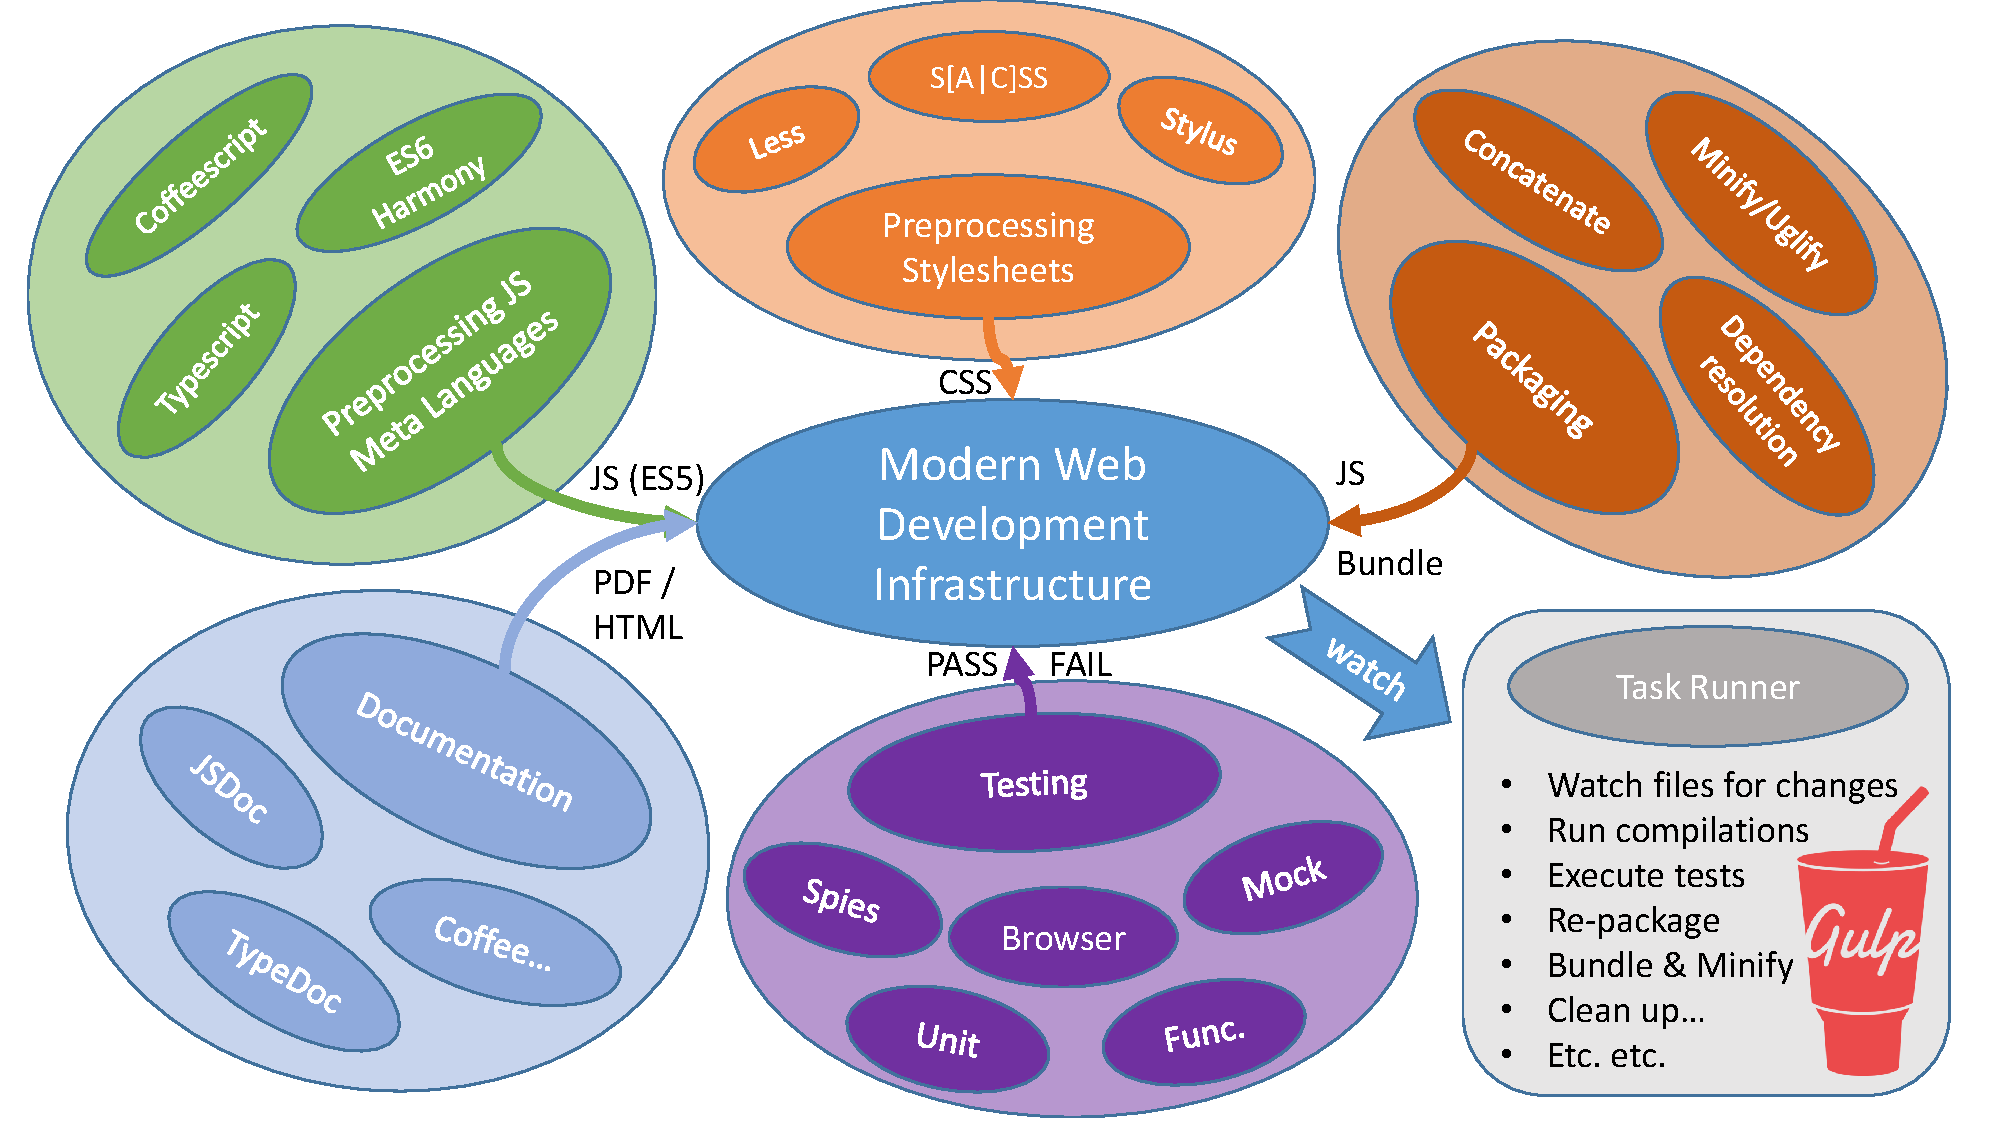
\includegraphics[width=1.8\textwidth]{figures/Modern_Web_Dev}
	\caption{Modern Web Development Component Diagram}
	\label{fig:webdev_cycle_components}
\end{figure}
\end{landscape}


\section{Graphinius JS}
\label{library}

	The components presented in this section correspond with the graphical elements in Figure~\ref{fig:webdev_cycle_components}.

	\subsection{Preprocessing (compiling) JS Meta Languages}
	\label{ssect:language}
	
		\subsubsection{Javascript / ES6}
		\label{sssect:js_es6}
		
		Although the JavaScript language was put together by Brendan Eich of the Netscape company within 3 weeks in 1994 (when it was initially called LiveScript, and in 1995 renamed to JavaScript in a marketing attempt to jump on the Java-hype bandwagon), it turned out to be a nifty little language for general in-browser development and computations. JavaScript is a prototype based language, which means that it uses pointers to parent objects instead of class instantiations, features first-order functions (functions which can generate functions) and function-as-object passing, which is ideal for callback-based implementations of the visitor pattern, even more so as JS functions are automatically closures (functions or lambdas that have, regardless of their execution context, full access to their original definition scope).
		
		After almost two decades however, the JS development community felt that requirements on modern web-based product had increased so drastically, that traditional JavaScript could only partially serve them anymore. Problems are - amongst others: 1) the lack of an explicit type system (which is crucial for larger software projects), 2) the lack of an implicit module system allowing for requiring other files or packages (except in the form of browser script tags), 3) the lack of a chaining system for async callbacks (which resulted in the notorious 'pyramid of doom'), 4) the somewhat peculiar functional scoping, which is mostly an entrance barrier to developers of other languages, as well as 5) a general lack of elegant language constructs (like deconstruction of objects into variables etc.).
		
		While some of those problems have been addressed even in the context of ECMAScript 5 (like the introduction of promises to replace nested callback functions), many shortcomings could only be addressed by external libraries, which polluted the workflow with additional dependencies not needed in more sophisticated languages and often increasing the JS download size by hundreds of kilobytes, which can become a problem on mobile devices.
		
		ECMAScript 6 (codename harmony) is an overhaul of the JavaScript language featuring classes, a new keyword for the familiar block scoping ('let'), as well as an integrated module system allowing to require external files even inside the browser. The greatest obstacle to using ES6 today is the lack of complete support across all browser vendors - this is where ES6-to-ES5 compilers like \textit{Traceur} or the more popular \textit{Babel} come in. As far as syntax goes, ES 6 cleans up some keyword usages in order to make code more readable (samples taken from \url{http://es6-features.org/}):
		
		
		\begin{lstlisting}[caption={ECMAScript 5 (usually referred to as 'JavaScript') version of functional programming using the natively built-in mapping function.}, label={fig:ECMAScript5_mapping}, language=JavaScript]
	odds  = evens.map(function (v) { return v + 1; });
	pairs = evens.map(function (v) { return { even: v, odd: v + 1 }; });
	nums  = evens.map(function (v, i) { return v + i; });
		\end{lstlisting}
		
		
		\begin{lstlisting}[caption={ECMAScript 6 equivalent to the above code.}, label={fig:ECMAScript6_mapping}, language=JavaScript]
	odds  = evens.map(v => v + 1)
	pairs = evens.map(v => ({ even: v, odd: v + 1 }))
	nums  = evens.map((v, i) => v + i)
		\end{lstlisting}
		
		Although ES6 is a great improvement over ES5 in many respects, it still lacks an explicit type system and interfaces (which can guide an IDE in it's analysis regarding Code Completion and IntelliSense). It was therefore not considered the best option for the development of a potentially large library as GraphiniusJS.			
		
		\subsubsection{Coffeescript (CS)}
		\label{sssect:coffeescript}
		
		Coffeescript was an attempt to make JavaScript code more readable as well as writable. It was apparently inspired by the clean syntax used in modern scripting languages like Ruby or Python and adopted the use of whitespace as control characters like Python (but not Ruby). Most of the language was based on using 'syntactic sugar' to abbreviate otherwise verbose JS code. For instance, the  \textit{this} variable was replaced by the  \textit{@} sign, the return statement at the end of a function became superfluous, and the lambda operator \textit{->} was introduced as a shortcut for the \textit{function} keyword in normal JS. Examples taken from \url{http://ricardo.cc/2011/06/02/10-CoffeeScript-One-Liners-to-Impress-Your-Friends.html}
		
		\begin{lstlisting}[caption={Two versions of the same mapping functionality in CoffeeScript}, label={fig:Coffeescript_mapping}, language=JavaScript]
	[1..10].map (i) -> i*2
	i * 2 for i in [1..10]
		\end{lstlisting}
		
		Like ES6, Coffeescript is compiled down to ES5 through it's own coffee compiler. As much as the idea of CS is neat and very justified for individual developers, the use of whitespace as control characters can add some additional hassles if working in a team; only slight deviations in the individual setup can cause serious problems, like the use of editors that use different representations for tabs (tab vs 2 spaces vs 4 spaces) or different line ending symbols (Windows vs. Mac vs. Linux). Furthermore, CS did not resolve the lack of an internal module system or the lack of an explicit type system, and was therefore not considered for Graphinius JS.
		
		
		\subsubsection{Typescript}
		\label{sssect:typescript}
		
		
		
		
	\subsection{Testing}
	\label{ssect:testing}
	
		\subsubsection{Jasmine}
		\label{sssect:jasmine}
		
		\subsubsection{Mocha / Chai(!)}
		\label{sssect:mocha_chai}
		
		\subsubsection{Mocking Library (Sinon)}
		\label{sssect:mocking}

		\subsubsection{Selenium(??)}
		\label{sssect:selenium}
		
	
	\subsection{Documentation}
		\label{ssect:documentation}
		
		\subsubsection{JSDoc}
		\label{sssect:jsdoc}
		
		\subsubsection{TypeDoc}
		\label{sssect:typedoc}
		

	\subsection{Build system for browser}
		\label{ssect:build_browser}
		
		\subsubsection{Browserify}
		\label{sssect:browserify}
		
		\subsubsection{request.js}
		\label{sssect:request_js}
		
		\subsubsection{webpack}
		\label{sssect:webpack}


	\subsection{Task Runner}
	\label{ssect:build_system}
	
		\subsubsection{Grunt}
		\label{sssect:grunt}
		
		\subsubsection{Gulp}
		\label{sssect:gulp}
		
		\begin{figure}[ht]
			\label{fig_grunt_gulp}
			\centering
			\hspace*{-1.4cm}
			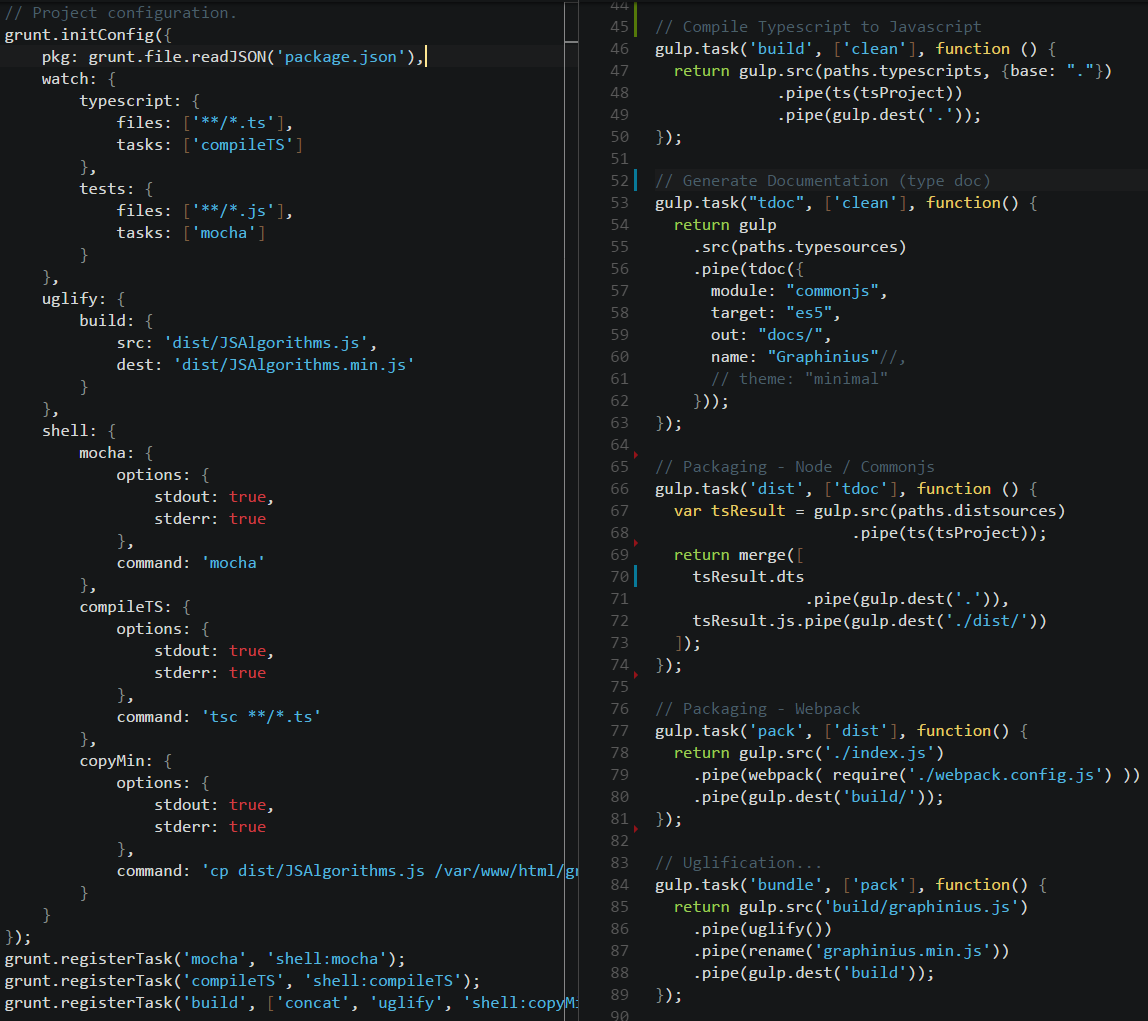
\includegraphics[width=1.2\textwidth]{figures/grunt_gulp_comparison}
			\caption{Comparison between Grunt \& Gulp build systems}
		\end{figure}
		
	






\section{Graphinius VIS}
\label{sect:graphinius_vis}

Description of Nicole's choices and decisions...

\begin{landscape}
\begin{figure}[ht]
	\label{fig_vis_control_flow}
	% \centering
	\hspace*{-1cm}
	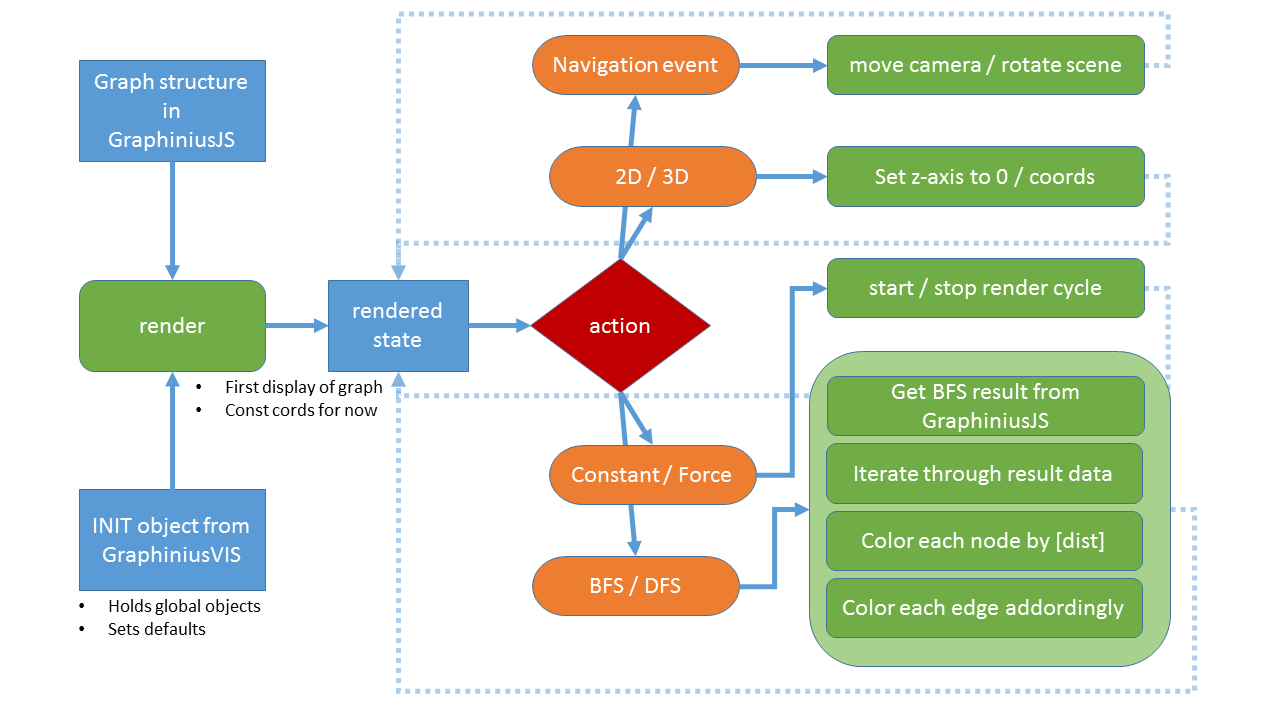
\includegraphics[width=1.9\textwidth]{figures/VIS_Control_Flow}
	\caption{Graphinius VIS control flow}
\end{figure}
\end{landscape}





\chapter{Architecture / Implementation}
\label{ch:implementation}

The Graphinius Platform consists of four main components as depicted in the following diagram. Of those 4, the practical parts of this Master thesis mainly consider Graphinius Base, with all graph construction and analysis functionality residing in GraphiniusJS. 

\begin{figure}[H]
	\centering
	\hspace*{-0.5cm}
	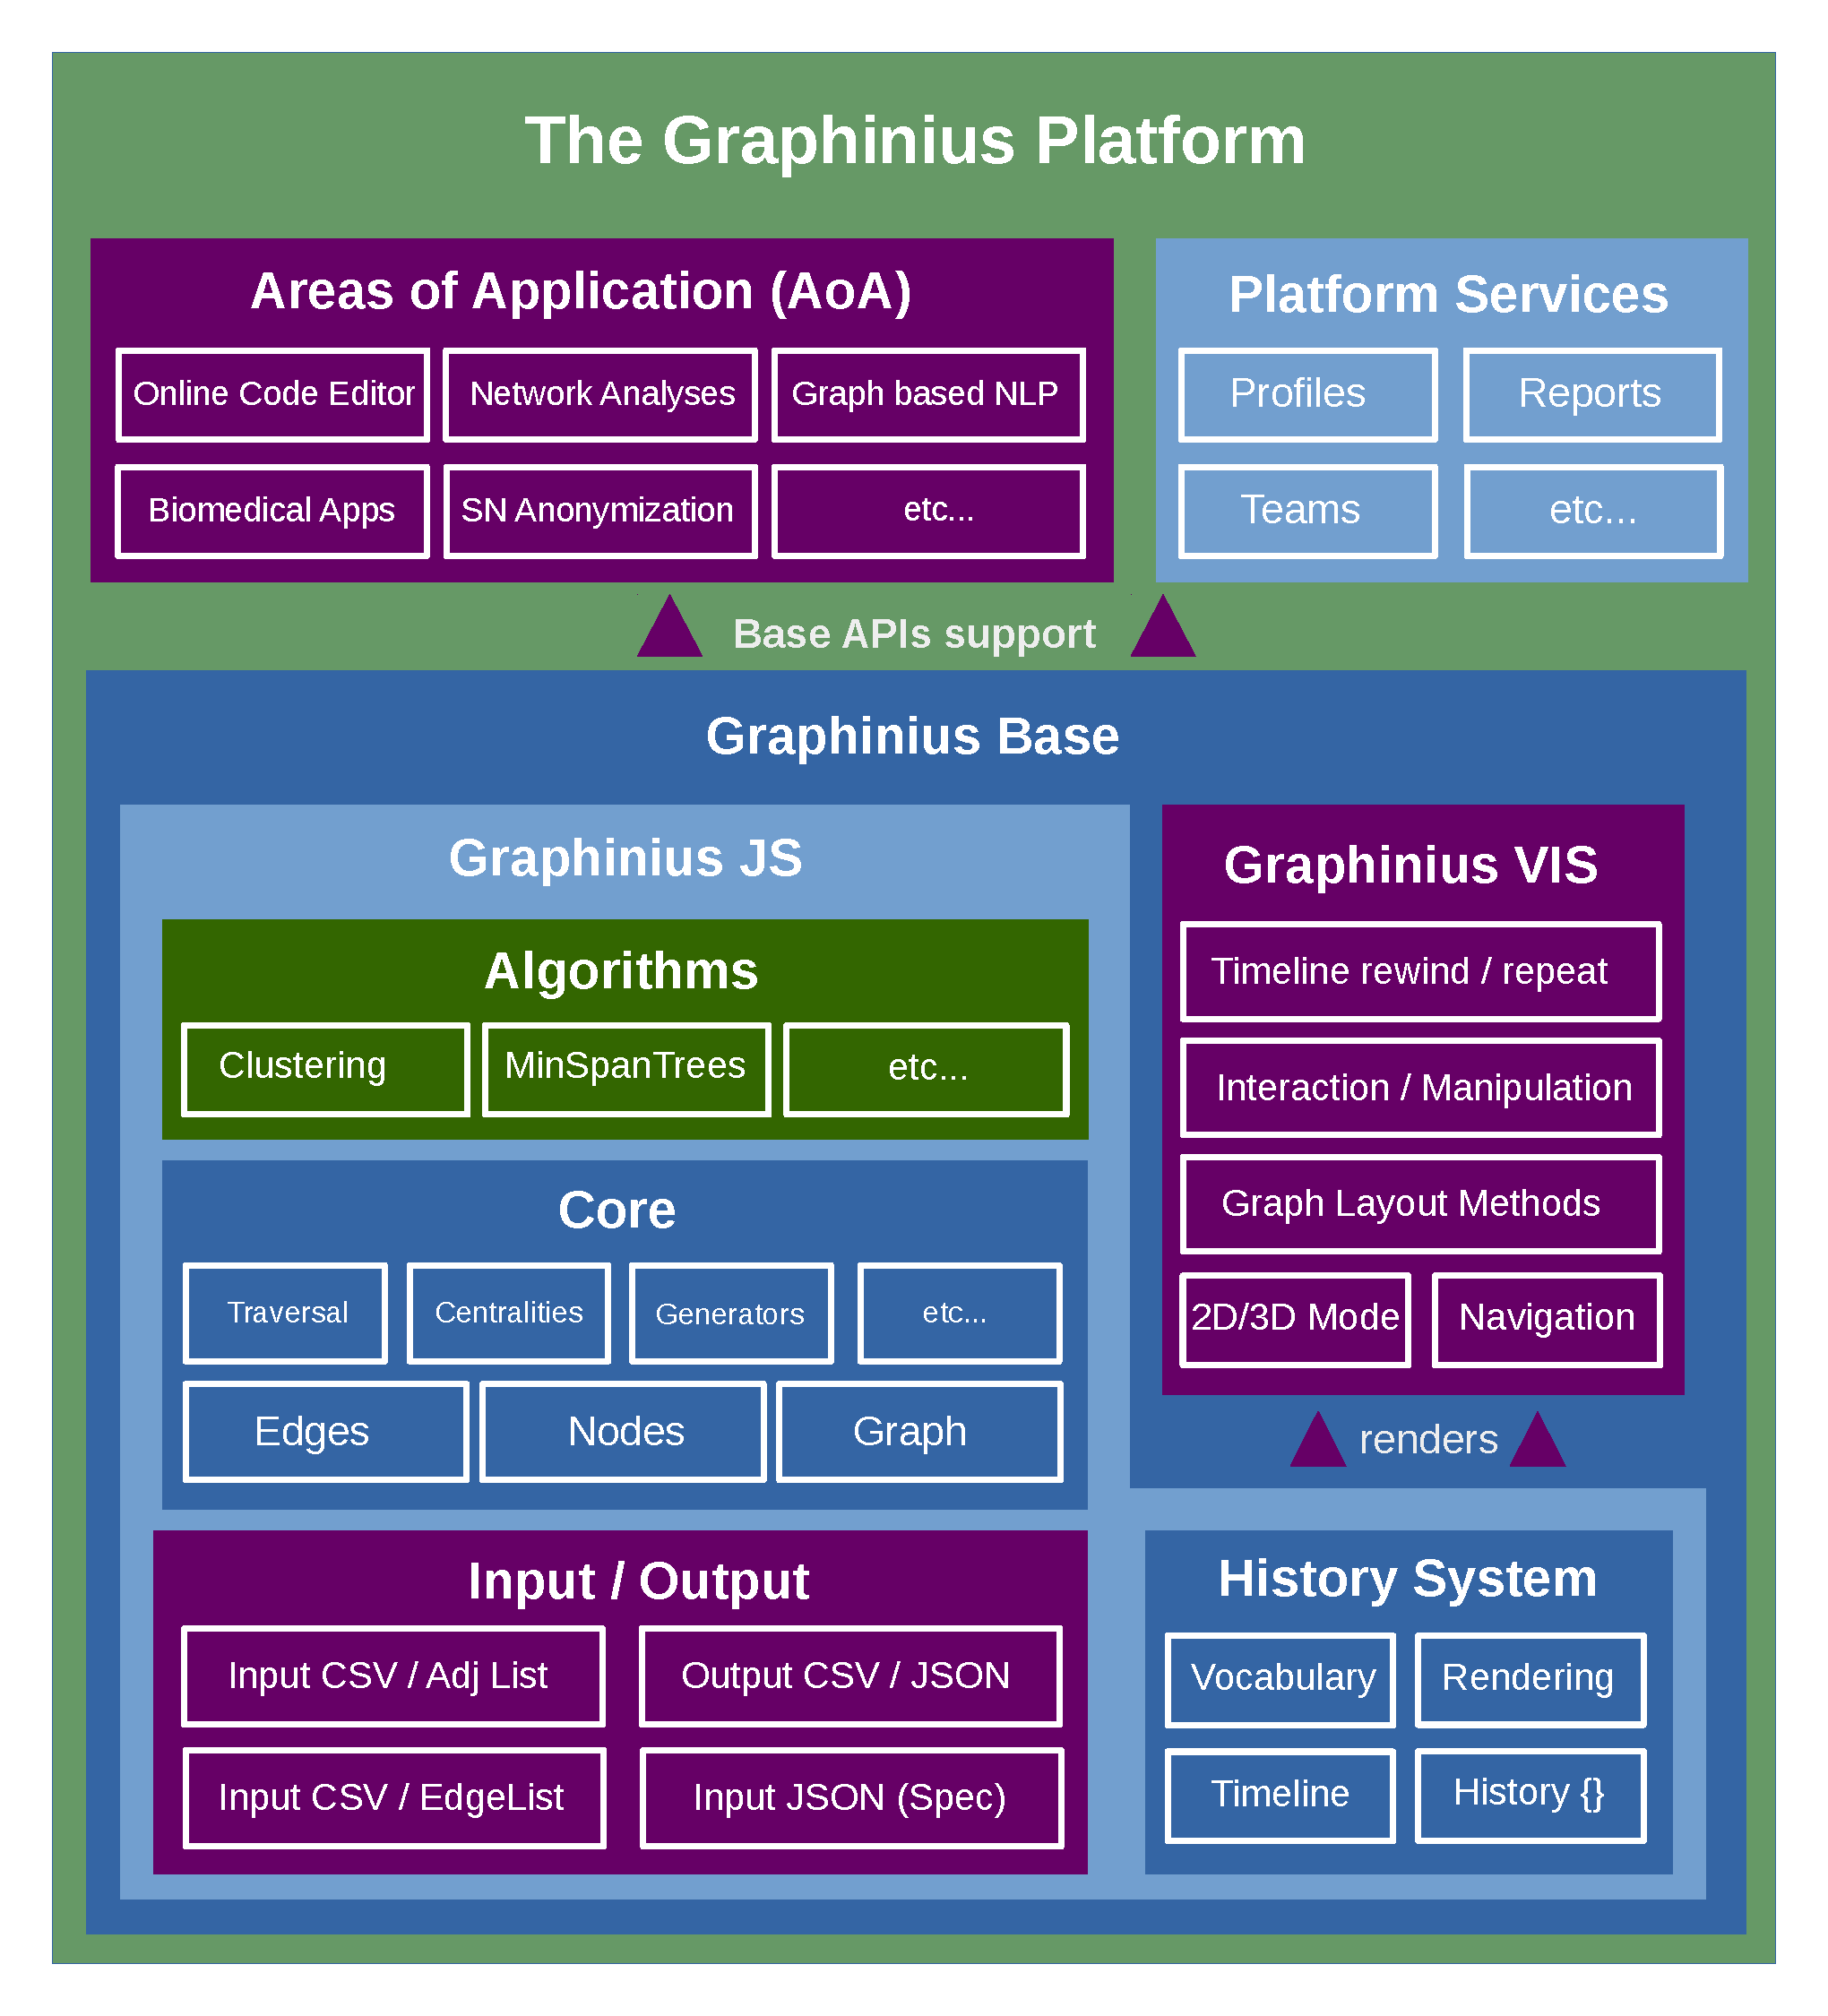
\includegraphics[width=1.05\textwidth]{figures/Graphinius_Architecture_new}
	\caption{Graphinius platform architecture overview}
	\label{fig:graphinius_architecture}
\end{figure}


\section{Graphinius Base}
\label{sect:graphinius_base}

As the name suggests, the Base module offers all the functionality necessary to develop graph-based applications on top of it, including basic graph-computations and algorithms as well as real-time, in-browser visualization. It is therefore logically composed of the two main modules \textit{GraphiniusJS} and \textit{GraphiniusVIS} as well as a mechanism of communication between those two, the \textit{History System}.

\section{Graphinius JS}
\label{sect:graphinius_js}

	Graphinius JS deals with graph loading via Input Readers for CSV and JSON file formats, instantiation as well as mutation of graphs through the graph, nodes and edge classes as well as some basic graph algorithms, including degree distributions, edge generators and traversal via breath-first, depth-first and best-first (priority-first) search algorithms. As not all components depicted in Figure~\ref{fig:graphinius_architecture} are of equal importance (or implemented yet), the following substructure does not fully comply with the organization of that diagram.
		
	\subsection{Edges}
	\label{ssection: core_edges}
	
	Edges are the most basic class within the GraphiniusJS library. They depend on the Nodes class solely in order to be able to check if their endpoints consist of valid graph nodes. Edges can never instantiate nodes themselves, so in order to add a valid edge to a graph, the connected nodes must already exist in the structure. Edges can be directed or undirected, weighted or unweighted, hold an ID and can be given a label. Apart from that, they contain no other internal logic.
	
	\subsection{Nodes}
	\label{ssection: core_nodes}
	
	Nodes are already a lot more complex in Graphinius JS. They consist of an ID, an optional label, and have datastructures to hold the directed as well as undirected edges connected to them; When adding and removing connected edges they measure and update their own degrees (according to the mixed-graph nature of Graphinius, we always differentiate between in-, out-, and undirected degree) and are the lowest-level objects used in graph traversal, as they contain the necessary functionality to return their neighboring nodes (according to outgoing, incoming, or undirected edges).
	
	\subsection{Graph}
	\label{ssection: core_graph}
	
	The Graph class is the main component at the core of Graphinius JS as it contains all necessary functionality to create as well as add and remove nodes and edges to a graph. It keeps track of its size in number of nodes and edges, holds datastructures to look up those objects as well (as always it differentiates between directed and undirected edges), can return a random node or edge, clean nodes from all incoming, outgoing or undirected edges and contains helpers to print statistics or the degree distribution over its nodes.
	
	Moreover, it contains the GraphMode setting which has two different meanings: As a metric of the graph, it tells a caller if the graph contains no edges at all (GraphMode.INIT), holds only undirected (GraphMode.UNDIRECTED) or directed (GraphMode.DIRECTED) edges, or a mixture of both (GraphMode.MIXED). As a setting for graph traversal, it enables \textit{graph views} by allowing algorithms operating on it to only see a subset of all the existing edges in the graph.
	
	\begin{lstlisting}[caption={Graph traveral dependent on GraphMode.}, label={lst:traversal_mode}, language=JavaScript]
if ( dir_mode === $G.GraphMode.MIXED ) {
	bfsScope.adj_nodes = bfsScope.current.adjNodes();
}
else if ( dir_mode === $G.GraphMode.UNDIRECTED ) {
	bfsScope.adj_nodes = bfsScope.current.connNodes();
}
else if ( dir_mode === $G.GraphMode.DIRECTED ) {
	bfsScope.adj_nodes = bfsScope.current.nextNodes();
}
else {
	bfsScope.adj_nodes = [];
}
	\end{lstlisting}
	
	
	\subsection{Edge Generators}
	\label{ssection: core_}
	
	There are many graph generators found in more established graph libraries and even specialized generator-only components (like \citep{bader2006gtgraph}), which can be used to generate random graphs or graphs following a specific layout (trees, circles, spheres, arc diagrams etc.). For the emerging GraphiniusJS library, complete graph generators were not yet considered, but edge generators implemented. This allows us to take generic point cloud data (coming from diverse sources like tabular datasets, range images etc.) and convert them into a graph structure by adding random connections according to two different approaches:
	
	\begin{itemize}
		\item \textbf{Per probability.} This algorithm goes through all node combinations in the graph and adds an edge between them with a certain probability. By its very nature, the algorithm runs in quadratic runtime in the number of nodes.
		\item \textbf{Per node.} Considering every node in sequence and adds a certain number of edges between that node and another, randomly chosen one. This algorithm could take quadratic runtime in the number of nodes (if the random node algorithm chooses so poorly that it tries to add the same edge over and over again) but in practice should perform considerably faster.
	\end{itemize}
	
	
	\subsection{Degree distribution}
	\label{ssection: core_degrees}
	
	Probably the easiest algorithm performable on a graph is to compute the degree distribution over its nodes. It simply walks over the internal node structure, counting all the ingoing, outgoing, and undirected edges returning some (numerical) histogram. The following figure depicts how to obtain a degree distribution in GraphiniusJS via a browser debugging console.
	
	\begin{figure}[H]
		\centering
		\hspace*{-0.5cm}
		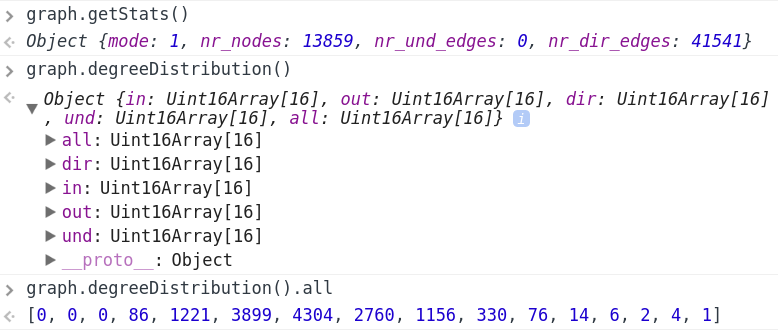
\includegraphics[width=1\textwidth]{figures/deg_dist}
		\caption{Degree distribution of a graph with 13859 nodes and 41541 edges }
		\label{fig:graphinius_architecture}
	\end{figure}
	
	
	\subsection{Graph Traversal}
	\label{ssect:search_bfs}
	
		\textit{Graph traversal} is the general term for exploring a graph from a given start node (also called 'root' node in this context). There are three basic forms of traversal differentiating by the order by which new nodes are visited. In GraphiniusJS, graph traversal is implemented using the visitor pattern by defining callback functions for specific 'hooks' in the traversal procedure. The graph traversal algorithm is thus reduced to only running its particular node-expansion scheme on the data structures necessary for its purpose; the actual information 'extraction' and result 'compilation' is then done by executing the injected callbacks at the aforementioned, pre-determined hooks. Let's take a look at an example callback initializing the result set of a Breadth first search algorithm at the start of it's invocation and pushing that callback onto the \textit{init\_bfs} callback array inside the algorithm's config.callbacks object:
		
		\begin{lstlisting}[caption={Defining a callback function for traversal.}, label={lst:traversal_cb}, language=JavaScript]
// Standard INIT callback
var initBFS = function( context : BFS_Scope ) {
// initialize all nodes to infinite distance
for ( var key in context.nodes ) {
	config.result[key] = {
		distance : Number.POSITIVE_INFINITY,
		parent 	 : null,
		counter	 : -1
	};
}
callbacks.init_bfs.push( initBFS );
		\end{lstlisting}
		
		During the actual BFS run, this callback is then executed as follows:
		
		\begin{lstlisting}[caption={Executing a callback function during traversal.}, label={lst:traversal_cb_exec}, language=JavaScript]
// Execute INIT callback
if ( callbacks.init_bfs ) {
	$CB.execCallbacks(callbacks.init_bfs, bfsScope);
}
		\end{lstlisting}

	
		\subsubsection{Breadth first search}
		\label{sssect:search_bfs}
		
		BFS traverses a graph by expanding one 'shell' of nodes after the other, which means that it progresses outwards from a starting node like the layers of an onion until all reachable nodes have been visited. It is primarily used for getting a sense of distances in a graph (although it does not compute shortest paths by itself) and uses a queue datastructure to add nodes it's list of future visitations.
		
		In GraphiniusJS, BFS makes use of the following hooks: 1) \textbf{init\_bfs} at the start of the algorithm, 2) \textbf{node\_unmarked} when an encountered node has not yet been marked as visited, 3) \textbf{node\_marked} in case such a node has already been visited, and 4) \textbf{sort\_nodes} in the case the user wants to imply a certain order by which to add nodes to the queue - this does not change the nature of BFS, however.
		
		\subsubsection{Depth first search}
		\label{sssect:search_dfs}
		
		DFS explores new nodes in a recursive fashion, which makes it advance 'deep' into the far reaches of the graph structure before exploring the immediate vicinity of the start node. For this purpose it uses a stack as its basic datastructure; moreover, if no more nodes are reachable from a given departure node, but the graph structure has not been entirely explored yet, DFS (via an outer loop) will randomly choose one of the remaining nodes, thereby arriving at a (random) segmentation of the entire graph.
		
		In GraphiniusJS, DFS provides the following hooks: 1) \textbf{init\_dfs} at the start of the outer loop, 2) \textbf{init\_dfs\_visit} at the start of a 'visit' (the inner loop), 3) \textbf{node\_popped} for any callbacks to execute directly after a node has been taken from the stack, 4) \textbf{node\_marked} which behaves as in BFS, 5) \textbf{node\_unmarked} which behaves as in BFS, 6) \textbf{sort\_nodes} which behaves as in BFS, and 7) \textbf{adj\_nodes\_pushed} which executes directly after a node has been expanded and its neighbors pushed to the stack.
		
		\subsubsection{Best (priority) first search}
		\label{sssect:search_pfs}
		
		PFS always picks from its available nodes the one that evaluates to an optimal value (e.g. the minimal distance given an edge weight) - it therefore uses a (MIN / MAX) heap as its underlying datastructure, which in GraphiniusJS has been implemented with injectable heuristics (via callback functions as described in the Graph Traversal~\ref{ssect:search_bfs} section).
		
		PFS lets the caller inject the following callbacks: 1) \textbf{init\_pfs} is invoked at the start of the algorithm, 2) \textbf{node\_open} in case an encountered node is already contained in the OPEN set, 3) \textbf{node\_closed} in case an encountered node is already contained in the CLOSED set, 4) \textbf{better\_path} in case a more optimal path to a node under test has been discovered, and 5) \textbf{goal\_reached} if we have encountered a specified end goal causing the algorithm to immediately return.
		
	\subsection{Traversal-based algorithms}
	\label{ssect:travseral_algos}
	
	Although as of the time of this writing, no more algorithms have been implemented in Graphinius JS, most of the commonly used techniques are building upon one or the other form of basic graph traversal. This includes shortest paths, cycle testing, topological sorting of nodes, strongly connected component analysis, minimum spanning trees, some centralities (closeness and betweenness for instance) as well as many more than the author (or reader) will be able to recollect.
	
	Building all traversal-based algorithms on top of either BFS, DFS or PFS utilizing their callback \& hook structure will enable us to easily add new graph-views defined on node or edge types (and other criteria) to the library in the future, without having to re-adapt each and every single component to the respective improvement.

	
	\subsection{Input / Output}
	\label{ssect:input_output}
	
	There are two basic input readers implemented in GraphiniusJS: 
	
	\textbf{The CSV Reader}, which takes adjacency lists or edge lists in CSV format and supports the most simple, but widely used, formats as well a a few additional options, and
	\textbf{The JSON Reader}, which operates on a custom, Graphinius-related JSON file format in order to support additional features specific to the use cases of the platform.
	
	As of the time of this writing, standard output filters have not been implemented, but would follow the same principles outlined below for their input counterparts.
		
		
		\subsubsection{CSV Reader}
		\label{sssection: io_csv}
		
		The CSV Reader class supports to widely used graph representation formats, namely \textit{adjacency lists} and \textit{edge lists}. An adjacency list is usually composed of lines indicating a StartNode at position one, followed by a series of connected EndNodes at the following positions in the line, where the connections can be interpreted as either directed or undirected edges:
		
		\begin{lstlisting}[caption={Sample Adjacency list, no edge direction.}, label={lst:adj_list_nodir}, language=JavaScript]
		A, B, C, A, D
		B, A
		C, A
		D, A
		\end{lstlisting}
		
		In addition to that, the Graphinius CSV Reader can be configured to consider explicitly defined edge directions, as in the following listing, or instructed to interpret all edges as either directed or undirected regardless of the direction specified in a file.
		
		\begin{lstlisting}[caption={Sample Adjacency list including edge direction.}, label={lst:adj_list_dir}, language=JavaScript]
		A, B, u, C, u, A, d, B, d, D, d
		B, A, u
		C, A, u, A, d
		D, A, d
		\end{lstlisting}
		
		CSV Edge Lists work analogously but are even simpler and use the format \textit{(StartNode, EndNode [,directed])}.	
		
		
		\subsubsection{JSON reader}
		\label{sssection: io_json}
		
		The Graphinius JSON reader is a more complex class as it uses it's own data format specific to the use cases targeted by the platform. It uses a nested object structure defining an array of node objects potentially containing different arrays of sub-objects:
		
		An \textbf{edge array} containing objects specifying a \textit{to} node, a \textit{direction} specifier as well as some \textit{weight}; direction and weight are optional; a \textbf{coordinates} array containing the \textit{x}, \textit{y}, and \textit{z} coordinates of a node; the \textit{z} coordinate is optional; a \textbf{feature vector} containing a hashmap of arbitrary length containing objects of arbitrary type including nested structures. The feature vector is solely used by applications building on GraphiniusJS and ignored by the standard suite of algorithms as described in the previous section. A sample of a valid graph in the Graphinius JSON file format is depicted in Figure~\ref{fig:json_input_graph}.
		
		\begin{figure}[ht]
			\centering
			\hspace*{-1.5cm}
			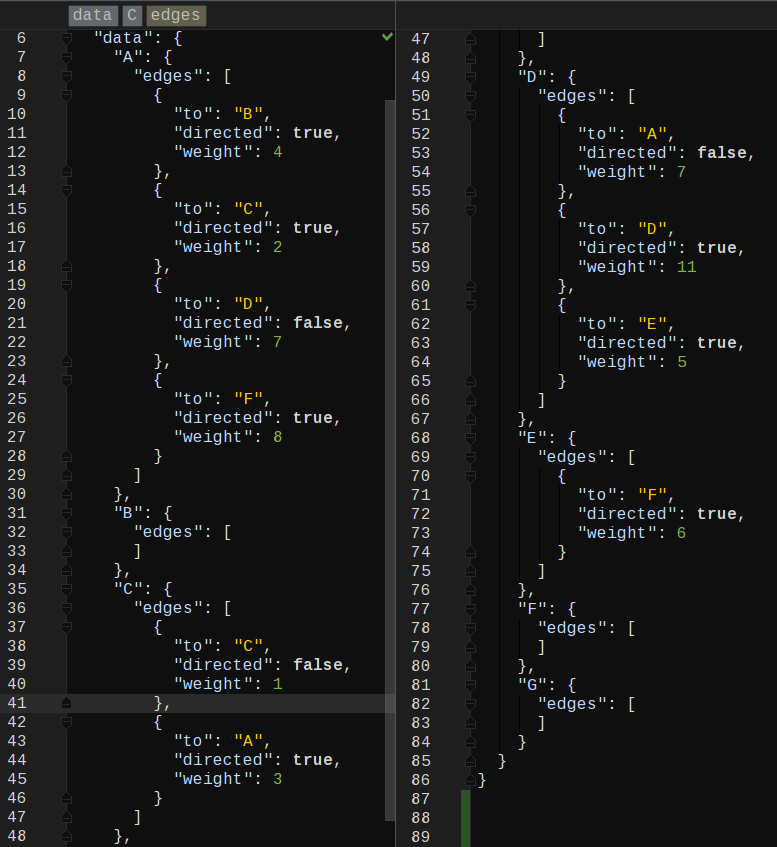
\includegraphics[width=1.2\textwidth]{figures/search_graph_json}
			\caption{Sample graph in the Graphinius JSON format}
			\label{fig:json_input_graph}
			\small Apart from the 'to' node, direction and weight, any node can exhibit an arbitrarily large feature vector containing any type of information (like patient data, word vectors, etc.). Another special sub-object which the input reader is looking for is the 'coords' object, which specifies the coordinates used in the constant layout renderer of the GraphiniusVIS library.
		\end{figure}



\section{The History system}
\label{sect:op_log}

	The idea of a history subsystem came from the concept of a real-time in-browser graph exploration platform, in which every action performed via an online editor or some GUI action should result in some immediate, visible change in the graph visualization. Ideally, such real-time changes would also be reversible, so that a user could progress step-by-step forward and backward in time - either to grasp more clearly what some algorithm does to the structure of a graph, or to 'simulate' the behavior of an algorithm on the whole. 
	
	In order to guarantee smooth behavior as well as separation of concerns in the software, placing this functionality directly in either the GraphiniusJS or GraphiniusVIS libraries would violate sound architectural principles. Therefor, the author proposes (but has not implemented yet) the following general module:
	
	\begin{landscape}
		\begin{figure}[ht]
			\label{fig_history_workflow}
			\centering
			\vspace{-2.0cm}
			%	\hspace*{0cm}
			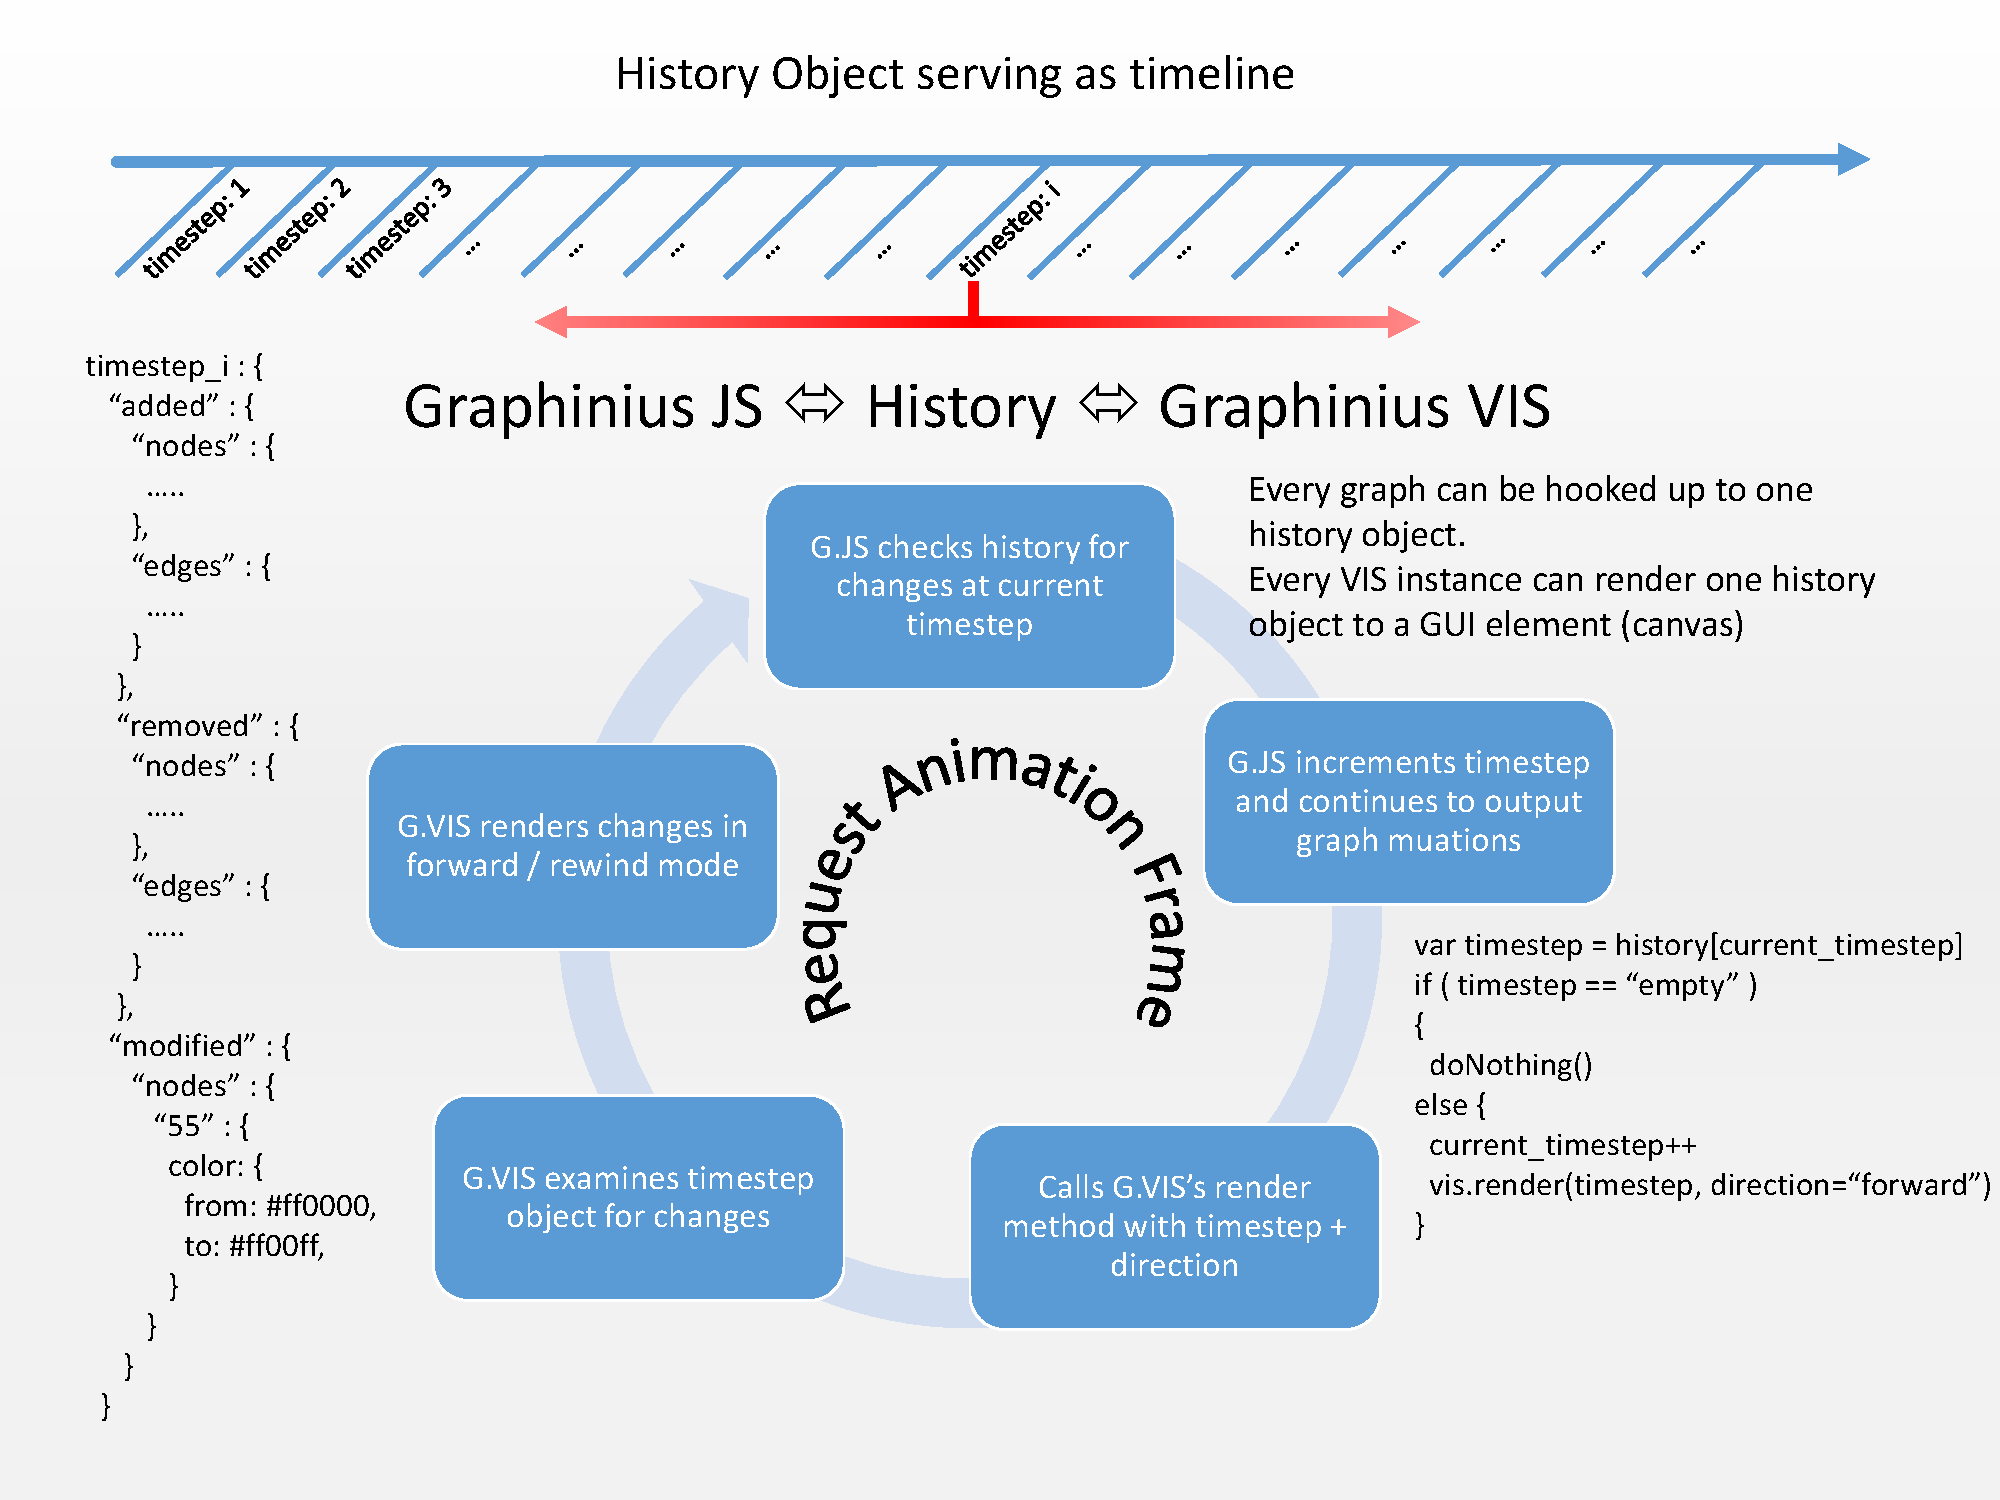
\includegraphics[width=1.6\textwidth]{figures/History_Workflow_pdf}
			\caption{Graphinius JS <-> VIS communication via Op-Log}
		\end{figure}
	\end{landscape}

	\subsection{Timeline}
	\label{ssect:timeline}
	
	The basic idea in implementing the system is to organize all graph mutations along the time axis, if only to imply chronological order. While it is less important to be able to specifically 'audit' some action in the sense of being able to exactly locate its temporal occurrence, we need some mapping of actions to a timestep (object) in order to be able to traverse the timeline back and forth. This is what determines the structure of the history object.
	
	\subsection{History Object}
	\label{ssect:history_object}

	The history object is a simple JavaScript object (which behaves like a hashmap in other languages' vocabulary) and holds entries in the form of \textit{timestep(timestep:number => actions:JSObject)}. These actions sub-objects then contain all the mutations which took place at a certain \textit{timestep}. It is important to realize that this \textit{timestep} is not an exact moment in time, but can span an arbitrarily long interval. Its value is determined by a global \textit{timestep} variable, which is only incremented when the rendering of the currently 'active' timestep has commenced. The actual procedure take the form of the following loop:
	
	\begin{enumerate}
		\item Graphinius Platforms runs recursive calls to \textit{window.requestAnimationFrame(renderFunc)} which simulates a main GUI loop
		\item At the beginning of each invocation, the algorithm checks for the current value of the global \textit{timestep} variable, and checks if the respective entry in the history object is empty or populated.
		\item In case it is empty, the algorithm breaks, laying inactive until the next time-tick from requestAnimationFrame (16.67 milliseconds on a 60Hz monitor).
		\item In case it is populated, the algorithm increments the global \textit{timestep} value - from this point onwards, GraphiniusJS will not write to that entry any more ('locking' it so that the rendering process can finish).
		\item All items in the current \textit{timestep} object will be evaluated resulting in calls to the GraphiniusVIS library updating the in-browser visualization.
	\end{enumerate}
	
	In order to be able to replay / rewind the mechanism, the history subsystem must have a sense of direction in time - which in our case simply translates to possessing a vocabulary expressing graph mutations in such a way that the respective inverse function is easily obtainable.
	
	\subsection{Vocabulary}
	\label{ssect:vocabulary}
	
	In order to achieve this, the \textit{timestep} entries must be as simple and specific as possible. For most of the primitive graph mutations, this is practically going to happen automatically: For instance, given the command \textit{'addNode(nodeId, arguments)'}, the inverse is logically \textit{'deleteNode(nodeId)'}. For more complex actions like changing coordinates, colors or shape, the original values would have to be stored. In the case of actions regarding whole clusters or changing the structure of the entire graph (\textit{run mincut..}), the \textit{timestep} entries will have to be broken down into atomic units and inverse actions defined in beforehand.


\section{Graphinius VIS}
\label{sect:graphinius_vis}

	The author was fortunate to receive the opportunity to guide the Master's Project of Nicole Neuhold in implementing a visualization module for the emerging Graphinius platform. We were working on research, experiments, and the foundation of a future implementation from early January 2016 to the end of March of the same year, and I am proud to be able to say that we surpassed our initial expectations - in brevity and conciseness of implementation as well as performance - by leaps and bounds and are not able to visualize graphs of 15k nodes / 40k edges fluently (~25 FPS) even on middle class laptops (22k nodes / 65k edges fluently on the author's desktop machine featuring a low-middle-class Geforce 650TI with 2GB of video RAM).
	
	\subsection{WebGL rendering}
	\label{ssect:webgl_rendering}
	
	The core component of the GraphiniusVIS module is the WebGL renderer. Although we experimented with SVG and Canvas (2D) as well, we quickly realized that both alternatives were either too slow or didn't provide us with the experience we desired: SVG has the great advantage of working with normal browser (DOM) objects, which enables easy interaction and selection via JS / CSS selectors, but stops rendering fluently at only a few hundred nodes / a few thousand edges.
	
	Canvas, on the other hand, is fine and fast enough for visualizing logical graph structures of thousands of nodes / edges in 2D. Nevertheless, because our project originated from the need to render structures  inherently 3D (like nevi and organs) and there was no easy possibility to project a 3D space onto a 2D canvas (except for computing the projection ourselves), we finally decided against it.
	
	Our Three.js / WebGL based renderer now uses low-level data structures like buffer geometries, statically typed JavaScript arrays and particle systems instead of 3D objects for nodes, which enables us to transfer our (pre-)computed data to the GPU in one single copy operation - this alone increases performance easily 10-fold over earlier attempts at progressively adding new objects to the scene.
	
	\subsection{2D/3D Mode}
	\label{ssect:vis_2d3d}
	
	GraphiniusVIS supports both 2D and 3D visualization of graph structures. However, since we are using WebGL which is inherently 3D, when switching to 2D mode we are not falling back to SVG or canvas but instead just 'fix' all z-coordinates of nodes / edges to zero, so we end up with a 2D object floating in 3D space.
	
	\subsection{Navigation}
	\label{ssect:vis_navigation}
	
	Our module supports panning (via mouse click-and-move), zooming (via mouse-wheel), rotating (via Shift + mouse click-and-move), and also provides any of those actions via keyboard commands.
	
	\subsection{Graph Layouts}
	\label{ssect:vis_layouts}
	
	The field of graph drawing has been an active area of research for several decades now, and many graph layouts have been developed for diverse areas of applications. Apart from constant (coordinate-based) layouts and force-directed layouts for physical simulations, there exist circular, spherical, tree-based, and arc diagrams, to name only a tiny fraction. Our basic implementation supports a constant layout per default, and allows switching to a force-directed layout as well, although the latter is currently implemented as a simple mathematical sine function instead of making use of attracting / repulsive forces.
	
	\subsection{Interaction / Manipulation}
	\label{ssect:vis_interact_manipulate}
	
	There are almost endless possibilities to interact with and manipulate a graph structure, so we were limited to offering just a small selection in order to demonstrate the viability of our GraphiniusVIS module. We chose to implement node and edge addition as well as deletion, changing the color of nodes and edges, updating their coordinates as well as switching from constant to our (simplified) force-directed layout. 
	
	In addition to that, in order to demonstrate seemless interaction (without a history object for now) between GraphiniusJS and GraphiniusVIS, one can visualize distances computed by BFS as well as segments computed by DFS (on a directed graph) from any random or chosen node. This even works during constant re-rendering in force-directed mode, although the algorithm is not yet implemented as a background thread (WebWorker / WebAssembly) and therefore causes the animation to lag for a fraction of a second.
	
	The following diagram summarizes some demo interactions / control flows contained in our base implementation.
	
	%\begin{landscape}
		\begin{figure}[ht]
			% \centering
			\hspace*{-1.3cm}
			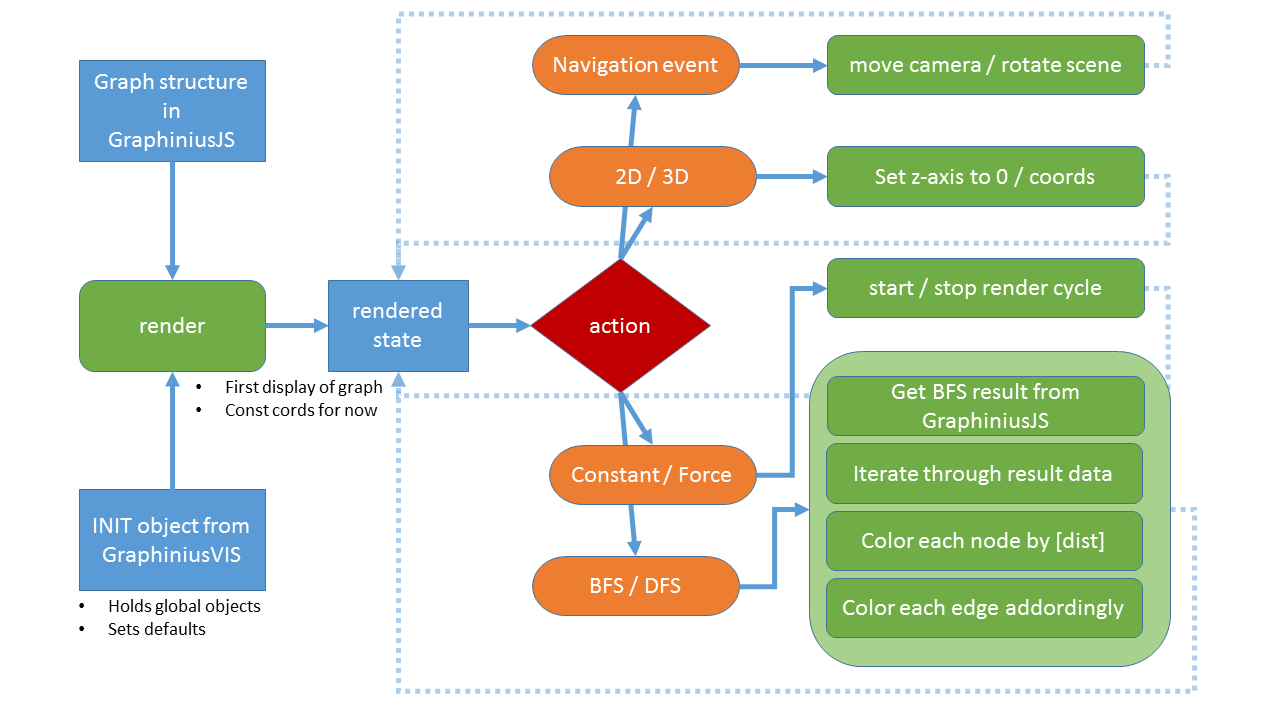
\includegraphics[width=1.2\textwidth]{figures/VIS_Control_Flow}
			\caption{Graphinius VIS control flow}
			\label{fig_vis_control_flow}
		\end{figure}
	%\end{landscape}


\section{Dependent Libraries}
\label{sect:dep_libraries}

	As described in the last chapter~\ref{ch:software_requirements}, modern web development processes utilize a wealth of external modules and helpers to achieve a seamless, convenient development workflow. Whereas GraphiniusJS does not depend on any external libraries at runtime (as can be seen in the \textit{"dependencies"} section of Figure~\ref{fig:dependencies}), the author has been using a diverse collection of dependencies at development time, which shall be only introduced in all brevity:
	
	The \textbf{chai} library handles assertions in mocha tests, \textbf{gulp} is the main taskrunner library, \textbf{gulp-clean} provides for deletion of compilation- and other results, \textbf{gulp-concat} manages file concatenations, \textbf{gulp-istanbul} integrates istanbul into the gulp process, \textbf{gulp-mocha} integrates mocha into the gulp process, \textbf{gulp-rename} handles renaming of one or many sources to a single destination file, \textbf{gulp-typedoc} integrates typedoc into the gulp process, \textbf{gulp-uglify} integrates uglify into the gulp process, \textbf{gulp-watch} provides file watching capabilities, \textbf{istanbul} provides test coverage reports, \textbf{jsdom} simulates a DOM environment in pure JavaScript (NodeJS), \textbf{jsdom-global} provides global variable support for jsdom, \textbf{json-loader} is a submodule of webpack allowing for integration of JSON files into a minified JS bundle, \textbf{merge2} merges file contents, \textbf{mocha} is the main test runner, \textbf{sinon} provides spies and stubs for testing, \textbf{sinon-chai} integrates sinon with the chai assertion library, \textbf{typedoc} automatically generates documentation from Typescript sources, \textbf{webpack-stream} is necessary for running a webpack process inside a (stream-based) gulp task, and \textbf{xhr-mock} provides a mocking service for simulating browser-based XMLHTTPRequest objects in server-side NodeJS.

	\begin{figure}[H]
		\centering
		\hspace*{-0.5cm}
		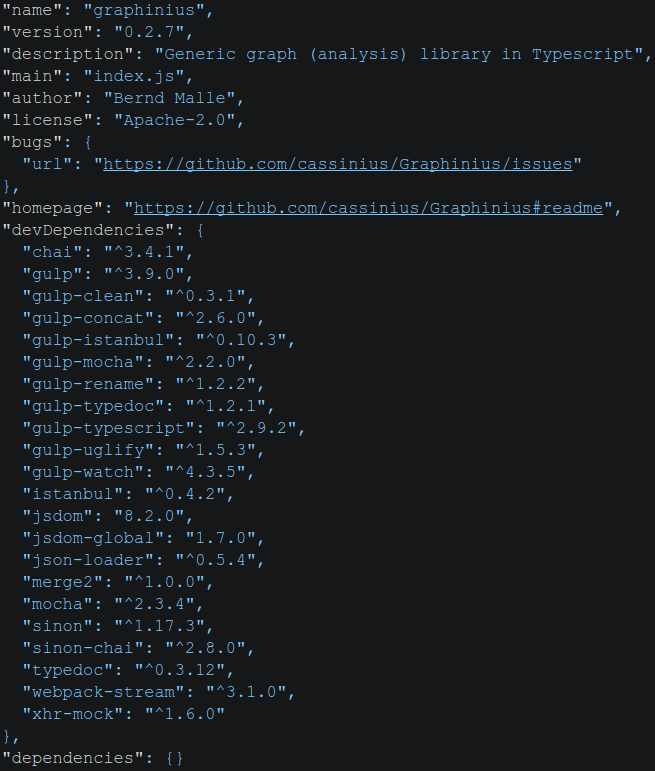
\includegraphics[width=1\textwidth]{figures/package_deps}
		\caption{GraphiniusJS development and runtime dependencies}
		\label{fig:dependencies}
	\end{figure}
	\small
	As is clearly visible, I focused on managing all complexity during development time, resulting in zero dependencies for the runtime JS bundle.


\section{Testing approach}
\label{sect:testing_approach}

	Behavior Driven Development (BDD) is a testing philosophy that approaches the development of a new feature from a high level view on the expected end-result and then works it's way down from spec's through functional to unit tests, until the feature is fully implemented, tested and covered. The ideal methodology would consist of the following steps:
	
	\begin{enumerate}
		\item Define the expected behavior of a feature (=module) in a form that both clients as well as developers understand and formulate them using (executable) specifications. The Cucumber framework introduced in the last chapter is an ideal candidate for this high level of abstraction. Executing the spec immediately will naturally fail because no code was actually written.
		\item From the specs defined in step one, we then derive functional tests which span the execution of several functions or methods in sequence in order to produce a certain result. Again, any test execution will expectedly fail as we have still not written the code yet.
		\item From the functional tests defined in step two, we finally derive low-level tests covering single units of code. Once more the tests will fail initially, upon which we endeavor to fill in the single pieces of code until all tests at that level are passing.
		\item Once the unit-test level is done, we work our way upwards to the next functional test on our todo-list. This process is repeated until all functional tests required for our initially specified features are covered.
		\item We then move on to the next feature on our product requirements list.
	\end{enumerate}
	
	 As already mentioned, because a software library intended to be used by other programmers usually has only technical clients, feature specification (testing) was omitted in programming Graphinius JS. For this reason, we will only take a look at unit and functional tests in this section (as well was mocking and spying). Furthermore, in developing a web application using the Mocha and Chai test libraries, there is no fundamental difference between unit and functional tests. Let us therefore take a look at instances of both categories to see how we would structure our approach:
	
	\subsection{Unit tests}
	\label{ssect:unittests}
	
	As stated, unit tests cover the low-level constructs of functions or methods which themselves do not depend on any lower-level functions.
	
	In the example below, we see two test cases: the first calls a binary Heap evalInputPriority function on line 2, whose job it is to cast any input to a (sortable) number, if possible. As the string "55" can be cast to the number 55, this test will be successful. In the second example on lines 5 and 6, we pass boolean values which - employing the JS \textit{parseInt(arg)} function - will evaluate to NaN (which is JS shorthand for \textit{Not a Number}).
	
	\begin{lstlisting}[caption={Unit tests covering the functionality of one simple function.}, label={fig:unit_tests}, language=JavaScript]	
it('should accept String encoded Integers as input and evaluate to their Integer value', () => {
	expect(binHeap.evalInputPriority("55")).to.equal(55);
});
it('should not accept booleans as input values (makes no sense...) ', () => {
	expect(binHeap.evalInputPriority(true)).to.be.NaN;
	expect(binHeap.evalInputPriority(false)).to.be.NaN;
});
	\end{lstlisting}
	\small
	(Sample taken from the GraphiniusJS binaryHeapTests.ts file.)
	
	
	\subsection{Functional tests}
	\label{ssect:func_tests}
	
	In functional testing we invoke some procedure which in turn will call other functions or methods, in any sequence or call depth required in order to fulfill its purpose.
	
	In the example below, we instantiate a new JSON reader, specify some configuration options and hand it a JSON file. We then expect the resulting graph to be of a certain size in number of nodes and edges. The \textit{readFromJSONFile} function will itself call several subordinate functions for reading a file from disk, processing the character sequence it receives, instantiating a GraphiniusJS graph object etc.
	
	\begin{lstlisting}[caption={A functional test covering the whole instantiation process of a graph from a JSON input structure.}, label={fig:functional_test}, language=JavaScript]
it('should correctly generate our small example graph out of a JSON file with direction _mode set to undirected', () => {
	json = new JSON_IN();
	json._explicit_direction = false;
	json._direction = false;
	graph = json.readFromJSONFile(small_graph);
	expect(graph.nrNodes()).to.equal(4);
	expect(graph.nrDirEdges()).to.equal(0);
	expect(graph.nrUndEdges()).to.equal(4);
});
	\end{lstlisting}
	\small
	(Sample taken from the GraphiniusJS JSONInputTests.ts file.)
	
	
	\subsection{Mocks used for browser code testing}
	\label{ssect:mocks}
	
	Mocks are a useful construct for testing functionality that would involve some non-trivial behavior. For instance, if we would like to test a snippet of code (as in the following code example) which loads a JSON file remotely over the network before instantiating a graph, we are assuming the existence of a server, the existence of the remote file, as well as a working Internet connection. Moreover, in this specific case, the code under test is also meant to be executed inside a browser environment, whereas we would like to invoke our test from the NodeJS console.
	
	The solution to this problem is to \text{mock} the XMLHTTPRequest object used by a browser to send AJAX requests over the internet, which - again in this specific case - replaces the object with a NodeJS request object and simulates the original XMLHTTPRequest API through a delegating wrapper around it. The exact sequence in this example is: 1) requiring the mocking library on line 3, 2) initializing a browser environment (providing the window and document objects) on line 4, 3) injecting browser globals into the Node environment on line 13, 4) requiring filesystem capabilities for local file loading on line 16 as well as loading the file on line 17, 5) initiating the mock on line 20 and finally setting up a fake web server responding to a certain URL on lines 23 through 30. The rest of the procedure (not shown in this exmaple) behaves exactly as an equivalent test inside a browser environment would.
	
	\begin{lstlisting}[caption={A mocking setup simulating a Web Server GET response...}, label={fig:mock_service_test}, language=JavaScript]
describe('Loading graphs in simulated browser environment', () => {		
	// Mocking the XHR object
	var mock = require('xhr-mock');
	var jsDomCleanup = null,
	mocked = false;
	
	// URL to replace with path
	var small_graph_url = REMOTE_HOST + "small_graph.json";
	var small_graph_path = 'test/input/test_data/small_graph.json';
	
	beforeEach(() => {		
		// Injecting browser globals into our Node environment
		jsDomCleanup = require('jsdom-global')();
		
		// Access to local filesystem for mocking service
		var fs = require('fs');
		var json = fs.readFileSync(small_graph_path).toString();
		
		//replace the real XHR object with the mock XHR object
		mock.setup();
	
		// Mocking Browser GET request to test server
			mock.get(small_graph_url, function(req, res) {
				mocked = true;
				return res
					.status(200)
					.header('Content-Type', 'application/json')
					.body(json);
			});
		});
		
	afterEach(() => {
		mock.teardown();
		jsDomCleanup();
		mocked = false;
	});
	
	// Rest of tests are the same as in non-mocked, local reader based input tests
});
	\end{lstlisting}
	\small
	... to an XML-HTTP GET Request in order to read a graph structure from a remote JSON file from inside a browser environment. (Sample taken from the GraphiniusJS JSONInputAsyncTests.ts file.)
	
	
	\subsection{Stubs}
	\label{ssect:stubs}
	There is another concept often confused with mocks called \textit{stubs}. Stubs are used when the response of a function is not supposed to be complex but rather boolean in nature. E.g. an authorization module could internally use a method checking if a user has sufficient permissions to be allowed to access a resource. This functionality could be implemented rather simply, or it could invoke elaborate tests involving diverse software modules throughout the whole system. For testing some function building upon it however, only the distinction between \textit{allowed} and \textit{not allowed} is are really of interest. Therefore, a stub can be instantiated and told to forgo any \textit{real} authority checks but instead simply return a true or false value. 
	
	The difference between stubs and mocks is therefore that stubs replace potentially complex implementations with trivial ones, whereas mocks can act as a proxy but do not necessarily reduce complexity - reading a graph from a local file is as complex as reading it from a remote one (not considering the underlying complexity of the network stack, of course).
	

	\subsection{Spies (Sinon)}
	\label{ssect:spies}
	
	Spies are test wrapper objects that observe the original function or method and record any activity regarding it, e.g. how often it was called, which argument values it was called with, which values were returned or if an error was thrown. In the example below, we instantiate a local backup object \textit{original}, then instantiate a spy on line 10, store the original function reference in our backup object on line 12, and replace the original function with our spy on line 14. In calling \$DFS.prepareDFSVisitStandardConfig on line 25, we expect to see the original function invoked in the process, which we check on line 28. The \textit{after} block from lines 18 through 21 then restores the original objects.
	
	\begin{lstlisting}[caption={A functional test making use of a spy...}, label={fig:spy_test}, language=JavaScript]
describe('testing config preparation functions - ', () => {
	var prepForDFSVisitSpy,
	prepForDFSSpy,
	original = {
		prepareDFSStandardConfig: null,
		prepareDFSVisitStandardConfig: null
	};

	before(() => {
		prepForDFSSpy = sinon.spy($DFS.prepareDFSStandardConfig);
		prepForDFSVisitSpy = sinon.spy($DFS.prepareDFSVisitStandardConfig);
		original.prepareDFSStandardConfig = $DFS.prepareDFSStandardConfig;
		original.prepareDFSVisitStandardConfig = $DFS.prepareDFSVisitStandardConfig;
		$DFS.prepareDFSStandardConfig = prepForDFSSpy;
		$DFS.prepareDFSVisitStandardConfig = prepForDFSVisitSpy;
	});

	after(() => {
		$DFS.prepareDFSStandardConfig = original.prepareDFSStandardConfig;      
		$DFS.prepareDFSVisitStandardConfig = original.prepareDFSVisitStandardConfig;
	});


	it('preprareDFSVisitStandardConfig should correctly instantiate a DFSConfig object', () => {
		var config = $DFS.prepareDFSVisitStandardConfig();
		
		// Here the spy is finally used to check internal method invocation
		expect(prepForDFSVisitSpy).to.have.been.calledOnce;
	});
});
	\end{lstlisting}
	\small
	... to test internal method invocation, restoring the original method afterwards. (Sample taken from the GraphiniusJS DFSTests.ts file.)

	
\section{Areas of Application}
\label{sect:aoas}

The implementation of 3 demo applications will be described in the next Chapter, Implementation - Areas of Application)~\ref{ch:use_cases}.
	
\section{Platform Services}
\label{sect:platform_services}

As of the time of this writing, the Graphinius Platform has not taken shape yet, so there is no available implementation to discuss.

%\subsection{Personal Profile}
%\label{ssect:service_profile}

%\subsection{Teams}
%\label{ssect:service_teams}

%\subsection{Output / Reports}
%\label{ssect:service_output}

\chapter{Implementation - Areas of Application}
\label{ch:impl_aoa}

As described in earlier chapters of this thesis, there are countless applications of graph theory in diverse fields of research and engineering; in order to prove the feasibility of the Graphinius platform, it was necessary to implement a few concrete examples. Consequently, in this chapter we are going to take a look at 3 different Areas of Application that Graphinius (JS, VIS, and eventually the platform) is already able to serve. Amongst these, only the first one can be considered a toy application (although interesting for teaching platforms etc. in itself); graph extraction from images as well as social network anonymization however have been hitherto firmly situated in the realm of servers or entire processing infrastructures.


\section{Manual editing (predefined structures)}
\label{sect:manual_editing}

	The first and foremost use case for Graphinius is simply to be able to interactively build, mutate, and visualize graphs in the browser. Although the final Graphinius Platform will feature a full-blown code editor with code completion and online documentation, the basic functionality can be demonstrated even using a form of REPL every modern browser is automatically equipped with: the debugging console.

	\subsection{Build a graph manually}
	\label{ssect:build_graph_manually}
	
	As depicted in Figure~\ref{fig:build_graph_manually}, the basic case is to create a new graph structure, add some nodes and edges, and then run different computations on it.
	
	\begin{figure}[ht]
		\begin{center}
			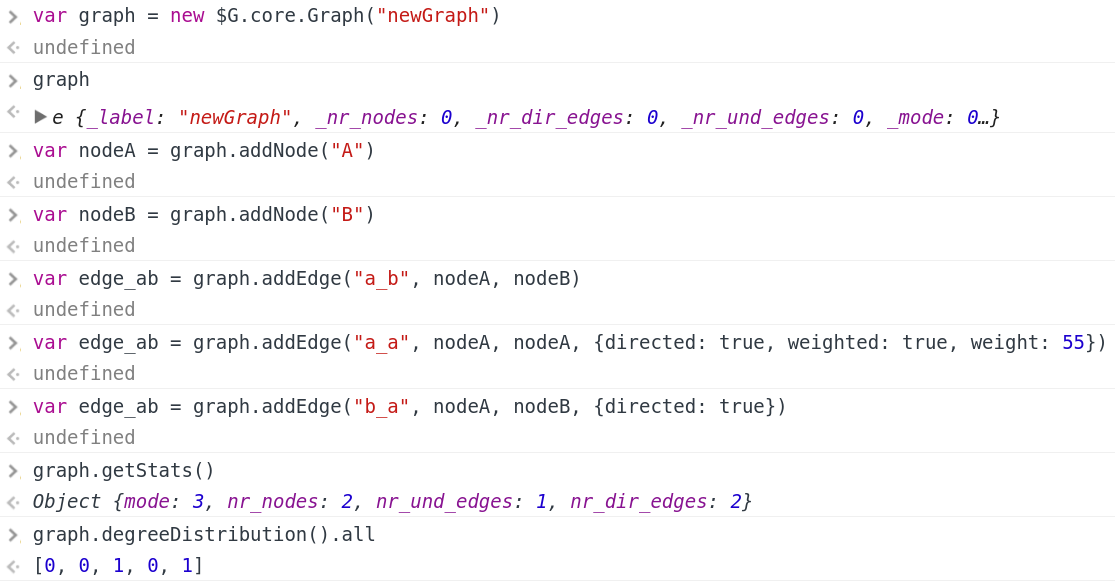
\includegraphics [width=1\textwidth] {figures/buildGraphManually}
			\caption{Manually building a new graph in the console.}
			\label{fig:build_graph_manually}
		\end{center}
	\end{figure}
	
	
	\subsection{Load predefined graph and visualize}
	\label{ssect:load_graph}
	
	Using either the CSV or JSON Reader build into GraphiniusJS, we can also request to instantiate a graph from a remote file. Here we use the JSON Reader to load a graph depicting a nevus and render it using GraphiniusVIS (Figure~\ref{fig:load_graph_repl}). Apart from the visualization, we also compute its degree distribution.
	
	\begin{figure}[H]
		\begin{center}
			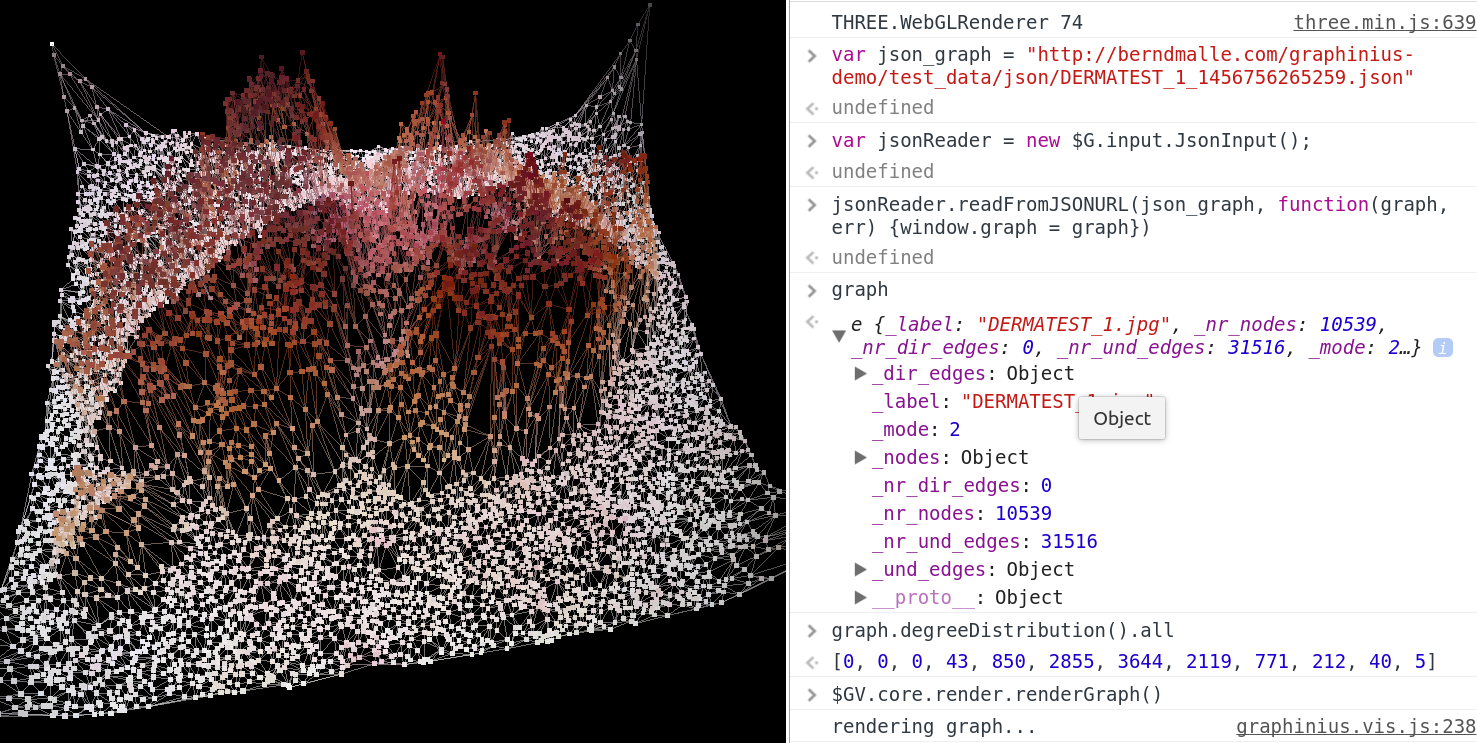
\includegraphics [width=1\textwidth] {figures/loadingGraphInREPL}
			\caption{Loading a JSON graph and visualizing it via the browser console.}
			\label{fig:load_graph_repl}
		\end{center}
	\end{figure}
	
	
	\subsection{Run a BFS algorithm and visualize}
	\label{ssect:run_bfs_visualize}
	
	After loading a (undirected) graph according to the previous section, we choose a random start node and invoke a breadth-first-search algorithm resulting in a \textit{distance map} centering around that node. The following lines of code (Figure~\ref{fig:color_graph_bfs}) show distances and parents of a selection of nodes (note the parent / distance chain...) while the accompanying visualization colors the graph according to the obtained distances via gradient computations (the start node being colored green and the node with maximum distance being colored red).
	
	\begin{figure}[H]
		\begin{center}
			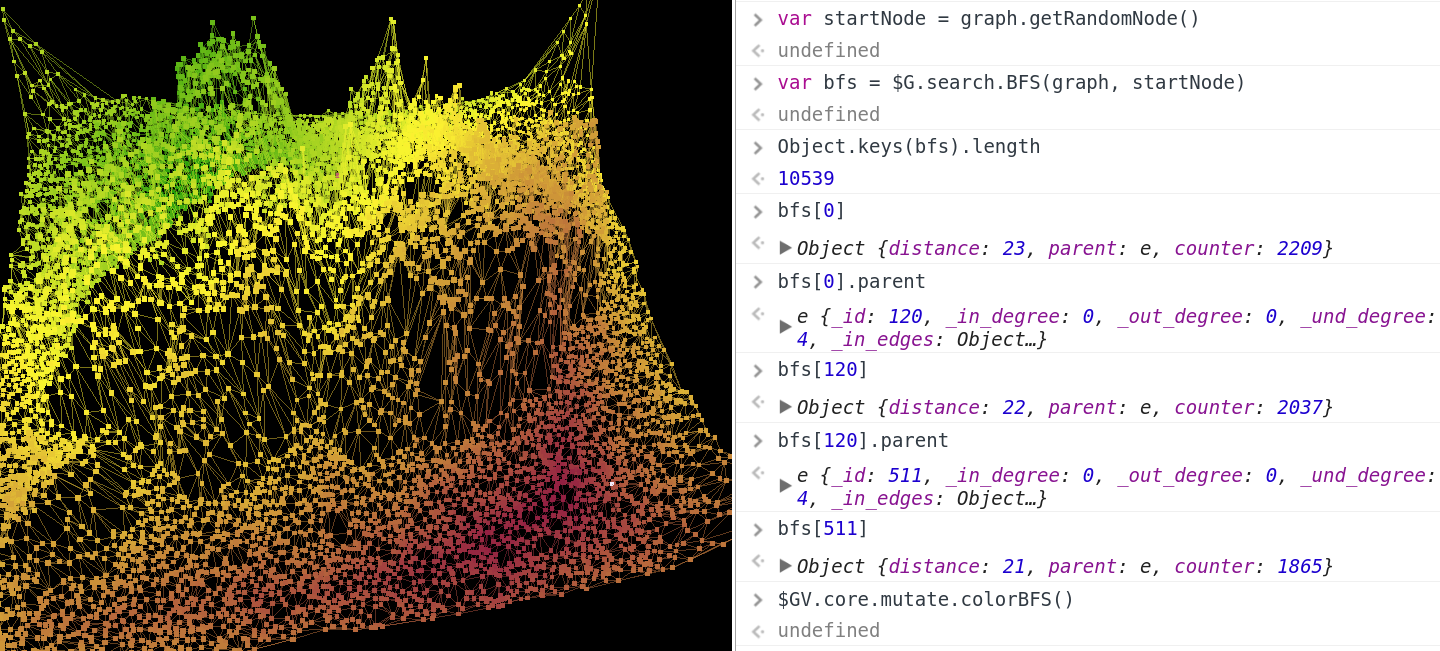
\includegraphics [width=1\textwidth] {figures/colorBFSREPL}
			\caption{Computing a BFS in a live browser REPL \& visualizing the result.}
			\label{fig:color_graph_bfs}
		\end{center}
	\end{figure}
	
	
	\subsection{Run a DFS algorithm and visualize}
	\label{ssect:run_dfs_visualize}
	
	Lastly, in Figure~\ref{fig:color_graph_dfs} we load the same graph as before, this time interpreted as a directed graph, choose a random start node again and invoke a DFS algorithm. This returns to us an array of graph segments representing the node sets reachable from each start node of a respective DFS Visit run (had we chosen an undirected graph, there would only be a single segment). We then output the size of each segment and again visualize the result, assigning to each segment a different color.
	
	\begin{figure}[H]
		\begin{center}
			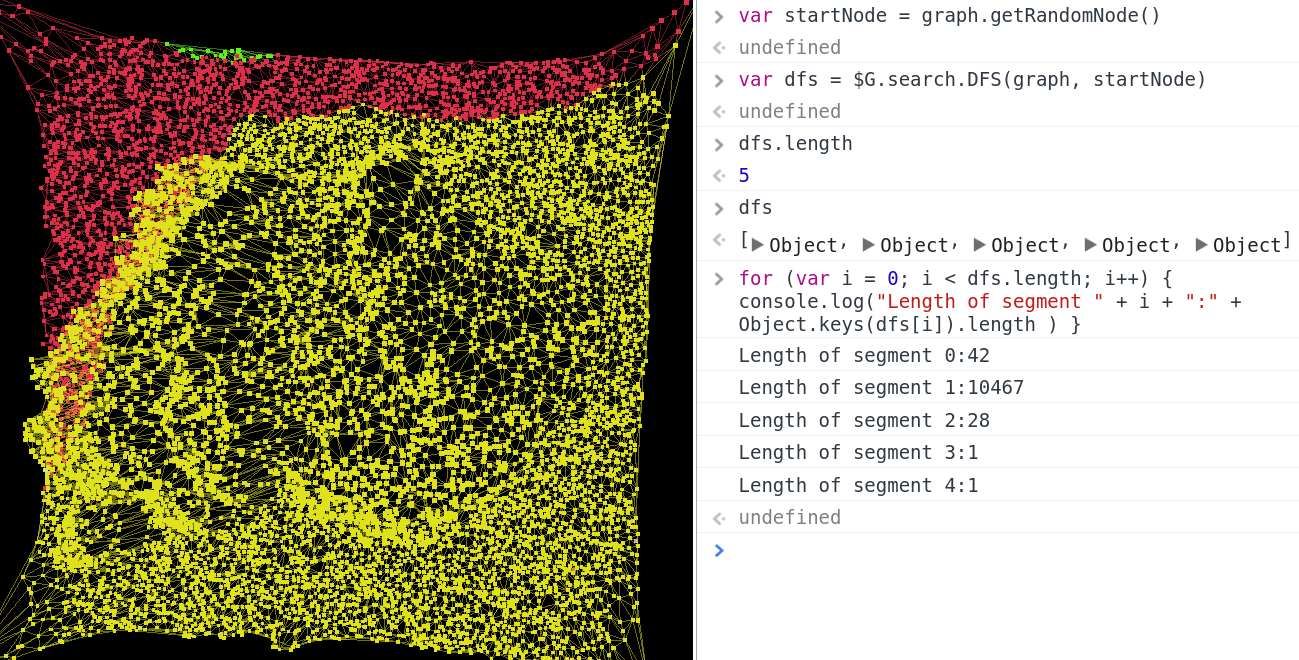
\includegraphics [width=1\textwidth] {figures/colorDFSREPL}
			\caption{Computing a DFS in a live browser REPL \& visualizing the result.}
			\label{fig:color_graph_dfs}
		\end{center}
	\end{figure}	


\section{Graph extraction from images}
\label{sect:graph_ext}
	
	In order to be able to apply graph theory to problems originating in the realm of image processing, first we need to extract a graph structure out of an image. There are potentially many different ways of doing this; as described in our paper \citep{GraphExtractPaper}, we are executing the following steps:
	
	\begin{enumerate}
		\item \textbf{Image preprocessing.} Many image segmentation algorithms use gray scale values to compute distances between neighboring pixels, gradients etc. (it seems that using 3 color channels per pixel is not much superior over using just one).
		\item \textbf{Input image as graph.} The resulting image is simply interpreted as a graph, which is possible because every pixel-based image naturally forms a graph structure, in which pixels are represented by nodes and neighborhoods are represented by edges. We then extract an edge list where the entries is sorted according to edge weight (= differences in the intensity values of neighboring nodes).
		\item \textbf{Graph based (over-)segmentation.} As the next step, a Kruskal MST based algorithm developed by \citep{FelzenszwalbHuttenlocher2004} is applied. It takes the approach of merging regions from pixel level (= inital nodes) 'upwards' instead of recursively partitioning the whole image 'downwards' - essentially, at every step it compares an intra-region coherence measure to an inter-region similarity measure:
		
			\begin{equation*}
			\text{Int}(C) = \max\limits_{e \in \text{MST}(C,E)}  \omega(e)
			\end{equation*}
			is the intra-region coherence value, given by the maximum edge weight of the region's MST.
			
			\par
			\begin{equation*}
			\text{Dif}(C1,C2) = \min\limits_{v_i \in C1, v_j \in C2, (v_i,v_j) \in E} \omega(v_i,v_j)
			\end{equation*}
			denotes the intra-region similarity measure, given by the minimum edge weight connecting any two nodes between them.
			
			\par Finally,
			\begin{equation*}
			\text{D}(C1,C2) = \left\{
			\begin{array}{l l}
			\textit{true} & \quad \text{if} \quad \text{Dif}(C1,C2) > \text{MInt}(C1,C2)\\
			\textit{false} & \quad \text{otherwise}
			\end{array} \right.
			\end{equation*}
			determines if two regions should be merged, based on the relation of their intra-region coherence and inter-region similarity measures.
			
			\par Once all edges have been considered, the final graph partition represents the segmentation (merging) result
		
		\item \textbf{A Delauney triangulation} is computed once the final region map has been established, taking each region's centroid to become a node in the new graph, as well as the (non-overlapping, as the algorithm is producing a tessellation of the region map) connections between those centroids to be their respective edges. The edge weight is computed from the difference in average intensity value of two adjacent regions.

		\item \textbf{Graph output.} Those data are finally transferred into a JSON structure consumable by Graphinius JS, as depicted by the sample JSON graph in Figure~\ref{fig:json_input_graph}.
	\end{enumerate}
	
	With the exception of manually written micro-graphs for the sake of rapid unit testing, this procedure was used for practically all JSON graphs  employed in the development and testing of GraphiniusVIS. Due to the flexibility of the algorithm - it features 3 separate parameters which control the granularity of the partition, and therefore the granularity of the graph structure - it was possible to extract graphs from a few hundred nodes and edges to up to 22k nodes / 66k edges. The average execution time on the author's quad-core i5 machine lay in the range of 3-5 seconds.
		
	\begin{figure}[H]
		\begin{center}
			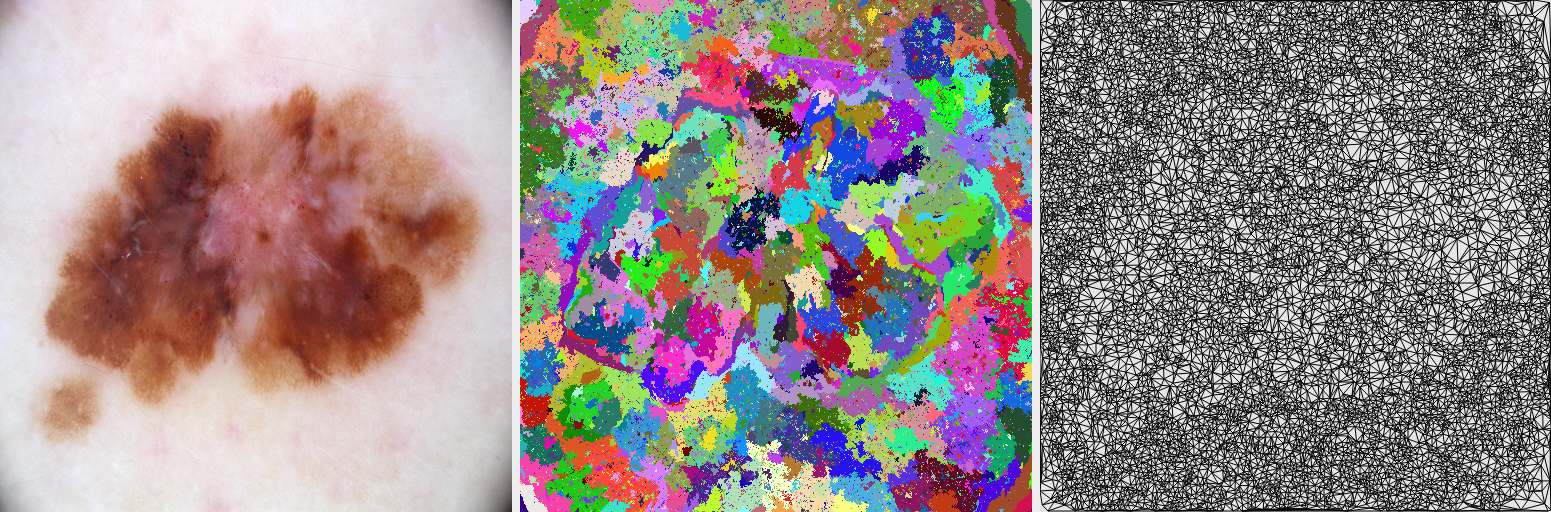
\includegraphics [width=1\textwidth] {figures/graph_ext}
			\caption{Kruskal MST based region merging \& graph extraction.}
			\label{fig:graph_extract}
		\end{center}
		\small 
		Result of applying a Kruskal based region merging algorithm to an image of numerous small scale regular structures. (1) Input image, (2) 
		
	\end{figure}


\section{Anonymity: SaNGreeA (with iML)}
\label{sect:aoa_anonymization}

	\begin{enumerate}
		\item \textbf{Process input data into suitable structure}
		\item \textbf{Enhance structure with graph information (random)}
		\item \textbf{Anonymize via SaNGreeA}
		\item \textbf{prepare individual cost function via iML}
		\item \textbf{Anonymize via SaNGreeA modified}
		\item \textbf{Compare results}
	\end{enumerate}
	
	\begin{figure}[ht]
		\begin{center}
			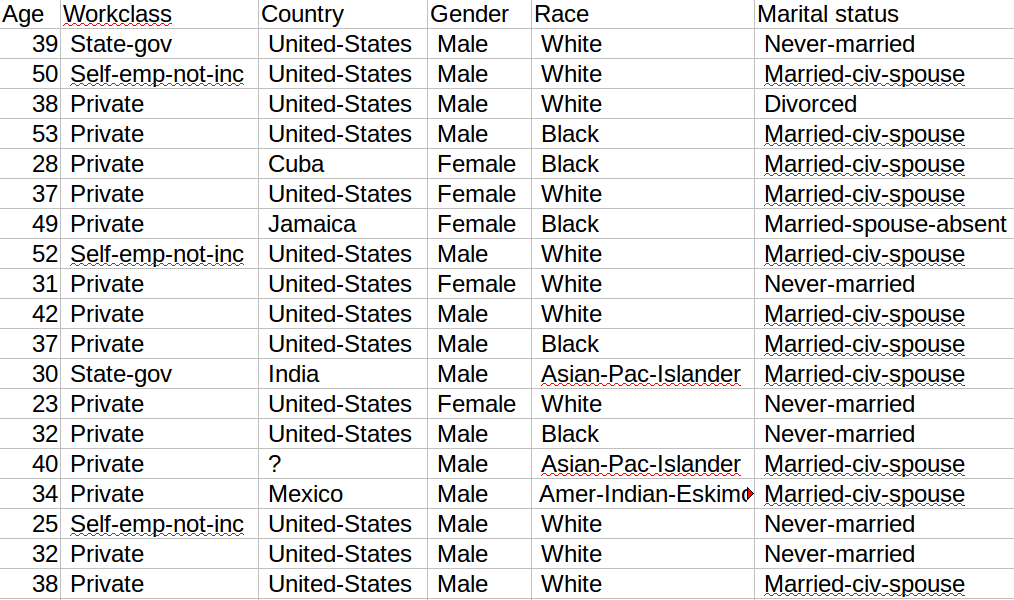
\includegraphics[width=1\textwidth]{figures/anonym/anon_adults_input_sample_pic}
			\caption{Excerpt: the first 25 rows of the Adult census data set}
			\label{fig:anonIML}
		\end{center}
	\end{figure}





\chapter{Results and Discussion}
\label{ch:results_discussion}


\section{Size of codebase}
\label{sect:complexity}


\section{Test coverage}
\label{sect:test_coverage}

Testing is a great practice to guide the development and programming effort while conducting a software project, but it is of equal importance as a documentation tool allowing the technical staff to demonstrate to their clients (customers and managers alike) the care they exercised in constructing their codebase. Coverage testing detects if parts of the codebase were either just partly tested or not tested at all, taking into account LOC coverage, percentage of functions / methods invoked as well as branch or general statement coverage.

As can be seen in Figure~\ref{fig:test_coverage}, Graphinius JS has been exhaustively tested, reaching 100\% coverage for all but the branches department. The lower value in this section is a result of \textit{else-branches} not taken, in cases when there was no \textit{else-branch} to take. This can be remedied by re-writing all \textit{if-statements} in the form of \textit{(boolean condition \&\& consequent)}, so that the code coverage tool does not recognize the \textit{if} keyword. The author has successfully tested this practice on the PFS.ts file (as can be seen in Figure~\ref{fig:test_coverage}) but at the time of this writing considers it inappropriate to alter perfectly good code throughout the library just for the sake of artificially achieving 100\% coverage.

\begin{figure}[ht]
	% \centering
	\hspace*{-0.5cm}
	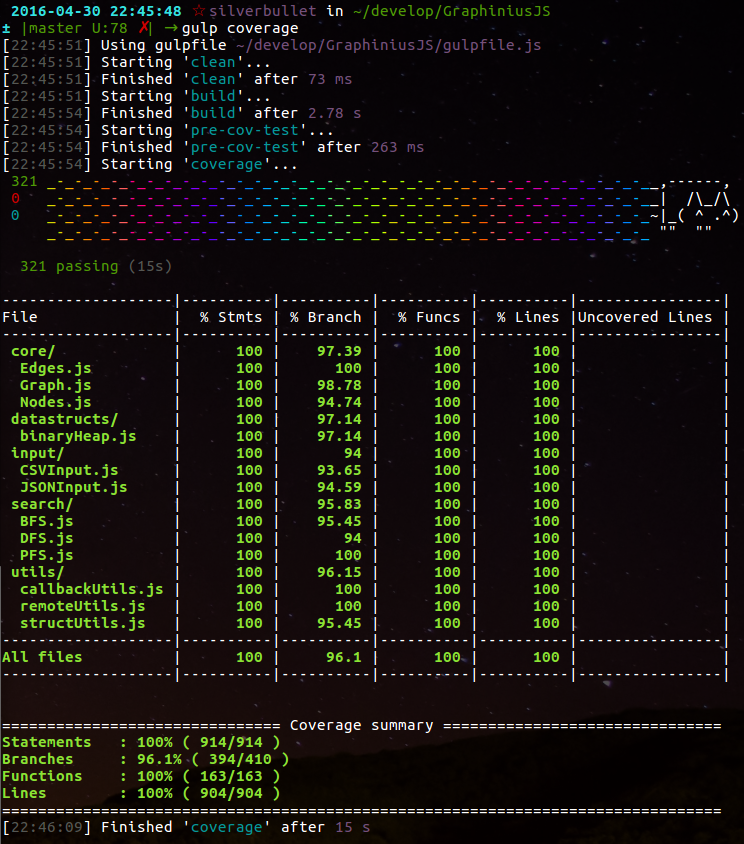
\includegraphics[width=1.1\textwidth]{figures/test_coverage}
	\caption{GraphiniusJS test coverage}
	\label{fig:test_coverage}
\end{figure}


\section{Performance compared to selected libraries}
\label{sect:perf_other_libs}

	\subsection{iGraph (c++)}
	\label{ssect:perf_igraph}
	
	\subsection{Graph Tool}
	\label{ssect:perf_graphtool}
	
	\subsection{NetworkX (pure python)}
	\label{ssect:perf_networkx}
	
	\subsection{Graphinius JS}
	\label{ssect:perf_graphinius}
	

\section{Execution speed in various scenarios}
\label{sect:performance}

	\subsection{graph loading}
	\label{ssect:perf_graph_loading}
	
	\subsection{degree distribution}
	\label{ssect:perf_deg_dist}
	
	\subsection{BFS / DFS}
	\label{ssect:perf_bfs_dfs}
	
	The test was performed on a graph of 


\section{Discussion of results}
\label{sect:discussion}
	

\chapter{Open Problems \& Future Work}
\label{ch:future_work}



\section{Future Work}
\label{sect:future_challenges}

Considering GRAPHINIUS an arbitrarily extendable computing platform (which uses graphs as underlying, universal data structures), there are many possibilities to build upon this work, ranging from small improvements to the introduction of fundamentally new infrastructure, transcending the use of contemporary graph libraries. 

The use of a centralized, Web based graphical workflow system will prove especially useful in exploiting and propagates the experience of individual users, as it bundles not only data, but also the settings and results of all experiments conducted on that platform.


\subsection{Graph generators (graph types)}
\label{ssect:graph_gen}


\subsection{Graph classifiers}
\label{ssect:graph_class}


\subsection{JSVM based grid computing}
\label{ssect:jsvm_grid}


\subsection{General processing / ML pipelines}
\label{ssect:pipelines}

As existing stacks indicate, there are several possible levels of pipelines which can be sorted by increasing homogeneity amongst their stages as well as decreasing technical demands on their users:

\begin{itemize}
	\item Level 0: Writing all of the pipeline manually. As every combination of technologies are usable, this approach gives the most flexibility but is hard to maintain and almost impossible to reproduce. As \citep{MLTechnicalDebt} perfectly states: ``Using self-contained solutions often results in a glue code system design pattern, in which a massive amount of supporting code is written to get data into and out of general-purpose packages.''
	
	\item Level 1: Automated, but self designed and coded. This entails the usage of tools like Unix Make, which is language agnostic and therefore supports any number of technologies as long as they are executable from a Shell. Apart from slightly better decoupling, same problems as Level 0.
	
	\item Level 2: Establishing a common understanding of the components and structure of a pipeline while still using individual technologies. Such a common standard exists in the form of PMML - the Predictive Model Markup Language. PMML defines stages of pipelines as well as their inputs, parameter types and ranges, the output format etc. Thus, developers can use their favorite technologies in the development phase while PMML consuming tools then produce familiar code (Hadoop, Spark, ..).
	
	\item Level 3: Language specific libraries exposing an API to conveniently assemble a pipeline. Such libraries have been released by projects like scikit-learn or Apache Spark. While currently becoming popular, APIs still restrict the creation of data applications to experts capable of coding.
	
	\item Level 4: The use of a custom DSL would widen the ability to create complex data pipelines to any kind of domain expert. Similar in nature to SQL, it is able to either compile itself into code or an intermediate representation like PMML.
	
	\item Level 5: A fully integrated data analysis platform that offers intuitive, visual pipeline assembly. Ideally, tools for reporting, reproduction and collaboration would also be included. In addition, the platform could offer experts the means to write stages themselves via an online code editor. OGMA is designed to be such a platform.
\end{itemize}


\subsection{Heterogeneous data linkage}
\label{ssect:heterogeneous_data}

Many research fields comprise several sub-problems which are amenable to different machine learning approaches and feature their own, distinctive input data sets. Coming from various, different data sets featuring their distinct attribute domains, they probably are - via their time-, space- or other dimensions, interlinkable with one another. Usually, studies are only concerned about using a single one of those data sources and applying different methods to it. However, a more holistic approach would be to fuse those data sets along one or more dimensions (or any other meaningful ruleset) in order to achieve a richer representation of the underlying problem. A resulting data-set might take the form of a graph structure, in which individual entities from the originating sets are linked by meaningful connection rules, which in themselves will have to be learned. 

%For example, \cite{thebook} introduced the concept of authority ranking for heterogeneous networks, where the impact is transferred along edges to simultaneously rank nodes of different types.

\subsection{Meta machine learning}
\label{ssect:meta_ml}

Meta-learning applies learning algorithms on data collected about machine learning experiments. As one of the first papers regarding this topic, \citep{Rice1975} defined the "Algorithm Selection Problem", which was first recognized as a meta learning problem by the machine learning community. He describes five spaces in which the Algorithm Selection Problem plays out:

\begin{itemize}
	\item \textbf{The problem space}: This is the set of all possible input problems (datasets + desired result class).
	
	\item \textbf{The feature space}: Features of a specific problem or family of problems. In dermatological imaging those would be defined by the imaging method (laser-scan vs. stanza), the scale of the objects to be detected (single cells vs nevi) etc.
	
	\item \textbf{The algorithm space}: The set of all algorithms suitable for the specific problem (features) to be worked on.
	
	\item \textbf{The performance measures} (the metric space): The set of possible measurements that could describe the quality of a solution (runtime performance, accuracy, ..).
	
	\item \textbf{The criteria space}: The weighing of different performance measures considered for a particular solution.
\end{itemize}


In most scenarios concerning Graphinius we will be concerned with the selection of workflow components and their parameters based on the nature of the specific area of application, the tackled problems, their features, available algorithms, preprocessing methods, parameters as well as performance measures.

\subsection{Hyper heuristics}
\label{ssect:hyper_heuristics}

Hyper heuristics are a way of selecting or configuring algorithms by searching a space of lower level heuristics instead of searching the solution (parameter) space itself. Hyper heuristics are different from meta learning in that they work independently of the problem domain and therefore promise to be generally applicable; the challenges lie in producing algorithms that do not need to be optimal, but rather good-enough, soon-enough, cheap-enough \citep{Burke:2003:Hyperheuristics}.

Although many research fields in themselves are not broad enough to be a suitable proving ground for hyper heuristic research, the Graphinius platform will provide us with meta-data about experiments in many diverse areas. We fully agree with \cite{Burke2013} who concludes that there is still little interaction between research communities, a problem whose solution could lead to the extension of algorithms to both new problem domains and new methodologies through cross-fertilization of ideas.


\subsection{Meta ML / heuristics database}
\label{ssect:heuristics}

The greatest advantage of using Meta ML in combination with a centralized, Web based workflow system lies in the fact that users may profit from their colleagues' meta data by building up a collective Meta ML database: input data plus algorithm parameters plus success metrics.


\subsection{Algorithmic recommender}
\label{ssect:algo_recommender}


\chapter{Conclusion}
\label{ch:conclusion}

In this thesis we have introduced the Graphinius platform for graph-theoretical Machine Learning experiments built on Web technologies, employing in-browser computations as well as visualization, focusing on a community centered approach.

After discussing some theoretical advantages such a platform could offer in the first chapter and delving into more specific descriptions of the theoretical underpinnings of potential application areas, we also took an interest in how such a product could be marketed, what business models would support it, and where the main advantages lie over its foreseeable competitors.

A generic description of the platform characteristics was given, followed by an in-depth survey of the modern web development cycle, its components and supporting infrastructure. Sifting through a wealth of open source alternatives, we finally decided on how to build every component of the Graphinius ecosystem including the base library, visualization, and communication (history) module.

We saw how three different use cases, theoretically tackled in earlier chapters, can be implemented using Graphinius and presented the output of their respective computations.

Following the presentation of some implementation metrics, such as size of the codebase and performance measurements on different graphs, we finally conducted a rather extensive sweep of interesting challenges and the promise emerging technologies hold for future developments of the platform.

The Graphinius development is still in its early phases, with just a groundwork having been laid as of May, 2016. Remembering the first conception of Graphinius only about six months earlier however, the author is remarkably pleased with the progress and dares to take a very optimistic look into the future.



\appendix
% \noappendicestocpagenum
% \addappheadtotoc
%\chapter{Data Schema}
%\label{App:AppendixA}

% \lstinputlisting[language=json]{listings/models.js}

\chapter{Anonymization Tables}
\label{App:AppendixA}

\section{Input data}
\label{sect:anon_input_data}

\section{Anonymized data}
\label{sect:anon_output_data}

{
\setstretch{1}
%\csvreader[
%longtable=llllll,
%table head=
%\toprule\bfseries Age range & \bfseries Employment & \bfseries Country & \bfseries Gender & \bfseries Race & \bfseries Marital status \\ \midrule\endhead
%\bottomrule\endfoot,
%late after line=\\,
%before reading={\catcode`\#=12},after reading={\catcode`\#=6}
%]{figures/anonym/adults_300_anon_k10.csv}{1=\age,2=\employed,3=\country,4=\gender,5=\race,6=\marital}{\age & \employed & \country & \gender & \race & \marital}
}

\chapter{GraphiniusJS API}
\label{App:AppendixB}

\begin{landscape}
	%\includepdf[pages={1-84}, 
	%nup=1x2,
	%landscape=true,
	%width=.90\textwidth,
	%trim=0 0 30pt 0,
	%keepaspectratio
	%]{figures/graphinius_doc.pdf}	
\end{landscape}
      % Appendix A


\cleardoublepage
\phantomsection
\addcontentsline{toc}{chapter}{List of Figures}
\listoffigures

\cleardoublepage
\phantomsection
\addcontentsline{toc}{chapter}{List of Listings}
\lstlistoflistings

%\cleardoublepage
%\phantomsection
%\addcontentsline{toc}{chapter}{List of Tables}
%\listoftables

% \cleardoublepage
% \phantomsection
% \addcontentsline{toc}{chapter}{Glossary}
% \printglossary

% \cleardoublepage
% %!TEX root = thesis.tex


      % Abbreviations

\cleardoublepage
\phantomsection
\addcontentsline{toc}{chapter}{References}
%!TEX root = thesis.tex

% harvard styles: http://tex.loria.fr/bibdex/harvard.pdf
%\bibliographystyle{dinat}
%\bibliographystyle{agsm}
%\bibliographystyle{unsrtnat} % plainnat, abbrvnat
%\bibliographystyle{plainnat}
%\bibliographystyle{apalike}

\addcontentsline{toc}{chapter}{References}

%\bibliography{thesis-references}

\printbibliography






\end{document}

